\documentclass[a4paper]{book}

\usepackage[parts]{classicthesis}
\usepackage[eastereggs,extras]{cmcq}
% \usepackage[eastereggs,extras,print]{cmcq}

\title{\textsf{Computational Models and Complexity Questions}}
\author{Alessandro Clerici Lorenzini}
\date{Academic Year 2023/2024}

\begin{document}

\frontmatter

\maketitle

% \extra{\openingquote{"It's a mistake to try and understand mathematics.\\They only worry me."}{From \textit{Life, the Universe and Everything}\nocite{Ada82}}}
\extra{\openingquote{"It's a mistake to try and understand machines.\\You end up worrying too much."}{From \textit{Life, the Universe and Everything}\nocite{Ada82}}}

\extra{\chapter*{Acknowledgements}
In the course of my Master's degree, I experienced a number of adventures.
I met peers of great intelligence, inspiring professors, and exceptionally talented researchers.
I lived and studied in three different countries, finding new value in what I had and discovering it in what I didn't know.
% I had some of the best and some of the worst times of my life.
I experienced some of the best and some of the most challenging moments of my life.
% But you take what you can get, and you make the most of it.
But when you're down you're down, and when you're up you're up.
And while I am slowly finding my way into this weird, wonderful world, there's still a million things I haven't done.
It is in moments like this, at the end of a journey that had such a profound impact on life, that one has to take a moment to reflect on what made it possible, and what made each day a little bit better.

I would like to thank Giovanni Pighizzini and Luca Prigioniero, whose competence as supervisors matches their excellence as researchers.
In particular, I would like to express my deepest gratitude to Luca Prigioniero.
Not only did he carry out his role as co-supervisor with the utmost expertise and helpfulness, but I found in him a mentor and, ultimately, a friend.
% A heartfelt thanks goes to my parents, who never ceased to support me, and without whom none of this would be possible.
A heartfelt thanks goes to my family: my parents, whose constant support made all of this possible, and my sister Francesca, with whom I have enjoyed many memorable sibling moments, and in whom I have found an unexpected friend.
I am also deeply grateful to my peers and friends from Milan, Copenhagen, and Loughborough, who were the very heart of this journey and kept me going day after day.

Finally, my heartfelt thanks go to the professors and researchers whose passion for their work inspires and motivates others.
They are the true heart of the university.

\vskip 5mm

\noindent But look at me still talking when there's science to do\dots

\vskip 5mm

\hfill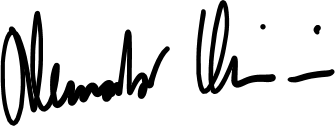
\includegraphics[scale=1.3]{img/signature.png}\hspace{3mm}\raisebox{3.5ex}{\tikz\Aleduck[scale=.35];}
}

\tableofcontents

\addcontentsline{toc}{chapter}{List of Figures}
\listoffigures
\addcontentsline{toc}{chapter}{List of Tables}
\listoftables

\mainmatter

\setcounter{chapter}{-1}
\chapter{Introduction}
After millennia of human history, in which we repeated the same actions over and over, people started wondering if those actions could be done automatically.
Computer Science was born with the prospect of answering two questions: "what problems can be solved automatically?", and "how many resources would it cost?".

Theoretical computer science developed throughout the years several ways of describing automation, one of them being computational models.
Such concepts are studied in Formal Language Theory, and consist in mathematical objects (machines) that process strings of characters.
Each of these machines can recognize what strings belong to a certain set, called the accepted language.
Different types of machines can accept different classes of languages, bringing to the questions of their equivalence and their comparison in size.
Descriptional Complexity studies ways of describing languages, including computational models, in terms of how succinct they can be.

The innermost class of the classic hierarchy of languages (the Chomsky hierarchy~\cite{Cho56}) is the one of regular languages, famously recognized by finite state automata.
An important open problem of Descriptional Complexity is the Sakoda and Sipser conjecture~\cite{SakSip78}, regarding the size trade-off between nondeterministic and deterministic regular language acceptors.
The most powerful computational model is the Turing Machine, composed by a tape with an infinite number of cells, a head which scans and possibly writes on one cell at a time, and a finite state memory.
Many restrictions of the Turing Machine have been studied, by comparing their accepting power with the ones of other models.

Limited automata were introduced by~\citeauthor{Hib67} in~\citeyear{Hib67} as a restriction of nondeterministic Turing Machines~\cite{Hib67}.
% Given an integer~$k$, a $k$-limited automaton has a finite tape, initially containing the input string and delimited by special symbols called end-markers, and can only write on each tape cell on its first~$k$ visits.
Given an integer~$k$, a $k$-limited automaton has a finite tape, initially containing the input string, and can only write on each tape cell on its first~$k$ visits.
In~\citeyear{WagWec86},~\citeauthor{WagWec86} proved that when~$k=1$ such machines accept regular languages~\cite{WagWec86}.
Later,~\citeauthor{PigPis14} proved that their simulation by deterministic finite state automata can require a double exponential growth in size, making $1$-limited automata much more succinct~\cite{PigPis14}.

The discovery of a new succinct model for regular languages sparked a new interest for limited automata, leading to the study of several variations of the model, with the hope of a new perspective on tackling the Sakoda and Sipser problem.
In this work, we studied two models in particular: \emph{sweeping} $k$-limited automata, and \emph{once-marking} $1$-limited automata.



\section{Structure of the thesis}
The work is divided into chapters:
\begin{description}
	\item[\Cref{ch:context}] We give an overview of the motivation behind our work and the history of the literature around the studied problems.
	\item[\Cref{ch:preliminaries}] We formally describe the main concepts of automata theory and descriptional complexity that are relevant to our work.
	\item[\Cref{ch:techniques}] We show a few techniques used in the simulation of two-way finite automata by one-way finite automata.
	\item[\Cref{ch:sweeping}] We present a construction for the simulation of deterministic sweeping $k$-limited automata by nondeterministic finite state automata, based on the techniques showed in the previous chapter. We discuss descriptional complexity aspects, showing that the simulation has an exponential cost in size, and present a matching weak lower bound.
	\item[\Cref{ch:nondetsweep}] We explain how the simulation in the previous chapter can be extended to the nondeterministic case.
	\item[\Cref{ch:oncemarking}] We summarize our investigations about the model of once-marking limited automata, in our attempts to improve upper and lower bounds for their simulation by other equivalent recognizers.
	\item[\Cref{app:results}] We summarize descriptional complexity results around the simulations between regular language acceptors, including $1$-limited automata and once-marking limited automata.
	\item[\Cref{app:constructions}] We show few constructions on finite state automata that let us make simplifications across the main chapters.
\end{description}

\chapter{Context and motivation}



\section{Formal languages and automata theory}
Formal language theory is a fundamental field of theoretical computer science that studies \emph{languages}, \ie sets of strings, and finite ways to represent them.

\paragraph{Language descriptions} The finite representations of languages span different paradigms: for example, we might state a property that holds on the strings belonging to the language, or construct a generative or a recognizing model.
Generative models, typically \emph{grammars}, define a list of rules that can be used to generate the strings in the desired language.
Recognizing \emph{computational models} consist in abstract machines that can determine, in a certain number of steps, if a given string belongs to the chosen language.

\paragraph{The Chomsky hierarchy} Different models for the description of languages characterize possibly different language classes, originating what is commonly known as the \emph{Chomsky hierarchy} \cite{Cho56}.
\ironic{Although his attempt to create a model generating the English language failed miserably, \citeauthor{Cho56} accidentally founded an entire field of computer science, which is somehow still researched to this day by people like the undersigned.}{}
The hierarchy, originally described for grammars, spans four language classes, each strictly containing the following:
\begin{itemize}
	\item \emph{recursively enumerable}, characterized by Turing machines,
	\item \emph{context-sensitive}, characterized by linear bounded automata,
	\item \emph{context-free}, characterized by pushdown automata,
	\item \emph{regular}, characterized by finite state automata.
\end{itemize}

\paragraph{Nondeterminism} A very important concept in formal language theory is the one of \emph{nondeterminism}.
At a given time of its computation, a nondeterministic machine has possibly multiple choices on the next step, which implies the possibility of several computation paths given the same input.
We say that a nondeterministic machine accepts a string if there exists a computation path over that string which brings the machine to accept.

One of the very first problems in the field was to determine if the nondeterministic and deterministic variants of the same computational model accepted the same language class.
While this was found to be the case for the canonical recognizers of recursively enumerable, context-sensitive and regular languages, \citeauthor{Fis63} and \citeauthor{Sch63} proved that deterministic pushdown automata accept a smaller class than their nondeterministic counterpart, called \emph{deterministic context-free languages} \cite{Fis63,Sch63}.
Concerning the regular language class, \citeauthor{RabSco59} found in \citeyear{RabSco59} a construction, known as the \emph{subset} (or \emph{powerset}) \emph{construction}, to convert a nondeterministic finite automaton into a deterministic one \cite{RabSco59}.

\paragraph{Two-way models} In the same article, \citeauthor{RabSco59} defined \emph{two-way} nondeterministic and deterministic \emph{finite automata} (\TNFA and \TDFA, respectively).
These models act in a similar way to the classic, one-way finite automata (\ONFA and \ODFA), where the input is read one symbol at a time and the machine changes state depending on the scanned symbol and the current state. However, while one-way machines read the input symbols subsequently from left to right, two-way models can move left or right freely, as described by the transition rules.
\citeauthor{RabSco59} proved that these new models also characterize regular languages, by simulating them with a \ONFA with a construction based on \emph{crossing sequences} (more in \Cref{sec:crossseq2DFA}) \cite{RabSco59}.
The same result was found in parallel by \citeauthor{She59}, who used a different construction based on \emph{transition tables} and that also works with a deterministic simulating machine (see \Cref{sec:transtab2DFA}) \cite{She59}.



\section{Descriptional complexity}\label{sec:context-descrcomp}

\paragraph{Model size bounds} With many equivalent computational models accepting the same language classes, questions naturally arose about comparing them to one another.
In \citeyear{MeyFis71}, \citeauthor{MeyFis71} proposed to compare different descriptions for a language class by their size, that is, by how succinctly they can describe the chosen language \cite{MeyFis71}.
Concretely, this typically means comparing the size of the components of the models, such as the number of states or the size of the working alphabet.

From the construction given by \citeauthor{RabSco59}, it followed that each nondeterministic finite automaton can be simulated by a deterministic one by paying an exponential cost in the number of states.
In their article, \citeauthor{MeyFis71} proved that there exist families of languages for which this difference in size cannot be reduced, therefore giving a tight bound on the cost of removing nondeterminism from one-way finite automata \cite{MeyFis71}.
\citeauthor{Moo71} achieved the same result independently in the same year \cite{Moo71}.

See \cite{KutMor+21} for a recent overview of descriptional complexity results and problems of interest.

\paragraph{The Sakoda and Sipser conjecture} Given the exponential gap between the sizes of the nondeterministic and deterministic one-way models, the natural next step was to compare their two-way counterparts.
The afore-mentioned constructions by crossing sequences \cite{RabSco59} and transition tables \cite{She59} gave an exponential upper bound on the simulation of \TNFA or \TDFA by \ONFA or \ODFA.
An exponential lower bound on the simulation of \TNFA by \ODFA is a direct consequence of the one on the simulation of \ONFA by \ODFA.
Later, thanks to \citeauthor{Bir93} (\citeyear{Bir93}) and \citeauthor{Kap05} (\citeyear{Kap05}), matching exponential lower bounds were found for the simulations of \TDFA by \ONFA and \ODFA and of \TNFA by \ONFA \cite{Bir93,Kap05}.
These descriptional complexity results for regular language acceptors, summarized in \Cref{tab:sims-core-general-context}, leave two open problems (highlighted in red): the simulations by \TDFA of \TNFA and \ONFA.

\begin{table}
	\centering
	\renewcommand{\hstdef}{.35}
\begin{tabular}{|l|l|l|p{2.9em}|l|}
	\hline
	~     & \ODFA   & \ONFA     & \TDFA                          & \TNFA     \\ \hline
	\ODFA & \cY     & $\Cctriv$ & $\Cctriv$                      & $\Cctriv$ \\ \hline
	\ONFA & $\Cexp$ & \cY       & \cR $\le\Cexp\hst$ $\ge\Cpoly$ & $\Cctriv$ \\ \hline
	\TDFA & $\Cexp$ & $\Cexp$   & \cY                            & $\Cctriv$ \\ \hline
	\TNFA & $\Cexp$ & $\Cexp$   & \cR $\le\Cexp\hst$ $\ge\Cpoly$ & \cY       \\ \hline
\end{tabular}
%
	\caption[Costs of the simulations between regular language recognisers.]{Costs of the simulations between regular language recognisers.
		The red cells indicate the open problems featured in the Sakoda and Sipser conjecture.}
	\label{tab:sims-core-general-context}
\end{table}

These simulation costs were first discussed by \citeauthor{SakSip78} in \citeyear{SakSip78}, as the problem of using deterministic two-way movement to simulate nondeterministic computations \cite{SakSip78}, or, in other words, the elimination of nondeterminism from finite automata using the capability of scanning the input tape in a two-way fashion.
In their article, they described a parallelism between this problem and the famous \cP versus \cNP problem for time complexity classes, and conjectured that the costs of these simulations are exponential.

Later, new results around the unknown bounds were found, which gave them more importance in the realm of computational complexity.
Specifically, a relationship was found with the conjectured separation of the space complexity classes \cL and \cNL.
The class \cL is the set of languages accepted by deterministic Turing machines that write on a number of cells that is logarithmic in the length of the input, while \cNL is the set of languages accepted by nondeterministic such Turing machines.
The two classes are believed not to be equal, but no proof has been found yet, making this problem the analogous for space complexity of the famous problem of \cP versus \cNP.
\begin{enumerate}[(i)]
	\item\label{itm:LvNL-1} In \citeyear{BerLin77}, \citeauthor{BerLin77} proved that if $\cL=\cNL$, then every $n$-state \TNFA can be converted into a \TDFA of polynomial size in $n$ that accepts a string $w$ if and only if the original machine accepts $w$, for all strings $w$ of length at most $n$.
	      That is, if $\cL=\cNL$ then there exists a polynomial simulation of \TNFAs by \TDFAs on "short" inputs \cite{BerLin77}.
	\item In \citeyear{GefPig11}, \citeauthor{GefPig11} proved that in the \emph{unary case} the hypothesis on the input length posed by \citeauthor{BerLin77} is not needed.
	      Note that this implies that if a superpolynomial simulation of \TNFAs by \TDFAs is needed, even for the unary case, then $\cL\ne\cNL$ \cite{GefPig11}.
	\item In \citeyear{Kap14}, \citeauthor{Kap14} generalized \ref{itm:LvNL-1} for the class \cPolyL, the class of languages accepted by deterministic Turing machines that write on a number of cells that is logarithmic in the length of the input and can access a \emph{polynomial advice} \cite{Kap14,KarLip82}. In this case, the converse also holds.
	\item In \citeyear{KapPig12}, \citeauthor{KapPig12} proved that $\cNL\subseteq\cPolyL$ is equivalent to the existence of a polynomial size simulation of \TNFAs by \TDFAs for the unary case \cite{KapPig12}.
\end{enumerate}

Because of the importance of its potential repercussions, the Sakoda and Sipser problem has been tackled in many ways over the past decades, spanning four lines of development:
\begin{itemize}
	\item restrictions of the simulating machines (e.g. sweeping \cite{Sip80}, oblivious \cite{HroSch03}, and few reversals \cite{Kap13} automata),
	\item restrictions of the language classes (especially the unary case \cite{GefMer+07}),
	\item restrictions of the simulated machines (e.g. outer-nondeterministic automata \cite{GefGui+14,KapPig12}), and
	\item extensions of simulating machines (e.g. limited automata \cite{PigPis14,PigPri19,GuiPri19,PigPri+22}, linear-time Turing machines \cite{Pru14,GuiPig+18,Hen65,GuiPig+23,Har68}).
\end{itemize}
While the question remains open in the general case, these recent findings encourage new investigations on the topic.

An interesting review of old and recent results regarding two way automata and the Sakoda and Sipser problem, including a more in-depth analysis of some of the ones we mentioned here, was realized by \triplecite{Pig13}.


\section{Limited automata}
Limited automata were introduced by \citefullauthor{Hib67} in \citeyear{Hib67} with the aim of generalizing the notion of determinism in context-free languages \cite{Hib67}.
These devices are nondeterministic Turing machines with rewriting restrictions.
In particular, given a non-negative integer $k$, a \emph{$k$-limited automaton} (\kLA) is a machine with a single tape delimited to the cells initially containing the input by special symbols called end-markers ($\lem$,$\rem$), which can only write on each cell on its first $k$ visits.

In his seminal paper, \citeauthor{Hib67} proved that, for $k\ge2$, the class accepted by deterministic $k$-limited automata (\kDLA) is a strict subset of the class accepted by deterministic $(k+1)$-limited automata, hence generating an infinite, fine-grained hierarchy of context-free languages.
Only in \citeyear{PigPis15} it was proven that \DLA2 accept exactly deterministic context-free languages \cite{PigPis15}.
Furthermore, he proved that, for every $k\ge2$, nondeterministic $k$-limited automata characterize the class of context-free languages.
The latter result was proven by constructing simulations of \LA2 by models equivalent to pushdown automata and vice versa, along with reductions from $\kLA$ to $\LA{(k-1)}$.\footnote{%
	A simpler proof can be obtained as a consequence of the \emph{Chomsky-Shützenberger theorem} \cite{ChoSch63}, which states that every context-free language can be expressed as the homomorphic image of a \emph{Dyck language} (a language of balanced parentheses).
	A $\LA2$ accepting a Dyck language can be combined with a transformer applying the homomorphism, in order to accept any given language (see \cite{Pig19} for details).}

For $k=0$, the model coincides with two-way finite automata, therefore the accepting power is limited to regular languages.
In \citeyear{WagWec86}, \citeauthor{WagWec86} proved that the accepting power of a \TNFA does not improve if the machine can overwrite the content of each tape cell only on its first visit, namely $1$-limited automata characterize regular languages \cite{WagWec86}.

\paragraph{$1$-limited automata and descriptional complexity}
In \citeyear{PigPis14}, \citeauthor{PigPis14} resumed the study of limited automata with a new focus on descriptional complexity, as a new way to tackle the Sakoda and Sipser problem \cite{PigPis14}.
The size of a limited automaton can be expressed as a polynomial in the cardinalities of the state set and of the working alphabet.
By revisiting the proof given by \citeauthor{WagWec86}, \citeauthor{PigPis14} proved that an $n$-state \OLA can be simulated by a \ONFA with a number of states exponential in $n$.
Furthermore, they proved that if the \OLA is deterministic (\ODLA), the resulting finite automaton is also deterministic, while still exponential in size.
% Matching lower bounds were found thanks to a "block" language (a language defined by a proposition on same-sized factors of each word) witness that the simulations of a \OLA by a \ONFA or a \ODFA may need an exponential and double exponential size blow-up, respectively.
Matching lower bounds were found thanks to a language family witnessing that, in the worst case, the simulations of a \OLA by a \ONFA or a \ODFA need an exponential and double exponential size blow-up, respectively.
Thanks to the study of the unary case, \citeauthor{PigPri19} proved some of the remaining lower bounds, resulting in the costs summarized in \Cref{tab:sims-1la-general-context} \cite{PigPri19}.
The unary case was also studied by \citeauthor{KutWen15}, who proved state lower bounds for the simulation of unary \kLA by different variants of finite automata \cite{KutWen15}.

\begin{table}
	\centering
	\renewcommand{\hstdef}{.55}
\begin{tabular}{|l|l|l|p{3.1em}|l|l|p{3.1em}|}
	\hline
	~     & \ODFA              & \ONFA     & \TDFA                                            & \TNFA     & \OLA      & \ODLA                                            \\ \hline
	\ODFA & \cY                & $\Cctriv$ & $\Cctriv$                                        & $\Cctriv$ & $\Cctriv$ & $\Cctriv$                                        \\ \hline
	\ONFA & $\Cexp$            & \cY       & \cR $\le\Cexp\hst$ $\ge\Cpoly$                   & $\Cctriv$ & $\Cctriv$ & \cB $\le\Cexp\hst$ $\ge\Cpoly$                   \\ \hline
	\TDFA & $\Cexp$            & $\Cexp$   & \cY                                              & $\Cctriv$ & $\Cctriv$ & $\Cctriv$                                        \\ \hline
	\TNFA & $\Cexp$            & $\Cexp$   & \cR $\le\Cexp\hst$ $\ge\Cpoly$                   & \cY       & $\Cctriv$ & \cB $\le\Cexp\hst$ $\ge\Cpoly$                   \\ \hline
	\OLA  & \rbt[.2]{$\Cdexp$} & $\Cexp$   & \cG \rbt[.2]{$\le\Cdexp\hst[.1]$} $\ge\Cexp\hst$ & $\Cexp$   & \cY       & \cG \rbt[.2]{$\le\Cdexp\hst[.1]$} $\ge\Cexp\hst$ \\ \hline
	\ODLA & $\Cexp$            & $\Cexp$   & $\Cexp$                                          & $\Cexp$   & $\Cctriv$ & \cY                                              \\ \hline
\end{tabular}
%
	\caption[Costs of the simulations between $1$-limited automata and other regular language recognisers.]{Costs of the simulations between $1$-limited automata and other regular language recognisers.
		The colored cells indicate different variants of the Sakoda and Sipser conjecture, as described in the text.}
	\label{tab:sims-1la-general-context}
\end{table}

In order to shed some light on the inherent complexity of nondeterminism, which could imply that the Sakoda and Sipser conjecture is in fact true, we study several variations of the simulation of \TNFA (or \ONFA) by \TDFA.
A relaxed version of the problem, in which the simulating machine can overwrite the contents of tape cells during the first visit, corresponds to the simulation of a \TNFA (or \ONFA) by a \ODLA (highlighted in blue in \Cref{tab:sims-1la-general-context}).
If such enhanced capabilities are given to the simulated machine instead (\ie it is a \OLA), the result is a harder version of the problem (highlighted in green).

Similar variations of the simulations involved in the conjecture have been posed with the development of more variants of limited automata, also accepting regular languages.
\citeauthor{GuiPri19} proved that each \OLA can be converted into another \OLA which works in linear time \cite{GuiPri19} and has a size polynomial in the one of the original machine.
In \citeyear{PigPri23a}, \citeauthor{PigPri23a} introduced \emph{once-marking}, \emph{always-marking}, and \emph{forgetting} $1$-limited automata, which we shall describe below \cite{PigPri23a,PigPri23}.


\paragraph{Other limited automata}
The context-free case has been studied from a descriptional complexity point of view by \citeauthor{PigPis15}, who proved that a \LA2 can be simulated by a pushdown automaton of exponential size, while the opposite way has a polynomial cost and preservers determinism \cite{PigPis15}.
This result was then improved by \citeauthor{KutPig+18}, who found an exponential simulation of \kLAs, for any $k\ge2$, by pushdown automata \cite{KutPig+18}.

For the deterministic case, a simulation of \DLA2 by a deterministic pushdown automaton of double exponential size was found, and it is conjectured that such cost is optimal \cite{PigPis15}.

In \citeyear{Pig16}, \citeauthor{Pig16} introduced \emph{strongly limited automata}, a restriction of \LA2 which closely imitates the moves that are used by limited automata to accept Dyck languages \cite{Pig16}.
As proven in the article, strongly limited automata are equivalent, both in accepting power and descriptional complexity (up to a polynomial size difference), to pushdown automata or context-free grammars.

In \citeyear{WecBra79}, \citeauthor{WecBra79} studied limited automata when the number of rewriting-capable visits is a function of the length of the input (\emph{$f(n)$-limited}) \cite{WecBra79}.

See the recent survey by \citeauthor{Pig19} for a review of limited automata variants and complexity results \cite{Pig19}.


\subsection{Once-marking \texorpdfstring{$1$}{1}-limited automata}
In \citeyear{PigPri23a}, \citeauthor{PigPri23a} introduced several new variants of $1$-limited automata, with the aim of better understanding the double exponential gap between \OLA and \ODFA \cite{PigPri23a,PigPri23}.
They suggested that such distance is due to the double role of the nondeterminism in \OLAs: in the choice of the symbol written on the first visit of each cell, and in the choices during the next visits, which depend on the symbol written during the first visit.
In other words, different computation paths can replace the same input prefix on the tape with different strings, on which nondeterminism is once again applied.
An interesting objective was to find some restrictions for which the double exponential gap is reduced to single exponential, as for \ODLA, while still allowing nondeterministic transitions.
On the other hand, it was relevant to find very restricted forms of $1$-limited automata for which the double exponential gap with \ODFA remains necessary in the worst case.

On the latter matter, the authors introduced \emph{once-marking} $1$-limited automata (\OMOLA), which have the restriction of only having the possibility to mark one single tape cell, leaving the rest unchanged \cite{PigPri23}.
They showed that the double exponential gap to \ODFA remains possible, even in further restricted cases, such as \emph{sweeping} \OMOLA that can only use nondeterminism in the first visit to tape cells.
Fully deterministic \OMOLA (\OMODLA), on the other hand, can be simulated by \TDFAs with only a polynomial size increase (by an interesting computation tree simulation originally developed by \citeauthor{Sip80a} and later improved by \citeauthor{GefMer+07} \cite{Sip80a,GefMer+07}).

A different path of development was introduced with \emph{always-marking} $1$-limited automata (\AMOLA), which are forced to replace each input symbol $\sigma$ with one that depends only on $\sigma$.
\citeauthor{PigPri23a} showed that the gap from \AMOLA, even in the nondeterministic version, to \ODFA reduces to a single exponential.
The bounds to the other classic acceptors, notably \TNFA, remains exponential, even when considering a deterministic \AMOLA.

In a different paper, the same authors introduce \emph{forgetting} $1$-limited automata (\FOLA), where during the first visit to each cell, its input symbol is replaced with a unique fixed symbol, effectively erasing the original information \cite{PigPri23,JanMra+93}.
Thanks to the merging of constructions introduced for \AMOLA and techniques for unary languages (applied to the overwritten part of the tape), \citeauthor{PigPri23} showed exponential gaps between \AMOLA and one-way finite automata, in both nondeterministic and deterministic versions, in additions to other superpolynomial bounds.

Not much has been said regarding the \emph{unary} versions of these models.
Unary models are particularly relevant when it comes to both descriptional complexity and broader automata theory because, as proven by \citeauthor{GinRic62}, in the unary case the classes of regular and context-free languages coincide \cite{GinRic62}.

One of the investigating threads of our work regarded the unary version of once-marking \OLAs.
Unary forgetting \OLAs do not seem to have interesting succinctness properties, as pointed out by \citeauthor{PigPri23} \cite{PigPri23}.
Unary always-marking \OLAs are not particularly interesting as they are essentially equivalent to forgetting \OLA.


\subsection{Sweeping \texorpdfstring{$k$}{k}-limited automata}
A two-way machine is said to be \emph{sweeping} when its tape head can only change direction of movement after scanning end-markers.
Sweeping machines have been of interest in automata theory and descriptional complexity since they consist in a restriction that can sometimes imply lower accepting and/or descriptional power.

Sweeping $k$-limited automata, where $k$ is a non-negative integer, were first taken into consideration by \citeauthor{KutPig+18} \cite{KutPig+18}.
Unlike generic $k$-limited automata, in sweeping \kLA whenever the head reaches an end-marker all the tape cells have been rewritten the same number of times.
In the same paper, the unary case was investigated, as in this context all types of $k$-limited automata accept regular languages (coinciding with context-free languages).
In particular, the authors proved a subexponential lower bound in the number of states for the simulation of a sweeping \kDLA by a \ODFA, a polynomial lower bound for the simulation by a \TNFA (hence also by a \TDFA or a \ONFA), and a polynomial upper bound for the simulation by a \TDFA.
All of these are, however, exponential in $k$.

The general (non unary) case, as well as the nondeterministic case, have not yet been studied extensively.
In their paper, \citeauthor{KutPig+18} claimed (without proof) that sweeping \kLAs can be simulated by a \ONFA, \ie they characterize regular languages (unlike their non-sweeping counterpart).
In our work, we prove this statement as well as give an analysis of related descriptional complexity aspects.

\chapter{Preliminaries}\label{ch:preliminaries}
In this chapter we introduce concepts and give formal definitions that will be useful throughout the thesis.



\section{Basics}
We now define the core concepts of formal language theory.
For further reading, see, \eg[,]~\cite{HopUll79,Sha08}.

\paragraph{Alphabets} An \emph{alphabet} is a finite, non-empty, arbitrary set, whose elements are called \emph{symbols}.
Alphabets are typically denoted with uppercase Greek letters such as~$\Sigma$,~$\Gamma$, or by explicitly listing the set, e.g.,~$\set{a,b}$.
The symbols of an alphabet are often represented by lowercase letters or digits.
An alphabet with exactly one element is called unary.

\paragraph{Words} A \emph{word} (or \emph{string})~$w$ over an alphabet~$\Sigma$ is a finite sequence of symbols of~$\Sigma$:~$w:=x_1 x_2 \cdots x_n$ with~$x_1,x_2,\dots,x_n\in\Sigma$.
Words are commonly denoted by lowercase Latin letters.
The word containing no symbols is called the empty word and is denoted by~$\emptyword$.
The length of a word~$w$ is the number of symbols it contains and is denoted by~$\len w$.
The set of words of length~$n$ over~$\Sigma$ is denoted by~$\Sigma^n$, with~$n\in\N$, and~$\Sigma^0=\set{\emptyword}$ for any~$\Sigma$.
The set of all words over the alphabet~$\Sigma$ is denoted by~$\Sigma\star$, \ie the union of all its powers, while~$\Sigma^+$ denotes the set of non-empty words over~$\Sigma$:~$\Sigma^+ := \Sigma\star\setminus\set{\emptyword}$.
Given two words~$v=x_1\cdots x_n$ and~$w=y_1\cdots y_m$, the concatenation of~$v$ and~$w$ is the word~$vw:=x_1\cdots x_n y_1\cdots y_m$ composed of the symbols of~$v$ followed by those of~$w$.
Note that~$\len{vw}=\len v+\len w$.
Given a word~$w=w_1 w_2\cdots w_n$, the reversal of~$w$ is~$w\rev:=w_n w_{n-1}\cdots w_1$.

\paragraph{Languages} A language~$L$ over an alphabet~$\Sigma$ is a set of words over~$\Sigma$, \ie~$L\subseteq\Sigma\star$ (the powers of an alphabet are thus languages).
The symbol~$\emptyset$ denotes the empty language, not to be confused with the language~$\set{\emptyword}$.
We sometimes omit the curly braces when denoting a singleton language (writing~$a$ instead of~$\set{a}$).
A language over a unary alphabet is called unary.
The product of two languages~$L_1$ and~$L_2$ is the language where each word is the concatenation of a word from~$L_1$ and a word from~$L_2$: \begin{equation*} L_1\cdot L_2 := \set{xy\mid x\in L_1 \land y\in L_2} \end{equation*} Given a language~$L$,~$L^0$ denotes the language~$\set{\emptyword}$, and~$L^n$ denotes the product of~$L$ with itself~$n$ times.
The Kleene closure of a language~$L$ is the language~$L\star$ consisting of the concatenation of an arbitrary number of words from~$L$: \begin{equation*} L\star := L^0\cup L^1\cup\dots=\bigcup_{k=0}^\infty L^k \end{equation*} Additionally,~$L^+$ denotes the language~$\bigcup_{k=1}^\infty L^k$.
Note that~$L^+=L\star$ if and only if~$\emptyword\in L$.
Given a language~$L$, the reversal of~$L$ is~$L\rev:=\set{w\rev \mid w\in L}$.

\paragraph{Recognizers} A \emph{recognizer} or \emph{acceptor} of a language~$L$ (sometimes referred to with the more general term \emph{machine}), is a mathematical model of computation, namely an algorithm or procedure, that determines whether a given word belongs to~$L$ (acceptance) or not (rejection).

The language accepted by a machine~$M$ is denoted by~$\genlang(M)$.

Every type of recognizer has a concept of \emph{configuration}, which represents its internal state (we prefer to use the word \emph{state} for a specific part of the configurations of certain machines).
At each step of its computation, a recognizer reads a symbol.
A recognizer is said to be \emph{deterministic} whenever, at each step of its computation, the next configuration is uniquely determined by the current configuration and by the symbol read.



\section{Descriptional complexity}
First proposed by~\citeauthor{MeyFis71}, descriptional complexity consists in comparing different descriptions accepting a language class by their size, that is, by how succinctly they can describe the chosen language~\cite{MeyFis71}.

The concept of size can be defined as the length of a string that encodes the given language description.
Because one such string would depend on different aspects of the model in question, in practice we compare the size of the components of the models, such as the number of states or the size of the working alphabet.



\section{Computational models}


\subsection{One-way finite automata}
\emph{One-way} computational models read the input word once, symbol by symbol, from the leftmost one to the rightmost one.

Finite automata are the most representative one-way model, and one of the most important for the field.
They accept the class of languages generated by regular grammars, namely regular languages.

Every finite state automaton has an internal state, which changes as input symbols are read, in function of the read symbol and the previous state.
Some states have the property of being final: if the automaton terminates reading the input while being in one of such states, it accepts.

Because the number of possible transitions is limited by a polynomial in the number of states and the size of the input alphabet, the quantity that is studied as size for the descriptional complexity of finite state automata is the number of states.

\begin{defn}[one-way finite automata]
	A \emph{(one-way) nondeterministic finite automaton} (\ONFA) is a quintuple~$(Q,\Sigma,\delta,q_I,F)$ where:
	\begin{itemize}
		\item $Q$ is the finite and nonempty set of \emph{states},
		\item $\Sigma$ is the finite \emph{input alphabet},
		\item $\delta:Q\times\Sigma\to\subsets Q$ is the \emph{transition function},
		\item $q_I\in Q$ is the \emph{initial state}, and
		\item $F\subseteq Q$ is the set of \emph{accepting} (or \emph{final}) \emph{states}.
	\end{itemize}
	The input word~$w$ is read from left to right, one symbol at a time.
	At every step, the machine reads an input symbol and changes its state, with the transition function~$\delta$ representing the possible next states based on the current state and the symbol read.
	The \ONFA accepts an input string~$w=w_1\cdots w_n$ if there is a sequence of states~$q_0,q_1,\dots,q_n$ such that~$q_0=q_I$,~$q_n\in F$, and for each~$i\discint{0,1,\dots,n-1}$,~$q_{i+1}\in\delta(q_i,w_i)$.

	\noindent The deterministic version of \ONFAs is denoted \ODFAs.
\end{defn}


\subsection{Two-way finite automata}
Unlike their one-way counterpart, \emph{two-way} computational models can traverse the input symbols in a two-way fashion, possibly visiting each symbol multiple times.

Two-way finite automata are the two-way extension of one-way finite automata.
They were introduced concurrently by~\citeauthor{RabSco59} and~\citeauthor{She59}, who also proved that they are equivalent to one-way finite automata, namely they accept exactly regular languages~\cite{RabSco59,She59}.

As for the one-way counterpart, a two-way finite automaton has an internal state, which can be final.
The transition function, however, also determines at each step the direction of the next movement: left or right.

As in the one-way case, the relevant quantity for the descriptional complexity of these models is the number of states.

\begin{defn}[two-way finite automata]
	A \emph{two-way nondeterministic finite automaton} (\TNFA) is a quintuple~$(Q,\Sigma,\delta,q_I,F)$ where:
	\begin{itemize}
		\item $Q$,~$\Sigma$,~$q_I$ and~$F$ are defined as for \ONFAs, and
		\item $\delta:Q\times(\Sigma\cup\set{\lem,\rem})\to\subsets{Q\times\set{\tl,\tr}}$ is the \emph{transition function}, where the two special symbols~$\lem,\rem\notin\Sigma$ are called the left and the right end-markers, respectively.
	\end{itemize}
	At the beginning of the computation, the input word~$w$ is stored onto a tape surrounded by the two end-markers, the left end-marker being at position zero and the right end-marker at position~$\len w+1$.
	The tape has a head, which initially points at~$\lem$.
	This is known as the initial configuration of the machine.
	In one move, the machine reads an input symbol, changes its state, and moves the tape head one position left or right, depending on whether~$\delta$ returns~$\tl$ or~$\tr$, respectively.
	The succession of configurations forms what is called a computation path.
	Furthermore, the head cannot pass the end-markers, except for the right end-marker at the end of computation, to accept the input.
	The machine accepts the input if there exists a computation path that starts in the initial configuration and ends in a final state~$q_f\in F$ after moving right from~$\rem$.\footnote{%
	Other models can be easily be converted to adhere to this behavior: if a machine accepts when a transition is undefined in a final state, that transition can be defined to bring to a new final state instead, which moves the head to the right until it passes the right boundary of the tape.}

	\noindent The deterministic version of \TNFAs is denoted \TDFAs.
\end{defn}

Two-way finite automata, as all two-way machines, have a sweeping variant:
\begin{defn}[sweeping machine]\label{def:sweeping}
	A two-way machine is said to be \emph{sweeping} if the direction of the head movement only changes on the end-markers.
	The computation is therefore divided into traversals of the entire tape, also called \emph{sweeps}.
\end{defn}


\subsection{Limited automata}
Limited automata are a type of two-way computational model which has, though very restricted, writing capabilities.
They were introduced in~\citeyear{Hib67} by~\citeauthor{Hib67}, who wanted to investigate the nature of determinism in context-free languages~\cite{Hib67}.

Given a non-negative integer~$k$, a \emph{$k$-limited automaton} is a two-way machine that operates on a tape, initially containing the input, and can only write on each tape cell on its first~$k$ visits.

As proven by~\citeauthor{Hib67}, in the nondeterministic case $k$-limited automata accept context-free languages for each~$k\ge2$, while in the deterministic case they accept a hierarchy of smaller classes depending on~$k$~\cite{Hib67}.
$1$-limited automata (that is, when~$k=1$) accept regular languages instead, both in the deterministic and nondeterministic cases~\cite{WagWec86}.

Unlike for finite state automata, limited automata have a working alphabet, whose size impacts on possible encodings of the machine.
For this reason, the relevant quantities for the descriptional complexity of limited automata are both the number of states and the size of the working alphabet.

\begin{defn}[limited automata]\label{def:kla}
	Given an integer~$k\ge0$, a \emph{$k$-limited automaton} (\kLA) is a 6-tuple~$(Q,\Sigma,\Gamma,\delta,q_I,F)$ where:
	\begin{itemize}
		\item $Q$,~$\Sigma$,~$q_I$ and~$F$ are defined as for \TNFAs,
		\item $\Gamma$ is the finite \emph{working alphabet}, partitioned into~$\Gamma_0\cup\Gamma_1\cup\cdots\cup\Gamma_k$, where~$\Gamma_0=\Sigma$, and
		\item $\delta:Q\times(\Gamma\cup\set{\lem,\rem})\to\subsets{Q\times\Gamma\times\set{\tl,\tr}}$ is the \emph{transition function}.
	\end{itemize}
	The initial configuration is the same as for \TNFAs.
	In one move the machine, beside changing its state and moving the tape head, changes the content of scanned cell according to the transition function.

	Furthermore, the transition function is subject to restrictions which, essentially, allow to modify the content of a cell only during the first~$k$ visits.
	In order to implement these restrictions,~$\delta$ is required to satisfy the following conditions. For each~$(t,y,d)\in\delta(s,x)$, with~$x\in\Gamma_i$:
	\begin{enumerate}[(1)]
		\item if~$i=k$ then~$x=y$,
		\item if~$i<k$ and~$d=\tr$ then~$y\in\Gamma_j$, with~$j=\min\set{\ceil{\frac{i}{2}}\cdot 2+1,k}$, and
		\item if~$i<k$ and~$d=\tl$ then~$y\in\Gamma_j$, with~$j=\min\set{\ceil{\frac{i+1}{2}}\cdot 2,k}$.
	\end{enumerate}
	The way~$\Gamma_j$ is selected implies that when the direction of movement changes, the visit count two times.
	This keeps the correspondence between the parity of~$j$ and the direction of movement consistent.

	\noindent Acceptance is defined as for \TNFAs.

	\noindent The deterministic version of \kLAs is denoted \kDLAs.
\end{defn}


\subsection{Useful notation}
\begin{itemize}
	\item With an abuse of notation, we use~$\delta$ to indicate both a transition function and its reflexive, transitive closure, possibly using strings for the second argument.
	\item Given a transition function~$\delta$, a set of states~$S$, and a symbol~$\sigma$, we define
	      \begin{equation*}
		      \delta(S,\sigma):=\bigcup_{q\in S} \delta(q,\sigma) \text.
	      \end{equation*}
	\item In the case of a deterministic machine, the transition function~$\delta$ can be interpreted as a partial function, with the notation~$\delta(s,\gamma)=t$ used as a shorthand for~$\delta(s,\gamma)=\set{t}$.
\end{itemize}



\section{Lower bound techniques}


\subsection{Distinguishability}\label{sub:distinguishability}
Distinguishability is a standard argument to prove lower bounds on the number of states of deterministic finite state automata accepting a given language.
\begin{defn}[distinguishable strings]
	Considered an alphabet~$\Sigma$, two strings~$x,y\in\Sigma\star$ are called \emph{distinguishable} with respect to a language~$L\subseteq\Sigma\star$ if there exists a string~$z\in\Sigma\star$ such that exactly one of the two strings~$xz$ and~$yz$ belongs to~$L$.
\end{defn}
\begin{thrm}
	The cardinality of each set of pairwise distinguishable strings with respect to a language~$L$ is a lower bound for the number of states of every \ODFA accepting~$L$.
\end{thrm}


\subsection{Fooling sets}\label{sub:foolingsets}
Fooling sets are a generalization of distinguishability that can be used to prove lower bounds on the number of states of nondeterministic finite state automata accepting a given language.

\begin{defn}[fooling set]
	Given a language~$L$, a \emph{fooling set} is a set of pairs of strings~$\set{(x_i,y_i)}$ such that
	\begin{itemize}
		\item for all~$i$,~$x_iy_i\in L$, and
		\item for all~$i\ne j$,~$x_iy_j\notin L$ and~$x_jy_i\notin L$.
	\end{itemize}
\end{defn}
\begin{thrm}[fooling set technique]
	The cardinality of each fooling set for a language~$L$ is a lower bound for the number of states of every \ONFA accepting~$L$.
\end{thrm}

\citeauthor{Bir92} proved that for all~$i<j$, just one between~$x_iy_j\notin L$ and~$x_jy_i\notin L$ is sufficient in order to prove the lower bound.
This is known as an \emph{extended fooling set}~\cite{Bir92}.
\begin{thrm}[extended fooling set technique]
	The cardinality of each extended fooling set for a language~$L$ is a lower bound for the number of states of every \ONFA accepting~$L$.
\end{thrm}


\part{On sweeping \texorpdfstring{$k$}{k}-limited automata}
\chapter{From \emph{two-way} to \emph{one-way} automata}\label{ch:techniques}
% TODO: use \trapp instead of t_
When comparing different computational models, natural questions arise about their relative accepting power and, if equal, succinctness.
In order to prove that two models are equivalent, it is typically shown that one can simulate the other and vice versa.
When it comes to the simulations between two-way and one-way models for regular languages, one of the simulation directions is often trivial, when the one-way simulated machine is a particular case of the two-way simulating machine in question.
In order to simulate a two-way model with a one-way automaton, a few standard techniques are commonly applied, with appropriate modifications, to the model under consideration.
Two of these techniques are presented in this chapter: \emph{crossing sequences} and \emph{transition tables}.

Crossing sequences were first introduced by \citeauthor{RabSco59}, in their famous \citeyear{RabSco59} paper that introduced the concept of automaton, its variants, and their equivalence \cite{RabSco59}.
In \Cref{sec:crossseq2DFA}, we describe the concept of crossing sequence in two-way machines, then we consider the case of two-way deterministic finite automata (\TDFA) and present a construction that lets \ONFAs simulate them by guessing consecutive crossing sequences.
We follow the explanation used by \citeauthor{HopUll79} in \cite{HopUll79}, while adjusting the notation focusing on descriptional complexity aspects.

Parallel to \citeauthor{RabSco59}, in the same year \citeauthor{She59} proved the same result with a different technique, which does not require nondeterminism: transition tables \cite{She59}.
% In \Cref{sec:transtab2DFA} we introduce the concept of transition table for \TDFAs, and show how \ODFAs can simulate them by computing, thanks to transition tables, the state entered on the first visit of each cell.
In \Cref{sec:transtab2DFA} we introduce the concept of transition table for \TDFAs, and show how they can be used to simulate said machines with \ODFAs.


\section{Crossing sequences}\label{sec:crossseq2DFA}
Given a two-way machine and one of its possible computations over a certain input, consider a tape cell and one of the two \emph{boundaries} at its sides.
A crossing sequence $[q_1,q_2,\dots]$ is the sequence of states of the machine as the head crosses such boundary, \ie[,] it enters or leaves the cell on the chosen side.
In \Cref{sfig:example-crosseq-2}, the crossing sequences of an example \TDFA are shown as the sequences of states around each cell boundary.

\begin{figure}
	\centering
	\begin{subfigure}[b]{0.49\textwidth}
		\centering
		\begin{tikzpicture}[shorten >=1pt,auto,initial text=]
	\node[state,initial] (q0) {$q_I$};
	\node[state,node distance=15mm] (q1) [right=of q0] {$q_1$};
	\node[state] (q2) [below=of q1] {$q_2$};
	\node[state,node distance=15mm,accepting] (q3) [left=of q2] {$q_f$};

	\scriptsize
	\path[->]
	(q0)	edge node {$\lem/\tl$} (q1)
	edge [loop below,left] node[shift={(-1.9mm,1.5mm)}] {$a,b/\tr$} (q0)
	(q1)	edge node {$a,b/\tl$} (q2)
	(q2)	edge node {$a/\tr$} (q3)
	(q3)	edge [loop left] node {$a,b,\hspace{-.5mm}\rem/\tr$} (q3);
\end{tikzpicture}

		\caption{State transition graph.
			In state $q_I$ the head is brought to the end of the tape. States $q_1$ and $q_2$ make a counter to $2$, while in state $q_2$ the machine checks that the second symbol from the right is $a$, in which case state $q_f$ is entered and the machine accepts after passing the right end-marker.\newline}
	\end{subfigure}
	\hfill
	\begin{subfigure}[b]{0.49\textwidth}
		\centering
		\begin{tikzpicture}[tapeseg/.append style={minimum width=2.5em}]

	% tape
	\node[cell] (c1) {$a$};
	\node[cell]	(c2) [right=of c1] {$b$};
	\node[cell]	(c3) [right=of c2] {$a$};
	\node[cell]	(c4) [right=of c3] {$b$};
	\node[tapeseg,thick] [minimum width=0, left=-0.5mm of c1] (lem) {\Large$\lem$};
	\node[tapeseg,thick] [minimum width=0, right=-0.5mm of c4] (rem) {\Large$\rem$};

	% guides
	\draw[dashed,shorten <=.1cm,thin] (c1.south west) -- ++(0cm,-19mm);
	\draw[dashed,shorten <=.1cm,thin] (c2.south west) -- ++(0cm,-19mm);
	\draw[dashed,shorten <=.1cm,thin] (c3.south west) -- ++(0cm,-19mm);
	\draw[dashed,shorten <=.1cm,thin] (c4.south west) -- ++(0cm,-19mm);
	\draw[dashed,shorten <=.1cm,thin] (c4.south east) -- ++(0cm,-19mm);


	\footnotesize

	\node (q0lem) at ([shift={(-1.7mm,-5.5mm)}]lem) {$q_I$};
	\fill (q0lem.south) circle (.85pt);

	\node (q0c1) at ([shift={(-2.6mm,-5.5mm)}]c1) {$q_I$};
	\draw[transition] (q0lem.south) -- (q0c1.south);

	\node (q0c2) at ([shift={(-2.6mm,-5.5mm)}]c2) {$q_I$};
	\draw[transition] (q0c1.south) -- (q0c2.south);

	\node (q0c3) at ([shift={(-2.6mm,-5.5mm)}]c3) {$q_I$};
	\draw[transition] (q0c2.south) -- (q0c3.south);

	\node (q0c4) at ([shift={(-2.6mm,-5.5mm)}]c4) {$q_I$};
	\draw[transition] (q0c3.south) -- (q0c4.south);

	\node (q0rem) at ([shift={(-0.2mm,-5.5mm)}]rem) {$q_I$};
	\draw[transition] (q0c4.south) -- (q0rem.south);

	\node (q1c4) at ([shift={(2.7mm,-11mm)}]c4) {$q_1$};
	\draw[transition] (q0rem.south) .. controls +(0.2,0) and +(0.75,0) .. (q1c4.south);

	\node (q2c3) at ([shift={(2.7mm,-11mm)}]c3) {$q_2$};
	\draw[transition] (q1c4.south) -- (q2c3.south);

	\node (q3c4) at ([shift={(-2.7mm,-16.5mm)}]c4) {$q_f$};
	\draw[transition] (q2c3.south) .. controls +(-0.2,0) and +(-0.75,0) .. (q3c4.south);

	\node (q3rem) at ([shift={(-0.2mm,-16.5mm)}]rem) {$q_f$};
	\draw[transition] (q3c4.south) -- (q3rem.south);

	\node (final) at ([shift={(6mm,-16.5mm)}]rem) {$q_f$};
	\draw[transition] (q3rem.south) -- (final.south);
\end{tikzpicture}
\vspace{3mm}

		\caption{Computation of the machine on input $abab$.
			The sequence of states around each boundary (dotted vertical lines) constitutes the crossing sequence for that boundary: $[q_I]$ for the boundary between $\lem$ and $a$ and the two following ones, $[q_I,q_2,q_f]$ for the boundary between the second $a$ and the second $b$, and $[q_I,q_1,q_f]$ for the one between the second $b$ and $\rem$.}
		\label{sfig:example-crosseq-2}
	\end{subfigure}

	\caption{An example \TDFA recognizing the language $(a+b)\star a(a+b)$ and its (accepting) computation on input $abab$.
		The tape head is brought to the end of the tape, then two moves are performed towards the left in order to find the second symbol from the right. The symbol is then checked to be $a$, in which case the machine accepts by reaching and passing the right end-marker.}
	\label{fig:example-crosseq}
\end{figure}

In general, because of loops and nondeterminism, a crossing sequence may have an infinite length.
However, we shall see that we may restrict our interest to some finite set of finite sequences, depending on the model under consideration.

As two-way machines start their computations on the left end-marker, the first state of every nonempty crossing sequence is always entered with a move to the right, indicating the first visit to the new cell, while subsequent crossings are in alternate directions.
Therefore, the states at odd indices of every crossing sequence are entered after passing the boundary to the right, while the ones at even indices are entered after passing the boundary to the left:
\begin{fact}\label{fact:crossing-parity}
	In a crossing sequence, states in odd positions are entered after moves to the right, while states in even positions are entered after moves to the left.
\end{fact}

Furthermore, since in the models we consider the input is accepted by crossing the right boundary of the tape\footnote{%
	Other models can be easily be converted to adhere to this behavior: if a machine accepts when a transition is undefined in a final state, that transition can be defined to bring to a new final state, which moves the head to the right until it passes the right boundary of the tape.}% TODO: this consideration may be moved in the chapter where models are defined. TBD
, the last crossing of each boundary is towards the right, \ie[,] in an odd position:
\begin{fact}\label{fact:crossing-length}
	Every crossing sequence of an accepting computation has odd length.
\end{fact}


\subsection{two-way deterministic finite automata}
We now consider the specific case of two-way deterministic finite automata (\TDFAs).
If a \TDFA accepts an input word $w$, the computation on $w$ will never enter the same state twice while passing the same boundary in the same direction, otherwise the machine, being deterministic, would run in an infinite loop and thus not accept.
In terms of crossing sequences:
\begin{fact}\label{fact:crossing-2DFA-parity}
	No crossing sequence of an accepting computation of a \TDFA may contain the same state in two positions of the same parity.
\end{fact}

We are now ready to define \emph{valid crossing sequences} for \TDFAs:
\begin{defn}\label{def:validcrossing2DFA}
	Given a \TDFA $A$, a crossing sequence over the states of $A$ is called \emph{valid} if and only if:
	\begin{itemize}
		\item Its length is odd and bounded by $2n$, where $n$ is the number of states of $A$.
		\item No state is repeated in two positions of the same parity.
	\end{itemize}
\end{defn}

Notice that, following \Cref{fact:crossing-parity,fact:crossing-length,fact:crossing-2DFA-parity}, the following holds:
\begin{fact}
	All crossing sequences of accepting computations of a \TDFA are valid.
\end{fact}

Obviously, since the length of valid crossing sequences is bounded, their number is finite.
In order to calculate this number, consider the following sequence of choices:
\begin{enumerate}
	\item \label{itm:num-crosseq-1} the first and second states are chosen among $n$,
	\item the third and fourth states are chosen among $n-1$, since the states chosen at the previous step can no longer appear in positions of the same parity,
	\item[$i$.] in general, the $(2i-1)$-th and $2i$-th states are chosen among $n-i+1$.
\end{enumerate}
By the \emph{fundamental principle of counting}, the total number of choices is obtained by multiplying the choices at each step.
Therefore, the number of possible crossing sequences of length $2l-1$ (with $l\discint{1,\dots,n}$) is given by:
\begin{equation*}
	n \cdot n \cdot (n-1) \cdot (n-1) \cdots \underbrace{(n-l+2)}_{(2l-3)\text{-th}} \cdot \underbrace{(n-l+2)}_{(2l-2)\text{-th}} \cdot \underbrace{(n-l+1)}_{(2l-1)\text{-th}} \text,
\end{equation*}
which, by grouping odd- and even-numbered choices, we can write in the form
\begin{equation*}
	= \underbrace{n \cdot (n-1) \cdots (n-l+2) \cdot (n-l+1)}_{=\dfrac{n!}{(n-l)!}} \; \cdot \; \underbrace{n \cdot (n-1) \cdots (n-l+2)}_{=\dfrac{n!}{(n-l+1)!}} \\
\end{equation*}
Therefore, including all possible lengths, the total number of valid crossing sequences is
\begin{align*}
	\sum_{l=1}^n \left(\frac{n!}{(n-l)!}\cdot\frac{n!}{(n-l+1)!}\right) \approx (n!)^2 \approx n^{2n} = 2^{2n \log_2 n} \text.
\end{align*}

\begin{fact}\label{fact:crossing-2DFA-num}
	The number of valid crossing sequences of a \TDFA is exponential in the number of states.
\end{fact}


\subsection{Matching crossing sequences}
In an accepting computation, the two crossing sequences at the boundaries of each cell are \emph{compatible}, meaning their states are the result of valid transitions given the cell's content.
In general, given a tape cell and two crossing sequences $[q_1,\dots,q_k]$ and $[p_1,\dots,p_l]$ for its left and right boundary respectively, we can check for \emph{local} compatibility starting in state $q_1$ and proceeding as follows.
\begin{itemize}
	\item If the head moves left from the cell into state $q_i$, assume the automaton going back to the cell in state $p_{i+1}$ and perform a move, checking that it enters the next state of the crossing sequence of the correct boundary.
	\item If the head moves to the right in state $p_i$, assume the automaton going back to the cell in state $p_{i+1}$ and perform a move as in the previous case.
\end{itemize}

We then say that the sequence $[q_1,\dots,q_k]$ \emph{right-matches} the sequence $[p_1,\dots,p_l]$ with respect to a symbol $\sigma$ when they are locally compatible starting with a transition to the right into the cell containing $\sigma$ in state $q_1$ and ending to its right.
We say that $[q_1,\dots,q_k]$ \emph{left-matches} $[p_1,\dots,p_l]$ when the initial transition is to the left in state $p_1$, while still ending to the right of the cell.

We now give the formal definition (for a visual representation see \Cref{fig:2DFA-crossmatch}):
\begin{defn}\label{def:crossmatch2DFA}
	Given a \TDFA $A=(Q,\Sigma,\delta,q_I,F)$ we define left- and right-matching pairs of crossing sequences with respect to a symbol $\sigma\in\Sigma$ as follows:
	\begin{rules}
		\item \label{itm:crossmatch2DFA-1} The empty sequence $[~]$ right-matches and left-matches itself with respect to~$\sigma$.
		\item \label{itm:crossmatch2DFA-2} If $[q_3,\dots,q_k]$ right-matches $[p_1,\dots,p_l]$ with respect to~$\sigma$ and $\delta(q_1,\sigma)=(q_2,\tl)$, then $[q_1,\dots,q_k]$ right-matches $[p_1,\dots,p_l]$ with respect to~$\sigma$.
		A computation could enter the cell from the left in state $q_1$, turn around right away leaving it to the left in $q_2$, and eventually come back to it in $q_3$, to which we apply induction.
		\item \label{itm:crossmatch2DFA-3} If $[q_2,\dots,q_k]$ left-matches $[p_2,\dots,p_l]$ with respect to~$\sigma$ and $\delta(q_1,\sigma)=(p_1,\tr)$, then $[q_1,\dots,q_k]$ right-matches $[p_1,\dots,p_l]$ with respect to~$\sigma$.
		A computation could enter the cell from the right in state $p_1$, immediately leave it to the left in $q_1$, and eventually come back to it in $q_2$, to which we apply induction.
		\item \label{itm:crossmatch2DFA-4} Similarly to \Cref{itm:crossmatch2DFA-2}, if $[q_1,\dots,q_k]$ left-matches $[p_3,\dots,p_l]$ with respect to~$\sigma$ and $\delta(p_1,\sigma)=(p_2,\tr)$, then $[q_1,\dots,q_k]$ left-matches $[p_1,\dots,p_l]$ with respect to~$\sigma$.
		\item \label{itm:crossmatch2DFA-5} Similarly to \Cref{itm:crossmatch2DFA-3}, if $[q_2,\dots,q_k]$ right-matches $[p_2,\dots,p_l]$ with respect to~$\sigma$ and $\delta(p_1,\sigma)=(q_1,\tl)$, then $[q_1,\dots,q_k]$ left-matches $[p_1,\dots,p_l]$ with respect to~$\sigma$.
	\end{rules}
\end{defn}
Given two crossing sequences and a symbol $\sigma$, it is possible to check whether the sequences are locally compatible with respect to $\sigma$, with no need to know the content of the rest of the tape, by verifying that the rules in the definition apply.
Note that two crossing sequences need not be valid in order to match (\eg the empty sequence).

\begin{figure}
	\centering
	\begin{subfigure}{0.246\textwidth}
		\centering
		\begin{tikzpicture}[tapeseg/.append style={minimum width=2.5em}]
	\node[cell,thick] (sigma) {$\sigma$};
	\draw[thick,dashed] (sigma.north west) -- ++(-6mm,0) (sigma.south west) -- ++(-6mm,0);
	\draw[thick,dashed] (sigma.north east) -- ++(+6mm,0) (sigma.south east) -- ++(+6mm,0);
	\draw[dashed,shorten <=.1cm,thin] (sigma.south west) -- ++(0cm,-28mm);
	\draw[dashed,shorten <=.1cm,thin] (sigma.south east) -- ++(0cm,-28mm);

	\node[tapeseg,node distance=1pt] (leftalign) at ([xshift=-1.5mm]sigma) {};
	\node[tapeseg,node distance=1pt] (leftleftalign) at ([xshift=-7mm]sigma) {};
	\node[tapeseg,node distance=1pt] (rightrightalign) at ([xshift=7mm]sigma) {};

	\node (q1) [below=.5mm of leftalign] {$q_1$};
	\node (q2) [below=4mm of leftleftalign] {$q_2$};
	\draw[transition] ([shift={(-5mm,2mm)}]q1.south) -- (q1.south);
	\draw[transition] (q1.south) -- (q2.south);

	\draw[dotted,thin] ([shift={(-6mm,-13mm)}]sigma.west) -- ([shift={(6mm,-13mm)}]sigma.east);

	\node (q3) [below=5mm of q1] {$q_3$};
	\draw[transition,smalldashed] (q2.south) .. controls +(-.5,-.3) .. (q3.south);
	\node (qdots) [below=-2 mm of q3] {$\vdots$};
	\node (qk) [below=-1mm of qdots] {$q_k$};
	\draw[transition] ([shift={(-5mm,2mm)}]qk.south) -- (qk.south);

	\node (p1) [below=11.5mm of rightrightalign] {$p_1$};
	\node (pdots) [below=-2mm of p1] {$\vdots$};
	\node (pl) [below=-1mm of pdots] {$p_l$};
	\draw[transition] ([shift={(-5mm,2mm)}]p1.south) -- (p1.south);
	\draw[transition] ([shift={(-5mm,2mm)}]pl.south) -- (pl.south);

	\scriptsize
	\draw[brace] ([shift={(.6mm,13.5mm)}]pl.east) -- node[right=2pt] {r.m.} ([shift={(.6mm,-3.5mm)}]pl.east);
\end{tikzpicture}

		\caption*{\ref{itm:crossmatch2DFA-2} r.m.\tto r.m.}
	\end{subfigure}
	\hfill
	\begin{subfigure}{0.242\textwidth}
		\centering
		\begin{tikzpicture}[tapeseg/.append style={minimum width=2.5em}]
	\node[cell,thick] (sigma) {$\sigma$};
	\draw[thick,dashed] (sigma.north west) -- ++(-6mm,0) (sigma.south west) -- ++(-6mm,0);
	\draw[thick,dashed] (sigma.north east) -- ++(+6mm,0) (sigma.south east) -- ++(+6mm,0);
	\draw[dashed,shorten <=.1cm,thin] (sigma.south west) -- ++(0cm,-28mm);
	\draw[dashed,shorten <=.1cm,thin] (sigma.south east) -- ++(0cm,-28mm);

	\node[tapeseg,node distance=1pt] (leftalign) at ([xshift=-1.5mm]sigma) {};
	\node[tapeseg,node distance=1pt] (leftleftalign) at ([xshift=-7mm]sigma) {};
	\node[tapeseg,node distance=1pt] (rightalign) at ([xshift=1.5mm]sigma) {};
	\node[tapeseg,node distance=1pt] (rightrightalign) at ([xshift=7mm]sigma) {};

	\node (q1) [below=.5mm of leftalign] {$q_1$};
	\node (p1) [below=4mm of rightrightalign] {$p_1$};
	\draw[transition] ([shift={(-5mm,2mm)}]q1.south) -- (q1.south);
	\draw[transition] (q1.south) -- (p1.south);

	\draw[dotted,thin] ([shift={(-6mm,-13mm)}]sigma.west) -- ([shift={(6mm,-13mm)}]sigma.east);

	\node (p2) [below=10.5mm of rightalign] {$p_2$};
	\draw[transition,smalldashed] (p1.south) .. controls +(.5,-.3) .. (p2.south);
	\node (pdots) [below=5.5mm of p1] {$\vdots$};
	\node (pl) [below=-1mm of pdots] {$p_l$};
	\draw[transition] ([shift={(-5mm,2mm)}]pl.south) -- (pl.south);

	\node (q2) [below=12mm of leftleftalign] {$q_2$};
	\node (qdots) [below=8mm of q1] {$\vdots$};
	\node (qk) [below=-1mm of qdots] {$q_k$};
	\draw[transition] ([shift={(5mm,2mm)}]q2.south) -- (q2.south);
	\draw[transition] ([shift={(-5mm,2mm)}]qk.south) -- (qk.south);

	\scriptsize
	\draw[brace] ([shift={(1mm,13.5mm)}]pl.east) -- node[right=2pt] {l.m.} ([shift={(1mm,-3.5mm)}]pl.east);
\end{tikzpicture}

		\caption*{\ref{itm:crossmatch2DFA-3} l.m.\tto r.m.}
	\end{subfigure}
	\hfill
	\begin{subfigure}{0.242\textwidth}
		\centering
		
\begin{tikzpicture}[tapeseg/.append style={minimum width=2.5em}]
	\node[cell,thick] (sigma) {$\sigma$};
	\draw[thick,dashed] (sigma.north west) -- ++(-6mm,0) (sigma.south west) -- ++(-6mm,0);
	\draw[thick,dashed] (sigma.north east) -- ++(+6mm,0) (sigma.south east) -- ++(+6mm,0);
	\draw[dashed,shorten <=.1cm,thin] (sigma.south west) -- ++(0cm,-28mm);
	\draw[dashed,shorten <=.1cm,thin] (sigma.south east) -- ++(0cm,-28mm);

	\node[tapeseg,node distance=1pt] (leftalign) at ([xshift=-1.5mm]sigma) {};
	\node[tapeseg,node distance=1pt] (leftleftalign) at ([xshift=-7mm]sigma) {};
	\node[tapeseg,node distance=1pt] (rightalign) at ([xshift=1.5mm]sigma) {};
	\node[tapeseg,node distance=1pt] (rightrightalign) at ([xshift=7mm]sigma) {};

	\node (p1) [below=.5mm of rightalign] {$p_1$};
	\node (p2) [below=4mm of rightrightalign] {$p_2$};
	\draw[transition] ([shift={(5mm,2mm)}]p1.south) -- (p1.south);
	\draw[transition] (p1.south) -- (p2.south);

	\draw[dotted,thin] ([shift={(-6mm,-13mm)}]sigma.west) -- ([shift={(6mm,-13mm)}]sigma.east);

	\node (p3) [below=10.5mm of rightalign] {$p_3$};
	\draw[transition,smalldashed] (p2.south) .. controls +(.5,-.3) .. (p3.south);
	\node (pdots) [below=5.5mm of p2] {$\vdots$};
	\node (pl) [below=-1mm of pdots] {$p_l$};
	\draw[transition] ([shift={(-5mm,2mm)}]pl.south) -- (pl.south);

	\node (q1) [below=12mm of leftleftalign] {$q_1$};
	\node (qdots) [below=14mm of leftalign] {$\vdots$};
	\node (qk) [below=-1mm of qdots] {$q_k$};
	\draw[transition] ([shift={(5mm,2mm)}]q1.south) -- (q1.south);
	\draw[transition] ([shift={(-5mm,2mm)}]qk.south) -- (qk.south);

	\scriptsize
	\draw[brace] ([shift={(1mm,13.5mm)}]pl.east) -- node[right=2pt] {l.m.} ([shift={(1mm,-3.5mm)}]pl.east);
\end{tikzpicture}

		\caption*{\ref{itm:crossmatch2DFA-4} l.m.\tto l.m.}
	\end{subfigure}
	\hfill
	\begin{subfigure}{0.246\textwidth}
		\centering
		\begin{tikzpicture}[tapeseg/.append style={minimum width=2.5em}]
	\node[cell,thick] (sigma) {$\sigma$};
	\draw[thick,dashed] (sigma.north west) -- ++(-6mm,0) (sigma.south west) -- ++(-6mm,0);
	\draw[thick,dashed] (sigma.north east) -- ++(+6mm,0) (sigma.south east) -- ++(+6mm,0);
	\draw[dashed,shorten <=.1cm,thin] (sigma.south west) -- ++(0cm,-28mm);
	\draw[dashed,shorten <=.1cm,thin] (sigma.south east) -- ++(0cm,-28mm);

	\node[tapeseg,node distance=1pt] (leftalign) at ([xshift=-1.5mm]sigma) {};
	\node[tapeseg,node distance=1pt] (leftleftalign) at ([xshift=-7mm]sigma) {};
	\node[tapeseg,node distance=1pt] (rightalign) at ([xshift=1.5mm]sigma) {};
	\node[tapeseg,node distance=1pt] (rightrightalign) at ([xshift=7mm]sigma) {};

	\node (p1) [below=.5mm of rightalign] {$p_1$};
	\node (q1) [below=4mm of leftleftalign] {$q_1$};
	\draw[transition] ([shift={(5mm,2mm)}]p1.south) -- (p1.south);
	\draw[transition] (p1.south) -- (q1.south);

	\draw[dotted,thin] ([shift={(-6mm,-13mm)}]sigma.west) -- ([shift={(6mm,-13mm)}]sigma.east);

	\node (q2) [below=10.5mm of leftalign] {$q_2$};
	\draw[transition,smalldashed] (q1.south) .. controls +(-.5,-.3) .. (q2.south);
	\node (qdots) [below=-2 mm of q2] {$\vdots$};
	\node (qk) [below=-1mm of qdots] {$q_k$};
	\draw[transition] ([shift={(-5mm,2mm)}]qk.south) -- (qk.south);

	\node (p2) [below=11.5mm of rightrightalign] {$p_2$};
	\node (pdots) [below=-2mm of p2] {$\vdots$};
	\node (pl) [below=-1mm of pdots] {$p_l$};
	\draw[transition] ([shift={(-5mm,2mm)}]p2.south) -- (p2.south);
	\draw[transition] ([shift={(-5mm,2mm)}]pl.south) -- (pl.south);

	\scriptsize
	\draw[brace] ([shift={(.6mm,13.5mm)}]pl.east) -- node[right=2pt] {r.m.} ([shift={(.6mm,-3.5mm)}]pl.east);
\end{tikzpicture}

		\caption*{\ref{itm:crossmatch2DFA-5} r.m.\tto l.m.}
	\end{subfigure}
	\caption{Inductive definition of left and right matches. Each subfigure depicts $[q_1,\dots,q_k]$ \emph{left/right-matching} $[p_1,\dots,p_l]$. The part labeled r.m.\ (right-matching) and l.m.\ (left-matching) represents the inductive hypotheses, which is then extended with a new transition to make the new match.}
	\label{fig:2DFA-crossmatch}
\end{figure}


\subsection{From \TDFAs to \ONFAs}
We now prove that a \TDFA can be simulated by a \ONFA whose states are the valid crossing sequences of the \TDFA.
By \Cref{fact:crossing-2DFA-num} this also proves that an exponential number of states in the size of the \TDFA is sufficient for such a simulation.

Intuitively, the simulating machine puts together pieces of the computation of $A$ by guessing successive crossing sequences.
The full trajectory can be interpreted as a computation of the original machine, where acceptance is only possible if the right end-marker is passed while entering a final state.
For example, in the case of the \TDFA in \Cref{fig:example-crosseq}, the crossing sequences $[q_I]$, $[q_I]$, $[q_I]$, $[q_I,q_2,q_f]$, and $[q_I,q_1,q_f]$ are guessed in order.

Let $A:=(Q,\Sigma,\delta,q_I,F)$ be a \TDFA.
Define the \ONFA $A':=(Q',\Sigma,\delta',I,F')$ where%
\footnote{ % TODO: move in models chapter
	Originally, the construction was introduced for \TDFAs without end-markers \cite{RabSco59}.
	In that case, $[q_I]$ is the crossing sequence of the left tape boundary, and it constitutes the initial state of the \ONFA.
	Similarly, the right tape boundary is passed while the machine enters a final state; therefore, states storing crossing sequences $[q_f]$, for all $q_f\in F$, are set as final in the \ONFA (for details see, \eg[,] \cite{HopUll79}).
	Simulating \TDFAs with end-markers is generally a stronger result, as they are in some cases exponentially smaller than equivalent \TDFAs without end-markers.
}
\begin{itemize}
	\item $Q'$ is the set of valid crossing sequences of $A$.
	\item $\delta'(c,\sigma):=\set{d \mid \text{$d$ is right-matched by $c$ with respect to~$\sigma$}}$.
\end{itemize}
Since \ONFAs do not read end-markers, the starting state will be guessed among the crossing sequences that match $[q_I]$, which simulates entering the left end-marker from the left (as if $\lem$ was entered, rather than being the initial position).
For the same reason, final states correspond to crossing sequences that are compatible to the one passing the right end-marker:
\begin{itemize}
	\item $I:=\set{d\mid \text{$d$ is right-matched by $[q_I]$ with respect to $\lem$}}$.
	\item $F':=\set{d\mid \exists q_f\in F: \text{$d$ right-matches $[q_f]$ with respect to $\rem$}}$.
\end{itemize}
In the previous example, the starting state is $[q_I]$ as it matches $[q_I]$ with respect to $\lem$, and the machine accepts since the last entered state $[q_I,q_1,q_f]$ matches the crossing sequence $[q_f]$ at the right boundary of the tape with respect to $\rem$.

In order to prove that $A'$ accepts the same language as $A$, we prove two separate lemmas:
\begin{lemm}\label{lem:2DFAto1NFA-1}
	$\genlang(A)\subseteq\genlang(A')$.
\end{lemm}
\begin{proof}
	Given a word $w\in\genlang(A)$, consider the crossing sequences generated by the accepting computation of $A$ on $w$.

	$A$ begins its computation "entering" the left end-marker in state $q_I$, hence the crossing sequence of its left boundary is $[q_I]$.
	The crossing sequence of the next boundary, by construction, right-matches $[q_I]$ with respect to $\lem$.
	$A'$ guesses this crossing sequence by nondeterministically selecting its initial state.

	By construction, in an accepting computation each crossing sequence right-matches the one at the next boundary.
	Therefore $A'$ can guess, for each symbol, the correct matching crossing sequence, up to the one that corresponds to the left boundary of $\rem$ (after reading the last symbol of $w$).

	Because $A$ passes the right end-marker in a final state $q_f\in F$, the crossing sequence of the right boundary of $\rem$ is $[q_f]$.
	Since $A'$ guesses the correct crossing sequence at the left boundary of $\rem$ in the accepting computation of $A$, such a sequence must right-match $[q_f]$.
	Therefore, the current state of $A'$ is final and the machine accepts.
\end{proof}


\begin{lemm}\label{lem:2DFAto1NFA-2}
	$\genlang(A')\subseteq\genlang(A)$.
\end{lemm}
\begin{proof}
	Given a word $w:=w_1\cdots w_n\in\genlang(A')$, let $w_0:=\lem$, $w_{n+1}:=\rem$, and, for each $i\discint{1,\dots,n}$, let $c_i$ be the crossing sequence (state) guessed by $A'$ after reading $w_i$ in a fixed accepting computation, with $c_0$ the guessed starting state.
	By definition of $\delta'$, for each $i\discint{0,\dots,n-1}$, $c_i$ right-matches $c_{i+1}$ with respect to $w_{i+1}$.
	Furthermore let $c_{n+1}$ be a crossing sequence $[q_f]$, with $q_f\in F$, right-matched by $c_n$ with respect to $\rem$ (such sequence exists by definition of $F'$).
	We prove by induction on $i\discint{0,\dots,n+1}$ that $c_i=[q_1,\dots,q_k]$ implies that
	\begin{statements}
		\item \label{lem:2DFAto1NFA-2-1} Given $w$ as input, $A$ first moves right from position $i$ into state $q_1$.
	\end{statements}
	Since $c_{n+1}=[q_f]$, with $q_f\in F$, by \Cref{lem:2DFAto1NFA-2-1} $A$ first passes $\rem$, in position $n+1$, in state $q_f$. Therefore $A$ accepts $w$.
	In order to show that the states chosen by $A'$ constitute in fact the crossing sequences of the accepting computation of $A$, we also show that $c_i=[q_1,\dots,q_k]$ implies that
	\begin{statements}[resume]
		\item \label{lem:2DFAto1NFA-2-2} For $j\discint{1,\dots,\floor{\frac{k}{2}}}$, if $A$ is started in position $i$ in state $q_{2j}$, it eventually moves right from position $i$ in state $q_{2j+1}$.
	\end{statements}
	\begin{description}
		\item[Base] By definition of $I$, $c_0$ is right-matched by $[q_I]$ with respect to $\lem$. Since position $0$ contains $\lem$, which cannot be passed to the left, the right-match must follow from \Cref{itm:crossmatch2DFA-3}, hence $\delta(q_I,\lem)=(q_1,\tr)$ and $[~]$ left-matches $[q_2,\dots,q_k]$.
		      \Cref{lem:2DFAto1NFA-2-1} is satisfied as $A$ moves for the first time in position $1$ in state $q_1$.
		      \Cref{lem:2DFAto1NFA-2-2} follows from the fact that the left-match with $[~]$ must follow from repeated applications of \Cref{itm:crossmatch2DFA-4}, giving $\delta(q_{2j},\lem)=(q_{2j+1},\tr)$ for all values of $j$.
		\item[Step] Assume $A'$ transitions from state $c_{i-1}=[q_1,\dots,q_k]$ to state $c_i=[p_1,\dots,p_l]$ after reading $w_i$.
		      Since $c_{i-1}$ right-matches $c_i$, and $l$ and $k$ are odd ($c_{i-1}$ and $c_i$ being \emph{valid}), in the recursively defined right-match there must be an application of \Cref{itm:crossmatch2DFA-3} (after applying \Cref{itm:crossmatch2DFA-2} a number of times).
		      Therefore there exists a smallest $j_1$ such that $\delta(q_{j_1},w_i)=(p_1,\tr)$ (which proves \Cref{lem:2DFAto1NFA-2-1}) and that $[q_{j_1+1},\dots,q_k]$ left-matches $[p_2,\dots,p_l]$.
		      If the left-match follows from sole applications of \Cref{itm:crossmatch2DFA-4}, then \Cref{lem:2DFAto1NFA-2-2} is satisfied.
		      Otherwise by \Cref{itm:crossmatch2DFA-5} a right-match is derived and the argument repeats. \qedhere
	\end{description}
\end{proof}

Since the inclusion between $\genlang(A)$ and $\genlang(A')$ holds both ways, we can conclude that the two machines accept the same language.
In general:
\begin{thrm}\label{thm:2DFAto1NFA}
	Every $n$-state \TDFA can be simulated by a \ONFA with an exponential number of states in $n$.
\end{thrm}
\begin{proof}
	Let $A$ be an $n$-state \TDFA and $A'$ the \ONFA built with the construction presented above.
	By the conjunction of \Cref{lem:2DFAto1NFA-1,lem:2DFAto1NFA-2}, it holds that $\genlang(A)=\genlang(A')$, \ie $A'$ correctly simulates $A$.

	Furthermore, the number of states in $A'$ is the number of valid crossing sequences of $A$, which by \Cref{fact:crossing-2DFA-num} is exponential in $n$.
\end{proof}

% TODO: notes on the possibility to change the number of starting states to one without affecting the simulation cost (proof here or in appendix)


\subsection{Sweeping \TDFAs}\label{sub:swep2DFA}
In the case of a sweeping \TDFA, because an accepting computation can be divided in an odd number of traversals of the tape, all the relative crossing sequences are of the same length.
However, the set of valid crossing sequences must be defined in the same way, since different accepting computations may have different numbers of sweeps.

Furthermore, in a sweeping machine, applications of \Cref{itm:crossmatch2DFA-2,itm:crossmatch2DFA-4} only appear in matchings with respect to the end-markers, while matchings relative to boundaries in the middle of the tape are composed by the base (\Cref{itm:crossmatch2DFA-1}) followed by alternating applications of \Cref{itm:crossmatch2DFA-3,itm:crossmatch2DFA-5}.



\section{Transition tables}\label{sec:transtab2DFA}
Consider a two-way machine.
Because every accepting computation starts with the head on the left end-marker and ends when it passes the right end-marker to the right, every cell is visited at least once, and the entire computation can be divided in the paths between the first visits to each cell.
In the case of a \TDFA, each of these computation paths can be described, given the input prefix ending in the current cell, by a function that maps every possible current state to the state the machine will eventually enter when scanning for the first time the adjacent cell to the right.
As we shall see, despite the possible input prefixes being of arbitrary length and infinite number, the number of such functions is finite.
This lets us encapsulate all computations of the \TDFA in a finite set of states, which we use to build an equivalent \ODFA.

\begin{defn}\label{def:transtab2DFA}
	Given a \TDFA $A=(Q,\Sigma,\delta,q_I,F)$, a transition table of $A$ is a partial function $\tau:Q\to Q$.
	A transition table is assigned to each word. In particular:
	\begin{rules}
		\item for each $r\in Q$, $\tau_\emptyword(r):=\tau_\lem(r):=s$, where $\delta(r,\lem)=(s,\tr)$,
		\item for each $r\in Q,x\in\Sigma\star,\sigma\in\Sigma$, $\tau_{x\sigma}(r):=s$, if either $\delta(r,\sigma)=(s,\tr)$, or there exist an integer $k\ge1$ and states $q_1,\dots,q_k,r_1,\dots,r_k$ such that
		\begin{itemize}
			\item $\delta(r,\sigma)=(q_1,\tl)$,
			\item $\tau_x(q_i)=r_i$ for all $i\discint{1,\dots,k}$,
			\item $\delta(r_i,\sigma)=(q_{i+1},\tl)$ for all $i\discint{1,\dots,k-1}$, and
			\item $\delta(q_k,\sigma)=(s,\tr)$.
		\end{itemize}
	\end{rules}
	We denote with $\transtabset$ the set of the transition tables of $A$.
	Because the number of such functions is finite, the set $\transtabset$ is finite.
	Notice that if for two strings $x,y$ it holds that $\tau_x=\tau_y$, then $\tau_{x\sigma}=\tau_{y\sigma}$ for all symbols $\sigma$.
	Thus, if $\tau_x$ is known, knowledge of $x$ is not needed to calculate $\tau_{x\sigma}$.
	This lets us define, for each $\sigma\in\Sigma$, the function $t_\sigma:\transtabset\to\transtabset$ that maps a transition table $\tau_x$ to $\tau_{x\sigma}$.
\end{defn}

\begin{figure}
	\centering
	\begin{tikzpicture}
	\node[cell] (Y) {$Y$};
	\draw (Y.north west) -- ++(-2cm,0) (Y.south west) -- ++ (-2cm,0);
	\draw[dashed] ([xshift=-2cm]Y.north west) -- ++(-1cm,0) ([xshift=-2cm]Y.south west) -- ++ (-1cm,0);
	\node[tapeseg,node distance=10pt] (z) [left=of Y]{$z'$};
	\node[tapeseg,node distance=8pt] (w) [right=of Y]{$w$};
	\draw (Y.north east) -- ++(1cm,0) (Y.south east) -- ++ (1cm,0);
	\draw[dashed] ([xshift=1cm]Y.north east) -- ++(1cm,0) ([xshift=1cm]Y.south east) -- ++ (1cm,0);
	\node (p) [below=.35 cm of Y] {$p$};
	\node[tapeseg,node distance=1pt] (qalign) [right=of Y] {};
	\node[tapeseg] (qalign2) [below=.2 of qalign] {};
	\node (q) [below=.35 of qalign2] {$q$};
	\draw[-latex,shorten >=1pt] (p) -- (Y);
	\draw[->]	(p.south) -- ++(-2cm,-.12cm)
	-- ++(+.9cm,-.09cm) -- ++(-1.8cm,-.10cm)
	-- ++(2.9cm,-.12cm) -- ++(-1.55cm,-.10cm)
	-- (q.south);
	\draw[-latex] (q) -- (qalign2);
	\draw[dashed,shorten <=.1cm]
	(Y.south west) -- ++(0cm,-1.5cm);
	\draw[dashed,shorten <=.1cm]
	(Y.south east) -- ++(0cm,-1.5cm);

	% manual brace for z
	\draw ([yshift=1mm]Y.north east) .. controls +(0mm,.2mm) and +(.5mm,0mm) .. ++(-1mm,.5mm);
	\draw ([shift={(-1mm,1.5mm)}]Y.north east) -- ++(-5mm,0);
	\draw ([shift={(-6mm,1.5mm)}]Y.north east) .. controls +(-.6mm,0mm) and +(0mm,0mm) .. ++(-.9mm,.6mm);
	\draw ([shift={(-6.9mm,2.1mm)}]Y.north east) .. controls +(-.3mm,-.6mm) and +(0mm,0mm) .. ++(-.9mm,-.6mm);
	\draw ([shift={(-7.8mm,1.5mm)}]Y.north east) -- ++(-17.5mm,0);
	\draw[dashed] ([shift={(-25.3mm,1.5mm)}]Y.north east) -- ++(-1cm,0);
	\node (z) at ([shift={(-4.3mm,7mm)}]Y) {$z$};


	\node (spacing) [below=-1.8mm of q] {};
\end{tikzpicture}

	\caption{Representation of $\tau_w(p)=q$, or, equivalently, $t_\sigma(\tau_x)(p)=q$.
		The relative path starts in state $p$ with the head scanning the last symbol $\sigma$ of $w$, performs a computation on the left part of the tape ending with $\sigma$, and eventually passes it to the right in state $q$.}
	\label{fig:transtab}
\end{figure}

\Cref{fig:transtab} depicts a possible computation described by a transition table and the role of the function $t_\sigma$.


\subsection{From \TDFAs to \ODFAs}
We now prove that a \TDFA can be simulated by a \ODFA whose states are transition tables of the \TDFA.

Intuitively, the simulating machine keeps track of the state of the \TDFA that is entered on each first visit to a cell, while simultaneously memorizing and updating a transition table which lets the machine simulate computations on the already visited part of the tape (\ie on the part of the tape to the left of the current cell and the current cell itself).

Let $A:=(Q,\Sigma,\delta,q_I,F)$ be a \TDFA.
Define the \ODFA $A':=(Q',\Sigma,\delta',q'_I,F')$ where
\begin{itemize}
	\item $Q':=\transtabset\times Q$, where $\transtabset$ is the set of transition tables of $A$,
	\item $\delta'((\tau,r),\sigma):=(\pi,s)$, with $\pi:=t_\sigma(\tau)$ and $s:=\pi(r)$,
	\item $q'_I:=(\tau_\lem,s)$, where $\delta(q_I,\lem)=(s,\tr)$, and
	\item $F':=\set{(\tau,p)\mid t_\rem(\tau)(p)\in F}$.
\end{itemize}

We now prove the following auxiliary result, which we shall use to assume a correspondence between each input string and the respective transition table in the state reached after reading it:
\begin{lemm}
	For all~$w \in \Sigma^*$, the state reached by~$A'$ after reading~$w$ is $\delta'(q'_I,w) = (\tau_w,p)$, for some $p\in Q$.
\end{lemm}
\begin{proof}
	By induction on $w$:
	\begin{description}
		\item[Base] if $w=\emptyword$, $\delta'(q'_I,w)=(\tau_\emptyword,s)$ (with $\delta(q_I,\lem)=(s,\tr)$).
		\item[Step] if $w=x\sigma$, with $x\in\Sigma\star,\sigma\in\Sigma$, by induction hypothesis $\delta'(q'_I,x)=(\tau_x,r)$.
		      By definition $\delta'(q'_I,w)=\delta'(\delta'(q'_I,x),\sigma)=\delta'((\tau_x,p),\sigma)=(\pi,s)$, where $\pi=\trapp_\sigma(\tau)=\tau_w$ and $s=\pi(r)$. \qedhere
	\end{description}
\end{proof}

The following lemma proves a one-to-one equivalence of computations of $A'$ and certain partial computations of $A$ on the same input. We shall see that this correspondence extends to accepting computations, thus proving the equivalence of the two machines.
\begin{lemm}\label{lem:transtab2DFA}
	For each $w\in\Sigma\star$ and $p\in Q$, $\delta'(q'_I,w)=(\tau_w,p)$ if and only if the computation of $A$ on input $w$ passes the last symbol of $w$ to the right for the first time in state $p$.
\end{lemm}


\begin{figure}
	\centering
	\begin{tikzpicture}[mirrorbrace/.style={decorate,decoration={brace,mirror}}]
	% cells
	\node[cell] (sigma) {$\sigma$};
	\node[tapeseg,node distance=10pt] (x) [left=of sigma]{$x$};
	\node[tapeseg,minimum width=0] (lem) [left=29.5mm of sigma] {\Large$\lem$};

	% tape
	\draw (sigma.north west) -- ++(-1cm,0) (sigma.south west) -- ++ (-1cm,0)
	(sigma.north east) -- ++(5mm,0) (sigma.south east) -- ++ (5mm,0)
	([xshift=-2cm]sigma.north west) -- ++(-1cm,0) ([xshift=-2cm]sigma.south west) -- ++ (-1cm,0)
	([xshift=-3cm]sigma.north west) -- ([xshift=-3cm]sigma.south west);
	\draw[dashed] ([xshift=-1cm]sigma.north west) -- ++(-1cm,0) ([xshift=-1cm]sigma.south west) -- ++ (-1cm,0)
	([xshift=5mm]sigma.north east) -- ++(1cm,0) ([xshift=5mm]sigma.south east) -- ++ (1cm,0);
	\draw[dashed,shorten <=.1cm] (sigma.south west) -- ++(0cm,-1.5cm)
	(sigma.south east) -- ++(0cm,-1.5cm);

	% states
	\node (r) [below=6mm of sigma] {$r$};
	\node[tapeseg,node distance=1pt] (palign) [right=of sigma] {};
	\node[tapeseg] (palign2) [below=.2 of palign] {};
	\node (p) [below=4.5mm of palign2] {$p$};
	\node (qi) [below=0 of lem] {$q_I$};

	% computation path 1
	\draw	(qi.east) -- ++(+2.5cm,-.12cm)
	-- ++(-1.9cm,-.09cm) -- ++(+2.1cm,-.10cm)
	-- ++(-2.9cm,-.12cm) -- (r.south);
	\draw[mirrorbrace] ([shift={(3mm,0mm)}]p.south) -- ++(0,6.7mm) node[midway,right=1mm] {$(2)$};
	\draw[mirrorbrace] ([shift={(3mm,6.7mm)}]p.south) -- ++(0,8.2mm) node[midway,right=1mm] {$(1)$};

	% separator
	\draw[dotted] (r.south) -- ++(-37mm,0) (r.south) -- ++(+9mm,0);

	% computation path 2
	\draw[->]	(r.south) -- ++(-2cm,-.12cm)
	-- ++(+.9cm,-.09cm) -- ++(-1.8cm,-.10cm)
	-- ++(2.9cm,-.12cm) -- ++(-1.55cm,-.10cm)
	-- (p.south);

	% manual brace for w
	\draw ([yshift=1mm]sigma.north east) .. controls +(0mm,.2mm) and +(.5mm,0mm) .. ++(-1mm,.5mm);
	\draw ([shift={(-1mm,1.5mm)}]sigma.north east) -- ++(-5mm,0);
	\draw ([shift={(-6mm,1.5mm)}]sigma.north east) .. controls +(-.6mm,0mm) and +(0mm,0mm) .. ++(-.9mm,.6mm);
	\draw ([shift={(-6.9mm,2.1mm)}]sigma.north east) .. controls +(-.3mm,-.6mm) and +(0mm,0mm) .. ++(-.9mm,-.6mm);
	\draw ([shift={(-7.8mm,1.5mm)}]sigma.north east) -- ++(-17.5mm,0);
	\draw[dashed] ([shift={(-25.3mm,1.5mm)}]sigma.north east) -- ++(-1cm,0);
	\node (w) at ([shift={(-4.3mm,7mm)}]sigma) {$w$};

	% needed to render correctly an arrow
	\node (spacing) [below=-1.8mm of p] {};
\end{tikzpicture}

	\caption{The computation of $A$ involved in the induction step of the proof of \Cref{lem:transtab2DFA}.
		The computation path labeled $(1)$ corresponds to $\delta'(q'_I,x)=r$ by induction hypothesis, while the path labeled $(2)$ corresponds to $\tau_w(r)=p$, which is given in $\Rightarrow)$ and derived in $\Leftarrow)$.}
	\label{fig:transtabproof}
\end{figure}

\begin{proof}
	By induction on $w$:
	\begin{description}
		\item[Base] $\delta'(q'_I,\emptyword)=q'_I=(\tau_\lem,s)$, where $\delta(q_I,\lem)=(s,\tr)$. The statement is trivially proven.
		\item[Step] Given $x\in\Sigma\star$ and $r\in Q$, assume $\delta'(q'_I,x)=(\tau_x,r)$ if and only if the computation of $A$ on input $x$ passes the last symbol of $x$ for the first time in state $r$, and let the tape contain $w=x\sigma$, with $\sigma\in\Sigma$. The computation path is represented in \Cref{fig:transtabproof} $(1)$.
		      \begin{description}
			      \item[$\Rightarrow$)] Assume $\delta'(q'_I,w)=(\tau_w,p)$.
			            We have $\delta'(q'_I,w)=\delta'(\delta'(q'_I,x),\sigma)$, with $\delta'(q'_I,x)=(\tau_x,r)$ for some $r\in Q$.
			            By induction hypothesis, the computation of $A$ on input $x\sigma$ reads $\sigma$ for the first time in state $r$.
			            By definition of $\delta'$, we have that $p=\tau_w(r)$.
			            By definition of transition table, there is a computation path that starts in state $r$ scanning $\sigma$ and first passes it to the right in state $p$ (after possibly scanning the left part of the tape that ends in $\sigma$, see \Cref{fig:transtabproof} $(2)$).
			            By combining the two computations we obtain the desideratum.
			      \item[$\Leftarrow$)] Assume that the computation of $A$ on input $w=x\sigma$ passes $\sigma$ for the first time in state $r$.
			            Such computation can be split into two parts ($(1)$ and $(2)$ in \Cref{fig:transtabproof}), the former ending when $\sigma$ is first read in a state $r$.
			            By applying the induction hypothesis on the first part of the computation, we obtain $\delta'(q'_I,x)=(\tau_x,r)$.
			            The second part of the computation describes a path that starts in state $r$ on $\sigma$ and first ends to its right in state $p$, therefore $\tau_w(r)=p$.
			            By definition of $\delta'$ we have $\delta'((\tau_x,r),\sigma)=(\tau_w,\tau_w(r))=(\tau_w,p)$. \qedhere
		      \end{description}
	\end{description}
\end{proof}

We can now prove that the two machines are equivalent:
\begin{thrm}\label{thm:transtab2DFA}
	$\genlang(A')=\genlang(A)$.
\end{thrm}
\begin{proof}
	By \Cref{lem:transtab2DFA}, $\delta'(q'_I,w)=(\tau_w,p)$ if and only if there exists a computation of $A$ on input $w$ that reaches $\rem$ for the first time in state $p$.
	\begin{description}
		\item[$\genlang(A')\subseteq\genlang(A)$:] If $\delta'(q'_I,w)=(\tau_w,p)$ and $(\tau_w,p)$ is final, by definition $t_\rem(\tau_w)(p)\in F$, therefore $A$ on input $w$ ends its computation by passing $\rem$ in a final state.
		\item[$\genlang(A)\subseteq\genlang(A')$:] If $A$ accepts $w$, the accepting computation can be split as in the previous proof, giving $\delta'(q'I_,w)=(\tau_w,p)$ and $t_\rem(\tau_w)(p)\in F$, thus proving that $A'$ accepts. \qedhere
	\end{description}
\end{proof}

In general:
\begin{thrm}
	Every $n$-state \TDFA can be simulated by a \ODFA with $n(n+1)^n$ states.
\end{thrm}
\begin{proof}
	Let $A$ be an $n$-state \TDFA and $A'$ the \ODFA built with the construction presented above.
	By \Cref{thm:transtab2DFA}, $A'$ correctly simulates $A$.

	Furthermore, the number of states in $A'$ is bounded by $n$ times the number of transition tables of $A$, which is the number of partial functions from $Q$ to $Q$, \ie $(n+1)^n$.
	Overall we obtain an exponential bound of $n(n+1)^n$ states.
\end{proof}

\chapter{Sweeping limited automata}\label{ch:sweeping}
Given a natural number $k$, a sweeping $k$-limited automaton is a sweeping machine that can only write on its first $k$ sweeps (see \Cref{def:kla,def:sweeping} for a formal description).
In this chapter we show that, for every $k$, deterministic sweeping \kLAs characterize regular languages, by proving that they are as powerful as finite state automata. We also study this equivalence from a descriptional complexity point of view.

In order to prove the equivalence, we describe a way to construct, given a sweeping \kDLA, an equivalent \ONFA.
To do so, we recall and revise some of the techniques presented in \Cref{ch:techniques} to obtain a simulation.
This construction requires the sweeping \kDLA to be converted in a specific normal form, as described in \Cref{sec:equiv-swep-dla}.
\Cref{sec:crossseqswdla} extends and adapts the concept of crossing sequence to our model.
\Cref{sec:swkdla-to-NFA} describes the simulation and proves its correctness and descriptional cost.
In \Cref{sec:alt-proofs} we discuss possible alternative proofs for the equivalence and descriptional complexity.
Finally, in \Cref{sec:sweplower} we present a weak lower bound for the obtained result.



\section{A normal form for sweeping \kDLAs}\label{sec:equiv-swep-dla}
A possibly problematic characteristic of sweeping \kDLAs is that they may accept during the \emph{active} part of computation, that is, while writing is still possible.
Here we describe a way to convert a sweeping \kDLA in a normal form that isolates the active computation by forcing the number of sweeps to be more than $k$ every time the machine accepts.
The way the number of minimum sweeps is chosen, besides uniforming the cases where $k$ is even or odd, also forces a read-only sweep to the left, which will be useful in the main simulation of this chapter (\Cref{sec:swkdla-to-NFA}).
\Cref{tab:kprimesweep} shows the exact number of sweeps on each accepting computation of a sweeping \kDLA in normal form.
In such a machine, we refer to the first $k'$ sweeps as the active computation.
\begin{thrm}\label{thm:equiv-swep-dla}
	Let $k$ be a natural number and $k':=2\floor{\frac{k}{2}}+1$ (namely the smallest odd number greater or equal to $k$).
	Every sweeping \kDLA $A$ with $n$ states can be converted into a sweeping \kDLA $A'$ with $2n+4$ states and the same working alphabet that accepts $\genlang(A)\setminus\set{\emptyword}$ and performs at least $k'+2$ sweeps on every accepting computation.
\end{thrm}
\begin{proof}
	\newcommand{\ql}{q_{1\mathtt{L}}}
	\newcommand{\qr}{q_{1\mathtt{R}}}
	\newcommand{\qqr}{q_{2\mathtt{R}}}

	Let $A:=(Q,\Sigma,\Gamma,\delta,q_I,F)$ be a sweeping \kDLA.
	We define the sweeping \kDLA $A':=(Q',\Sigma,\Gamma,\delta',q'_I,F')$, where
	\begin{itemize}
		\item $Q'=(Q\times\set{0,1})\cup\set{q_0,\ql,\qr,\qqr}$,
		\item $q'_I:=(q_I,0)$,
		\item $F':=(F\times\set{1})\cup\set{\qr}$.
	\end{itemize}

	The automaton $A'$ initially simulates $A$ using the first component of the states in $Q\times\set{0,1}$ for a direct simulation of the behavior of $A$, and the second component to remember whether a symbol from $\Gamma_k$ has ever been read along the computation (bit set to $1$), or not (bit set to $0$).
	The automaton proceeds like this until $A$ would accept.
	That is, for each $q\in Q$ and $\sigma\in\Gamma$ such that $\delta(q,\sigma)=(q',\sigma',d)$:
	\begin{align*}
		\delta'((q,0),\sigma) & :=\begin{cases}
			                          ((q',1),\sigma,d) \qquad  & \text{if }\sigma\in\Gamma_k \\
			                          ((q',0),\sigma',d) \qquad & \text{otherwise,}
		                          \end{cases} \\[1ex]
		\delta'((q,0),\lem)   & :=((q',0),\lem,\tr) \text,                                \\
		\delta'((q,1),\sigma) & :=((q',1),\sigma',d) \text,                               \\
		\delta'((q,1),\lem)   & :=((q',1),\lem,\tr) \text,
	\end{align*}
	and if $\delta(q,\rem)=(q',\rem,\tl)$:
	\begin{align*}
		\delta'((q,0),\rem) & =((q',0),\rem,\tl) \text, \\
		\delta'((q,1),\rem) & =((q',1),\rem,\tl) \text.
	\end{align*}

	When a transition that would bring the simulated device to accept (by passing the right end-marker in a final state) is detected, different cases occur:
	\begin{enumerate}
		\item If a symbol in $\Gamma_k$ has never been read (\ie[,] the bit of the second state component is set to $0$), less than $k+1<k'+2$ sweeps have been performed, therefore $A'$ enters the special state $q_0$, from which the machine performs the remaining sweeps (see below for details).
		\item If a symbol in $\Gamma_k$ has been read (\ie[,] the stored bit is set to $1$), the automaton performed at least $k+1$ sweeps. In particular:
		      \begin{enumerate}
			      \item If $k$ is even, $k'+2=k+3$, therefore in the worst case two more sweeps need to be performed.
			            This is done by entering the state $\ql$ and performing a sweep, before turning right in state $\qr$ as $\lem$ is reached and continuing to the right until $\rem$ is passed, accepting.
			      \item If $k$ is odd, then $k'+2=k+2$. However, the $(k+1)$-th sweep was a right-to-left traversal, thus, since the right end-marker has been reached, at least $k+2=k'+2$ sweeps have been performed. Therefore $A'$ can pass $\rem$ and accept.
		      \end{enumerate}
	\end{enumerate}

	Formally, if $\delta(q,\rem)=(q_f,\rem,\tr)$ (with $q_f\in F$):
	\begin{align*}
		\delta'((q,0),\rem) & := (q_0,\rem,\tl) \text,                               \\
		\delta'((q,1),\rem) & := \begin{cases}
			                         (\ql,\rem,\tl) \qquad     & \text{if $k$ is even}   \\
			                         ((q_f,1),\rem,\tr) \qquad & \text{otherwise} \text.
		                         \end{cases}
	\end{align*}
	As for $\ql$ and $\qr$, for any $\sigma\in\Gamma$:
	\begin{align*}
		\delta'(\ql,\sigma) & :=(\ql,\sigma,\tl) \text, \\
		\delta'(\ql,\lem)   & :=(\qr,\lem,\tr) \text,   \\
		\delta'(\qr,\sigma) & :=(\qr,\sigma,\tr) \text, \\
		\delta'(\qr,\rem)   & :=(\qr,\rem,\tr) \text.
	\end{align*}

	The computation in state $q_0$ proceeds by performing the remaining sweeps, writing for the $j$-th sweep an arbitrary symbol from $\Gamma_j$.
	Only one state is necessary for both directions, as the move will be to the right if the read symbol belongs to $\Gamma_i$ where $i$ is even (or the left end-marker is read), and to the left otherwise.
	When a symbol from $\Gamma_k$ is read, similarly to above, the machine is traversing the input for the $(k+1)$-th time. Two cases can occur:
	\begin{enumerate}
		\item If $k$ is even, then the automaton is moving to the right, and must complete the current traversal of the tape and perform two more. This is done using a state $\qqr$ (first sweep) and the states $\ql$ and $\qr$ (last two sweeps).
		\item If $k$ is odd, then the automaton is moving to the left, and must finish the current sweep before performing the last traversal to the right and accept. As before, this can be done using the states $\ql$ and $\qr$.
	\end{enumerate}

	Formally, for each $\sigma\in\Gamma_i$, $i\le k$, and called $\sigma_j$ an arbitrary element of $\Gamma_j$:
	\begin{align*}
		\delta'(q_0,\sigma) & := \begin{cases}
			                         (q_0,\sigma_{i+1},\tr) \qquad & \text{if $i$ is even}   \\
			                         (q_0,\sigma_{i+1},\tl) \qquad & \text{otherwise} \text,
		                         \end{cases} \\[1ex]
		\delta'(q_0,\lem)   & := (q_0,\lem,\tr) \text,                                   \\
		\delta'(q_0,\rem)   & := (q_0,\rem,\tl) \text,
	\end{align*}
	and given $\sigma\in\Gamma_k$:
	\begin{align*}
		\delta'(q_0,\sigma) & := \begin{cases}
			                         (\qqr,\sigma,\tr) \qquad & \text{if $k$ is even}   \\
			                         (\ql,\sigma,\tl) \qquad  & \text{otherwise} \text.
		                         \end{cases}
	\end{align*}
	As for $\qqr$, for each $\sigma\in\Gamma$:
	\begin{align*}
		\delta'(\qqr,\sigma) & :=(\qqr,\sigma,\tr) \text,       \\
		\delta'(\qqr,\rem)   & :=(\ql,\rem,\tl) \text. \qedhere
	\end{align*}
\end{proof}

\begin{table}
	\centering
	\begin{tabular}{lcc}
		\toprule
		~        & $k'$  & \# sweeps \\
		\midrule
		$k$ even & $k+1$ & $k+3$     \\
		$k$ odd  & $k$   & $k+2$     \\
		\bottomrule
	\end{tabular}
	\caption{Summary of the values of $k'$ and the number of sweeps performed by the output automaton from the construction in \Cref{thm:equiv-swep-dla}.}
	\label{tab:kprimesweep}
\end{table}



\section{Crossing sequences}\label{sec:crossseqswdla}
In \Cref{sec:crossseq2DFA} we introduced the concept of crossing sequence for a \TDFA as the sequence of states of the machine when its head crosses a given boundary between tape cells.
We then defined the concept of matching crossing sequences, corresponding to crossing sequences at opposite boundaries of a given cell.
In this section we extend these concepts to sweeping \kDLAs, taking account of the writing capabilities of the model.
In particular, we first redefine matchings, then introduce a function that returns the last symbol written on a cell, given two matching crossing sequences at its boundaries.
Finally, we define \emph{active} crossing sequences, which will replace \emph{valid} crossing sequences in \TDFAs in their role in the simulation.


\subsection{Matching crossing sequences}\label{sub:crossseqswdla-matching}
The definition of matching crossing sequences for sweeping \kDLAs is similar to the one for \TDFAs;\footnote{%
	Technically, this definition is valid for any restriction of a Turing machine. The simulation used for \TDFAs can be extended to work on any machine that accepts by crossing the right boundary of the tape; however, there might not be a way to limit the number of "valid" crossing sequences, thus producing an infinite-state automaton.}
however, the symbol with respect to which the matching is defined changes with each application of a rule.

\begin{defn}
	Given a \kDLA $A:=(Q,\Sigma,\Gamma,\delta,q_I,F)$, we define left- and right-matching pairs of crossing sequences with respect to a symbol $\sigma\in\Gamma$ as follows:
	\begin{rules}
		\item \label{itm:crossmatchswepDLA-1} The empty sequence $[~]$ right-matches and left-matches itself with respect to~$\sigma$.
		\item \label{itm:crossmatchswepDLA-2} If $[q_3,\dots,q_h]$ right-matches $[p_1,\dots,p_l]$ with respect to~$\sigma'$ and $\delta(q_1,\sigma)=(q_2,\sigma',\tl)$, then $[q_1,\dots,q_h]$ right-matches $[p_1,\dots,p_l]$ with respect to~$\sigma$.
		A computation could enter the cell from the left in state $q_1$, turn around right away leaving it to the left in $q_2$ writing $\sigma'$, and eventually come back to it in $q_3$, to which we apply induction.
		\item \label{itm:crossmatchswepDLA-3} If $[q_2,\dots,q_h]$ left-matches $[p_2,\dots,p_l]$ with respect to~$\sigma'$ and $\delta(q_1,\sigma)=(p_1,\sigma',\tr)$, then $[q_1,\dots,q_h]$ right-matches $[p_1,\dots,p_l]$ with respect to~$\sigma$.
		A computation could enter the cell from the right in state $p_1$, immediately leave it to the left in $q_1$ writing $\sigma'$, and eventually come back to it in $q_2$, to which we apply induction.
		\item \label{itm:crossmatchswepDLA-4} Similarly to \Cref{itm:crossmatchswepDLA-2}, if $[q_1,\dots,q_h]$ left-matches $[p_3,\dots,p_l]$ with respect to~$\sigma'$ and $\delta(p_1,\sigma)=(p_2,\sigma',\tr)$, then $[q_1,\dots,q_h]$ left-matches $[p_1,\dots,p_l]$ with respect to~$\sigma$.
		\item \label{itm:crossmatchswepDLA-5} Similarly to \Cref{itm:crossmatchswepDLA-3}, if $[q_2,\dots,q_h]$ right-matches $[p_2,\dots,p_l]$ with respect to~$\sigma'$ and $\delta(p_1,\sigma)=(q_1,\sigma',\tl)$, then $[q_1,\dots,q_h]$ left-matches $[p_1,\dots,p_l]$ with respect to~$\sigma$.
	\end{rules}
\end{defn}

While the definition does not require the machine to be sweeping, we highlight that in a sweeping machine only matchings with respect to end-markers are formed including applications of \Cref{itm:crossmatchswepDLA-2,itm:crossmatchswepDLA-4}, while cells in the middle of the tape generate matchings composed by the base (\Cref{itm:crossmatchswepDLA-1}) followed by alternating applications of \Cref{itm:crossmatchswepDLA-3,itm:crossmatchswepDLA-5}.

Besides the fact that two crossing sequences match, we want to keep track of what symbol is contained in the cell that the respective boundaries enclose.
By knowing the sequence of states the machine enters while scanning a cell, and the symbol initially contained in it, we can calculate every subsequent symbol written in that cell.
Such a sequence can be deduced from the two matching crossing sequences.
In particular, given two crossing sequences $c_1,c_2$ at the boundaries of a cell initially containing $\sigma$, we define the function $\last(c_1,c_2,\sigma)$, which returns the symbol left on the tape cell after the computation represented by the crossing sequences.
\begin{defn}
	Given a \kDLA, we define the partial function $\last:\crosseqset\times\crosseqset\times\Gamma\to\Gamma$ as follows:

	Given two crossing sequences $c=[q_1,\dots,q_h]$ and $d=[p_1,\dots,p_l]$ and a symbol $\sigma\in\Gamma$:
	\begin{itemize}
		\item If $c$ right-matches $d$ with respect to $\sigma$ via \Cref{itm:crossmatchswepDLA-2}, then $\delta(q_1,\sigma)=(q_2,\sigma',\tl)$ for some $\sigma'$, and we define:
		      \begin{equation*}
			      \last(c,d,\sigma):=\begin{cases}
				      \sigma'                                        & \text{if } c=[q_1,q_2] \text{ and } d=[~], \\
				      \last([q_3,\dots,q_h],[p_1,\dots,p_l],\sigma') & \text{otherwise}.
				      % \last([q_3,\dots,q_h],d,\sigma') & \text{otherwise}.
			      \end{cases}
		      \end{equation*}
		\item If $c$ right-matches $d$ with respect to $\sigma$ via \Cref{itm:crossmatchswepDLA-3}, then $\delta(q_1,\sigma)=(p_1,\sigma',\tr)$ for some $\sigma'$, and we define:
		      \begin{equation*}
			      \last(c,d,\sigma):=\begin{cases}
				      \sigma'                                        & \text{if } c=[q_1] \text{ and } d=[p_1],~~ \\
				      \last([q_2,\dots,q_h],[p_2,\dots,p_l],\sigma') & \text{otherwise}.
			      \end{cases}
		      \end{equation*}
		\item If $c$ left-matches $d$ with respect to $\sigma$ via \Cref{itm:crossmatchswepDLA-4}, then $\delta(p_1,\sigma)=(p_2,\sigma',\tr)$ for some $\sigma'$, and we define:
		      \begin{equation*}
			      \last(c,d,\sigma):=\begin{cases}
				      \sigma'                                        & \text{if } c=[~] \text{ and } d=[p_1,p_2], \\
				      \last([q_1,\dots,q_h],[p_3,\dots,p_l],\sigma') & \text{otherwise}.
				      % \last(c,[p_3,\dots,p_l],\sigma') & \text{otherwise}.
			      \end{cases}
		      \end{equation*}
		\item If $c$ left-matches $d$ with respect to $\sigma$ via \Cref{itm:crossmatchswepDLA-5}, then $\delta(p_1,\sigma)=(q_1,\sigma',\tl)$ for some $\sigma'$, and we define:
		      \begin{equation*}
			      \last(c,d,\sigma):=\begin{cases}
				      \sigma'                                        & \text{if } c=[q_1] \text{ and } d=[p_1],~~ \\
				      \last([q_2,\dots,q_h],[p_2,\dots,p_l],\sigma') & \text{otherwise}.
			      \end{cases}
		      \end{equation*}
	\end{itemize}
\end{defn}
The function "intercepts" the first application of a rule different from \Cref{itm:crossmatchswepDLA-1}, which coincides with the last transition on the cell, and returns its written symbol, while the following applications of the rules (previous transitions) keep the value unaltered.


\subsection{Active crossing sequences}
As in \TDFAs, we want to limit the number of crossing sequences we use in our simulation.
In the case of sweeping \kDLAs, we only want the crossing sequences to represent the active part of the computation, meaning the sweeps with rewriting capability (plus one in case $k$ is even, to make sure the represented computation ends with the head at the right end of the tape).
Since the machine can write on the tape, unlike in \TDFAs there is no constraint on how many times a state can appear in a sequence. Furthermore, as the machine is sweeping, the length of the sequences is always the same.
\begin{defn}
	Given a sweeping \kLA $A$, a crossing sequence over the states of $A$ is called \emph{active} if its length is exactly $k':=2\floor{\frac{k}{2}}+1$.
\end{defn}



\section{Simulation by \ONFA}\label{sec:swkdla-to-NFA}
We are now ready to describe the simulation of sweeping \kDLAs by \ONFAs.
The simulation combines three techniques: crossing sequences, transition tables (see \Cref{sec:transtab2DFA}), and a construction for the automaton recognizing the reversal of a given language.

We want to build the simulation so that there is a one-to-one correspondence between accepting computations of the sweeping \kDLA in normal form and the ones of the simulating \ONFA.
To do so we divide each of the former in three parts:
\begin{itemize}
	\item the first part is composed by the first $k'$ sweeps, with the head ending to the right and the tape in a frozen state. We simulate this part by using crossing sequences, which also give us a way to compute the last symbol written on each cell,
	\item the second part consists in the following sweep to the left, simulated by the reversal construction,
	\item the third part corresponds to the remaining sweeps and it is simulated using transition tables.
\end{itemize}

Let $A:=(Q,\Sigma,\Gamma,\delta,q_I,F)$ be a sweeping \kDLA.
Let $\crosseqset$ be the set of its active crossing sequences and $\transtabset$ is the set of its transition tables.
Without loss of generality (\Cref{thm:equiv-swep-dla}), $A$ performs at least $k'+2$ sweeps on each accepting computation other than on $\emptyword$.

Define the \ONFA $A':=(Q',\Sigma,\delta',I,F')$, where
\begin{itemize}
	\item $Q'=\crosseqset\times Q\times\transtabset\times Q$,
	\item $\delta'((c,p,\tau,r),\sigma):=\{(d,q,\pi,s) \mid \text{$d$ is right-matched by $c$ \wrt $\sigma$,}$\\
	      \newcommand{\phant}{\phantom{\delta'((c,p,\tau,r),\sigma):=\{(d,q,\pi,s) \mid ~}}
	      $\phant \sigma':=\last(c,d,\sigma)$, \\
	      $\phant \delta(q,\sigma')=(p,\sigma',\tl)$, \\
	      $\phant \pi=\trapp_{\sigma'}(\tau)$, \\
	      $\phant \crossphantom{s=\pi(r)}{\text{$d$ is right-matched by $c$ \wrt $\sigma$,}}\}$,
	\item $I:=\{(c,q,\tau_\lem,s) \mid \text{$c$ is right-matched by $[q_I]$ \wrt $\lem$},\\
		      \phantom{I:=\{(c,p,\tau_\lem,s) \mid~} \crossphantom{\delta(q,\lem)=(s,\lem,\tr)}{\text{$c$ is right-matched by $[q_I]$ \wrt $\lem$},}\}$, and
	\item $F':=\{(c,p,\tau,r) \mid c=[q_1,\dots,q_{k'}]$, \\
	      \renewcommand{\phant}{\phantom{F':=\{(c,p,\tau,r) \mid ~}}
	      $\phant \delta(q_{k'},\rem)=(p,\rem,\tl)$, \\
	      $\phant \crossphantom{\trapp_\rem(\tau)(r)\in F}{\delta(q_{k'},\rem)=(p,\rem,\tr)\text,}\}\cup\set{q\in I\mid \emptyword\in\genlang(A)}$.
\end{itemize}

We now prove that the original machine and the constructed one are equivalent.
Refer to \Cref{fig:swepkDLAtoNFA} for an illustration of the construction.
\begin{figure}
	\centering
	\begin{subfigure}[b]{0.32\textwidth}
		\centering
		\begin{tikzpicture}[tapeseg/.append style={minimum width=2.5em}]
	\node[cell,thick] (w1) {$\raisebox{2.7mm}{$\scriptstyle \sigma_1$}\hspace{-1.5mm}w_1$};
	\draw[shorten >=6pt,shorten <=7pt] ([yshift=-2.1mm]w1.north east) -- ([shift={(1mm,0.3mm)}]w1.south west);
	\node[tapeseg,thick] [minimum width=0, left=-0.5mm of w1] (lem) {\Large$\lem$};

	% tape
	\draw[thick,dashed] (w1.north east) -- ++(+6mm,0) (w1.south east) -- ++(+6mm,0);
	\draw[dashed,shorten <=.1cm,thin] (w1.south west) -- ++(0cm,-34mm);
	\draw[dashed,shorten <=.1cm,thin] (w1.south east) -- ++(0cm,-34mm);

	% alignment helpers
	\node[tapeseg,node distance=1pt] (leftalign) at ([xshift=-2.2mm]w1) {};
	\node[tapeseg,node distance=1pt] (leftleftalign) at ([xshift=-6.6mm]w1) {};
	\node[tapeseg,node distance=1pt] (rightalign) at ([xshift=2.2mm]w1) {};
	\node[tapeseg,node distance=1pt] (rightrightalign) at ([xshift=7mm]w1) {};

	% active computation (phase 1)
	\node (qi) [below=-0.5mm of leftleftalign] {$q_I$};
	\node (q1) [below=2mm of leftalign] {};
	\draw[transition] (qi.south) -- (q1.south);
	\node (p1) [below=2.5mm of rightrightalign] {};
	\draw[transition] (q1.south) -- (p1.south);
	\node (p2) [below=5mm of rightalign] {};
	\draw[transition,smalldashed] (p1.south) .. controls +(.5,-.1) .. (p2.south);
	\node (q2) [below=5.5mm of leftleftalign] {};
	\draw[transition] (p2.south) -- (q2.south);
	\node (q3) [below=8.0mm of leftalign] {};
	\draw[transition] (q2.south) .. controls +(-.2,-.08) .. (q3.south);
	\node (p3) [below=8.7mm of rightrightalign] {};
	\draw[transition] (q3.south) -- (p3.south);
	\node (qk) [below=13.6mm of leftalign] {};
	\draw[transition] ([shift={(-5mm,0.5mm)}]qk.south) -- (qk.south);
	\node (pl) [below=14.4mm of rightrightalign] {};
	\draw[transition] (qk.south) -- (pl.south);
	\node (dots) [below=7.9mm of w1] {$\vdots$};

	% crossing sequence labels
	\draw[mirrorbrace] ([shift={(-7.4mm,13.8mm)}]qk.west) -- node(cim)[left=2pt] {$c_0$} ([shift={(-7.4mm,-2.5mm)}]qk.west);
	\draw[brace] ([shift={(2.5mm,14.5mm)}]pl.east) -- node(ci)[right=2pt] {$c_1$} ([shift={(2.5mm,-1.7mm)}]pl.east);

	% separator phases 1-2
	\draw[dotted,thin] ([shift={(-6mm,-21mm)}]w1.west) -- ([shift={(6mm,-21mm)}]w1.east);

	% reversal (phase 2)
	\node (pi) [below=18mm of rightalign] {$p_1$};
	\draw[transition,smalldashed] (pl.south) .. controls +(.6,-.2) and +(.7, 0) .. (pi.south);
	\node (pim) [below=18.5mm of leftleftalign] {\hspace{-2mm}$p_0$};
	\draw[transition] (pi.south) -- (pim.south);

	% separator phases 2-3
	\draw[dotted,thin] ([shift={(-6mm,-27.5mm)}]w1.west) -- ([shift={(6mm,-27.5mm)}]w1.east);

	% final computation (phase 3)
	\node (rim) [below=24.8mm of leftalign] {\hspace{3mm}$r_0$};
	\draw[transition] (pim.south) .. controls +(-.2,-.2) and +(-.5,0) .. (rim.south);
	\node (ri) [below=25.5mm of rightrightalign] {$r_1$};
	\draw[transition] (rim.south) -- (ri.south);

	% transition table labels
	\draw[brace] ([shift={(0mm,1.5mm)}]lem.north west) -- node(cim)[above=2pt] {$\tau_\lem$} ([shift={(-0.8mm,1.5mm)}]lem.north east);
\end{tikzpicture}

		\caption{The initial state.
			$c_0$ right-matches $[q_I]$ \wrt $\lem$.
			$p_0$ and $r_0$ are such that $\delta(p_0,\lem)=(r_0,\lem,\tr)$.
			$\tau_0$ is such that $\tau_0=\tau_\lem$.\newline}
		\label{sfig:swepkDLAtoNFA-start}
	\end{subfigure}
	\hfill
	\begin{subfigure}[b]{0.32\textwidth}
		\centering
		\begin{tikzpicture}[tapeseg/.append style={minimum width=2.5em},mirrorbrace/.style={decorate,decoration={brace,mirror}}]
	% \node[cell,thick] (wi) {$w_i$};
	\node[cell,thick] (wi) {$\raisebox{2.7mm}{$\scriptstyle \sigma_i$}\hspace{-1.5mm}w_i$};
	\draw[shorten >=6pt,shorten <=7pt] ([yshift=-2.1mm]wi.north east) -- ([shift={(1mm,0.3mm)}]wi.south west);

	% tape
	\draw[thick,dashed] (wi.north west) -- ++(-6mm,0) (wi.south west) -- ++(-6mm,0);
	\draw[thick,dashed] (wi.north east) -- ++(+6mm,0) (wi.south east) -- ++(+6mm,0);
	\draw[dashed,shorten <=.1cm,thin] (wi.south west) -- ++(0cm,-34mm);
	\draw[dashed,shorten <=.1cm,thin] (wi.south east) -- ++(0cm,-34mm);

	% alignment helpers
	\node[tapeseg,node distance=1pt] (leftalign) at ([xshift=-2.2mm]wi) {};
	\node[tapeseg,node distance=1pt] (leftleftalign) at ([xshift=-6.6mm]wi) {};
	\node[tapeseg,node distance=1pt] (rightalign) at ([xshift=2.2mm]wi) {};
	\node[tapeseg,node distance=1pt] (rightrightalign) at ([xshift=7mm]wi) {};

	% active computation (phase 1)
	\node (q1) [below=0mm of leftalign] {};
	\draw[transition] ([shift={(-5mm,0.5mm)}]q1.south) -- (q1.south);
	\node (p1) [below=.5mm of rightrightalign] {};
	\draw[transition] (q1.south) -- (p1.south);
	\node (p2) [below=3mm of rightalign] {};
	\draw[transition,smalldashed] (p1.south) .. controls +(.5,-.1) .. (p2.south);
	\node (q2) [below=3.5mm of leftleftalign] {};
	\draw[transition] (p2.south) -- (q2.south);
	\node (q3) [below=6.0mm of leftalign] {};
	\draw[transition,smalldashed] (q2.south) .. controls +(-.5,-.1) .. (q3.south);
	\node (p3) [below=6.7mm of rightrightalign] {};
	\draw[transition] (q3.south) -- (p3.south);
	\node (p4) [below=9.3mm of rightalign] {};
	\draw[transition,smalldashed] (p3.south) .. controls +(.5,-.1) .. (p4.south);
	\node (q4) [below=9.7mm of leftleftalign] {};
	\draw[transition] (p4.south) -- (q4.south);
	\node (qk) [below=16.2mm of leftalign] {};
	\draw[transition] ([shift={(-5mm,0.5mm)}]qk.south) -- (qk.south);
	\node (pl) [below=17.0mm of rightrightalign] {};
	\draw[transition] (qk.south) -- (pl.south);
	\node (dots) [below=9.6mm of wi] {$\vdots$};

	% crossing sequence labels
	\draw[mirrorbrace] ([shift={(-7.4mm,16.6mm)}]qk.west) -- node(cim)[left=2pt] {$c_{i-1}$} ([shift={(-7.4mm,-2.5mm)}]qk.west);
	\draw[brace] ([shift={(2.5mm,17.3mm)}]pl.east) -- node(ci)[right=2pt] {$c_i$} ([shift={(2.5mm,-1.7mm)}]pl.east);

	% separator phases 1-2
	\draw[dotted,thin] ([shift={(-6mm,-24mm)}]wi.west) -- ([shift={(6mm,-24mm)}]wi.east);

	% reversal (phase 2)
	\node (pi) [below=21mm of rightalign] {$p_i$};
	\draw[transition,smalldashed] (pl.south) .. controls +(.6,-.2) and +(.7, 0) .. (pi.south);
	\node (pim) [below=21.5mm of leftleftalign] {\hspace{-2mm}$p_{i-1}$};
	\draw[transition] (pi.south) -- (pim.south);

	% separator phases 2-3
	\draw[dotted,thin] ([shift={(-6mm,-30.5mm)}]wi.west) -- ([shift={(6mm,-30.5mm)}]wi.east);

	% final computation (phase 3)
	\node (rim) [below=27.8mm of leftalign] {\hspace{3mm}$r_{i-1}$};
	\draw[transition,smalldashed] (pim.south) .. controls +(-.5,-.1) and +(-.7, 0) .. (rim.south);
	\node (ri) [below=28.5mm of rightrightalign] {$r_i$};
	\draw[transition] (rim.south) -- (ri.south);

	% transition table labels
	\node (taui) [above=1mm of wi] {$\tau_i$};
	\node (tauim) at ([shift={(-5mm,4.5mm)}]wi.north west) {$\tau_{i-1}$};

	% manual brace for label \tau_{i-1}
	\draw ([yshift=1.4mm]wi.north west) .. controls +(0mm,.2mm) and +(.5mm,0mm) .. ++(-1mm,.5mm);
	\draw ([shift={(-1mm,1.9mm)}]wi.north west) -- ++(-3mm,0);
	\draw ([shift={(-4mm,1.9mm)}]wi.north west) .. controls +(-.6mm,0mm) and +(0mm,0mm) .. ++(-.9mm,.6mm);
	\draw ([shift={(-4.9mm,2.5mm)}]wi.north west) .. controls +(-.3mm,-.6mm) and +(0mm,0mm) .. ++(-.9mm,-.6mm);
	\draw ([shift={(-5.8mm,1.9mm)}]wi.north west) -- ++(-0.2mm,0);
	\draw[smalldashed] ([shift={(-6.0mm,1.9mm)}]wi.north west) -- ++(-4mm,0);

	% manual brace for label \tau_i
	\draw ([yshift=.4mm]wi.north east) .. controls +(0mm,.2mm) and +(.5mm,0mm) .. ++(-1mm,.5mm);
	\draw ([shift={(-1mm,.9mm)}]wi.north east) -- ++(-3mm,0);
	\draw ([shift={(-4mm,.9mm)}]wi.north east) .. controls +(-.6mm,0mm) and +(0mm,0mm) .. ++(-.9mm,.6mm);
	\draw ([shift={(-4.9mm,1.5mm)}]wi.north east) .. controls +(-.3mm,-.6mm) and +(0mm,0mm) .. ++(-.9mm,-.6mm);
	\draw ([shift={(-5.8mm,.9mm)}]wi.north east) -- ++(-9mm,0);
	\draw[smalldashed] ([shift={(-14.8mm,.9mm)}]wi.north east) -- ++(-4mm,0);
\end{tikzpicture}

		\caption{An intermediate state.
			$c_i$ is right-matched by $c_{i-1}$ \wrt $w_i$.
			$p_i$ is such that $\delta(p_i,\sigma_i)=(p_{i-1},\sigma_i,\tl)$.
			$\tau_i$ is such that $\tau_i=\trapp_{\sigma_i}(\tau_{i-1})$.
			$r_i$ is such that $\tau_i(r_{i-1})=r_i$.}
		\label{sfig:swepkDLAtoNFA-mid}
	\end{subfigure}
	\hfill
	\begin{subfigure}[b]{0.33\textwidth}
		\centering
		\begin{tikzpicture}[tapeseg/.append style={minimum width=2.5em},mirrorbrace/.style={decorate,decoration={brace,mirror}}]
	\node[cell,thick] (wn) {$\raisebox{2.7mm}{$\scriptstyle \sigma_n$}\hspace{-1.5mm}w_n$};
	\draw[shorten >=6pt,shorten <=7pt] ([yshift=-2.1mm]wn.north east) -- ([shift={(1mm,0.3mm)}]wn.south west);
	\node[tapeseg,thick] [minimum width=0, right=-0.5mm of wn] (rem) {\Large$\rem$};

	% tape
	\draw[thick,dashed] (wn.north west) -- ++(-6mm,0) (wn.south west) -- ++(-6mm,0);
	\draw[dashed,shorten <=.1cm,thin] (wn.south west) -- ++(0cm,-34mm);
	\draw[dashed,shorten <=.1cm,thin] (wn.south east) -- ++(0cm,-34mm);

	% alignment helpers
	\node[tapeseg,node distance=1pt] (leftalign) at ([xshift=-2.2mm]wn) {};
	\node[tapeseg,node distance=1pt] (leftleftalign) at ([xshift=-6.6mm]wn) {};
	\node[tapeseg,node distance=1pt] (rightalign) at ([xshift=2.2mm]wn) {};
	\node[tapeseg,node distance=1pt] (rightrightalign) at ([xshift=7mm]wn) {};

	% active computation (phase 1)
	\node (q1) [below=0.5mm of leftalign] {};
	\draw[transition] ([shift={(-5mm,0.5mm)}]q1.south) -- (q1.south);
	\node (p1) [below=-0.5mm of rightrightalign] {$q_1$};
	\draw[transition] (q1.south) -- (p1.south);
	\node (p2) [below=3.5mm of rightalign] {};
	\draw[transition] (p1.south) .. controls +(.2,-.08) .. (p2.south);
	\node (q2) [below=4.0mm of leftleftalign] {};
	\draw[transition] (p2.south) -- (q2.south);
	\node (qk) [below=9.2mm of leftalign] {};
	\draw[transition] ([shift={(-5mm,0.5mm)}]qk.south) -- (qk.south);
	\node (pl) [below=8mm of rightrightalign] {\hspace{1mm}$q_{k'}$};
	\draw[transition] (qk.south) -- (pl.south);
	\node (dots) [below=3.5mm of wn] {$\vdots$};

	% crossing sequence labels
	\draw[mirrorbrace] ([shift={(-7.4mm,9.7mm)}]qk.west) -- node(cim)[left=2pt] {$c_{n-1}$} ([shift={(-7.4mm,-2.5mm)}]qk.west);
	\draw[brace] ([shift={(-.4mm,9.5mm)}]pl.east) -- node(ci)[right=2pt] {$c_n$} ([shift={(-.4mm,-2.7mm)}]pl.east);

	% separator phases 1-2
	\draw[dotted,thin] ([shift={(-6mm,-16.5mm)}]wn.west) -- ([shift={(6mm,-16.5mm)}]wn.east);

	% reversal (phase 2)
	\node (pi) [below=13.5mm of rightalign] {$p_n$};
	\draw[transition] (pl.south) .. controls +(.2,-.2) and +(.5,0) .. (pi.south);
	\node (pim) [below=14mm of leftleftalign] {\hspace{-3mm}$p_{n-1}$};
	\draw[transition] (pi.south) -- (pim.south);

	% separator phases 2-3
	\draw[dotted,thin] ([shift={(-6mm,-22.7mm)}]wn.west) -- ([shift={(6mm,-22.7mm)}]wn.east);

	% final computation (phase 3)
	\node (rim) [below=20.0mm of leftalign] {\hspace{3.5mm}$r_{n-1}$};
	\draw[transition,smalldashed] (pim.south) .. controls +(-.5,-.1) and +(-.7, 0) .. (rim.south);
	\node (ri) [below=20.7mm of rightrightalign] {$r_n$};
	\draw[transition] (rim.south) -- (ri.south);
	\node (fin1) [below=24.5mm of rightalign] {};
	\draw[transition] (ri.south) .. controls +(.2,-.08) .. (fin1.south);
	\node (fin2) [below=25mm of leftleftalign] {};
	\draw[transition] (fin1.south) -- (fin2.south);
	\node (finl) [below=30.5mm of rightrightalign] {};
	\node (fink) [below=29.7mm of leftalign] {};
	\draw[transition] (fink.south) -- (finl.south);
	\node (final) at ([shift={(6mm,1mm)}]finl) {$f$};
	\draw[transition] (finl.south) -- (final.south);
	\node (dots) [below=24.2mm of wn] {$\vdots$};


	% transition table labels
	\node (taun) [above=2mm of wn] {\hspace{-1mm}$\scriptstyle \tau_n$};
	\node (taunm) at ([shift={(-5mm,4.5mm)}]wn.north west) {$\scriptstyle \tau_{n-1}$};
	\newcommand{\tinytrem}{t_{\hspace{-0.2mm}\rem}\hspace{-0.3mm}(\hspace{-0.2mm}\tau_n\hspace{-0.2mm})}
	\node (taun) [above=2mm of rem] {$\scriptstyle \tinytrem$};

	% manual brace for label \tau_{n-1}
	\draw ([yshift=2.4mm]wn.north west) .. controls +(0mm,.2mm) and +(.5mm,0mm) .. ++(-1mm,.5mm);
	\draw ([shift={(-1mm,2.9mm)}]wn.north west) -- ++(-3mm,0);
	\draw ([shift={(-4mm,2.9mm)}]wn.north west) .. controls +(-.6mm,0mm) and +(0mm,0mm) .. ++(-.9mm,.6mm);
	\draw ([shift={(-4.9mm,3.5mm)}]wn.north west) .. controls +(-.3mm,-.6mm) and +(0mm,0mm) .. ++(-.9mm,-.6mm);
	\draw ([shift={(-5.8mm,2.9mm)}]wn.north west) -- ++(-0.2mm,0);
	\draw[smalldashed] ([shift={(-6.0mm,2.9mm)}]wn.north west) -- ++(-4mm,0);

	% manual brace for label \tau_n
	\draw ([yshift=1.4mm]wn.north east) .. controls +(0mm,.2mm) and +(.5mm,0mm) .. ++(-1mm,.5mm);
	\draw ([shift={(-1mm,1.9mm)}]wn.north east) -- ++(-3mm,0);
	\draw ([shift={(-4mm,1.9mm)}]wn.north east) .. controls +(-.6mm,0mm) and +(0mm,0mm) .. ++(-.9mm,.6mm);
	\draw ([shift={(-4.9mm,2.5mm)}]wn.north east) .. controls +(-.3mm,-.6mm) and +(0mm,0mm) .. ++(-.9mm,-.6mm);
	\draw ([shift={(-5.8mm,1.9mm)}]wn.north east) -- ++(-9mm,0);
	\draw[smalldashed] ([shift={(-14.8mm,1.9mm)}]wn.north east) -- ++(-4mm,0);

	% manual brace for label t_\rem(\tau_n)
	\draw ([shift={(-1mm,1.05mm)}]rem.north east) .. controls +(0mm,.2mm) and +(.5mm,0mm) .. ++(-1mm,.5mm);
	\draw ([shift={(-2mm,1.55mm)}]rem.north east) -- ++(-0.5mm,0);
	\draw ([shift={(-2.5mm,1.55mm)}]rem.north east) .. controls +(-.6mm,0mm) and +(0mm,0mm) .. ++(-.9mm,.6mm);
	\draw ([shift={(-3.4mm,2.15mm)}]rem.north east) .. controls +(-.3mm,-.6mm) and +(0mm,0mm) .. ++(-.9mm,-.6mm);
	\draw ([shift={(-4.3mm,1.55mm)}]rem.north east) -- ++(-16.25mm,0);
	\draw[smalldashed] ([shift={(-20.55mm,1.55mm)}]rem.north east) -- ++(-4mm,0);
\end{tikzpicture}

		\caption{The final state of the simulation.
		$c_n=[q_1,\dots,q_{k'}]$ and $p_n$ are such that $\delta(q_{k'},\rem)=(p_n,\rem,\tl)$.
		$r_n$ and $\tau_n$ are such that $\trapp_\rem(\tau_n)(r_n)=f$ and $f\in F$.\newline}
		\label{sfig:swepkDLAtoNFA-end}
	\end{subfigure}

	\caption{Representation of the simulation of a sweeping \kDLA by a \ONFA.
		In each subfigure, the three phases of the original computation are divided by dotted horizontal lines.
		Transitions are indicated by solid arrows, while general computations paths by dashed arrows.
		The crossing sequences are the sequences of states along the boundaries of the cell (dashed vertical lines) and labeled by vertical braces.
		Transition tables are represented by the tape segments containing the respective strings and labeled by horizontal braces.
		Each symbol $w_i$ of the input is rewritten $k$ times, leaving $\sigma_i=\last(c_{i-1},c_i,w_i)$ on the tape.
		The rest of the notation is as used in the proof.}
	\label{fig:swepkDLAtoNFA}
\end{figure}

\begin{lemm}\label{lem:swkLAtoNFA-1}
	$\genlang(A)\subseteq\genlang(A')$.
\end{lemm}
\begin{proof}
	First, notice that if $A$ accepts $\emptyword$, then $A'$ accepts $\emptyword$ as well, as each initial state of $A'$ is accepting.
	Let $w:=w_1\cdots w_n\in\genlang(A)\setminus\set{\emptyword}$.
	\begin{enumerate}
		\item Consider the crossing sequences $c_0,\dots,c_n$ generated by the first $k'$ sweeps of the accepting computation of $A$ on input $w$.
		      Because the machine is sweeping, the length of all such crossing sequences is $k'$.
		      Furthermore, as for the proof of \Cref{lem:2DFAto1NFA-1}, the crossing sequence of the right boundary of $\lem$ is right-matched by $[q_I]$ \wrt $\lem$, and all subsequent crossing sequences right match with respect to the input symbols.\footnote{%
			      Unlike the proof of \Cref{lem:2DFAto1NFA-1}, the right end-marker is not passed in this phase, so there is no matching with a crossing sequence on the right boundary of $\rem$.}
		\item Consider the computation path relative to the $(k'+1)$-th sweep.
		      Given $c_n=[q_1,\dots,q_{k'}]$, the computation starts with the head moving left from the right end-marker on a state $p_n$ such that $\delta(q_{k'},\rem)=(p_n,\rem,\tl)$ and proceeds in states $p_{n-1},\dots,p_0$ while reading the symbols that are frozen on the tape.
		      In particular, called $\sigma_i:=\last(c_{i-1},c_i,w_i)$, we have $\delta(p_i,\sigma_i)=(p_{i-1},\sigma_i,\tl)$, for each $i\discint{1,\dots,n}$.
		\item The last phase of the computation starts with a state $s$ such that $\delta(p_0,\lem)=(s,\lem,\tr)$ and proceeds with a read-only computation on the entire tape, which ends in passing the right end-marker in a final state.
		      As showed in the proof of \Cref{thm:transtab2DFA} the existence of such a computation implies the existence of a sequence of pairs $(\tau_i,r_i)$ such that $\tau_0=\tau_\lem$, $r_0=s$, and for all $i$, $\tau_i=\trapp_{\sigma_i}(\tau_{i-1})$ and $r_i=\tau_i(r_{i-1})$, with $\trapp_\rem(\tau_n)(r_n)\in F$.\footnote{%
			      Here, $p_0$ has the role that the initial state had in the \TDFA.}
	\end{enumerate}
	Each of the three phases determines what states of $A'$ make an accepting computation path. In particular, for $i\discint{0,\dots,n}$, $\delta(q'_I,w_1\cdots w_i)=(c_i,p_i,\tau_i,r_i)$, as:
	\begin{itemize}
		\item $c_0$ is right-matched by $[q_I]$ and $\delta(p_0,\lem)=(r_0,\lem,\tr)$, thus $(c_0,p_0,\tau_0,r_0)$ is an initial state (\Cref{sfig:swepkDLAtoNFA-start});
		\item for each $i\discint{1,\dots,n}$:
		      \begin{itemize}
			      \item $c_{i-1}$ right-matches $c_i$ \wrt $w_i$,
			      \item called $\sigma_i:=\last(c_{i-1},c_i,w_i)$, $\delta(p_i,\sigma_i)=(p_{i-1},\sigma_i,\tl)$,
			      \item $\tau_i=\trapp_{\sigma_i}(\tau_{i-1})$ and $r_i=\tau_i(r_{i-1})$.
		      \end{itemize}
		      Thus $\delta'((c_{i-1},p_{i-1},\tau_{i-1},r_{i-1}),w_i)=(c_i,p_i,\tau_i,r_i)$ (\Cref{sfig:swepkDLAtoNFA-mid});
		\item $(c_n,p_n,\tau_n,r_n)$ is final, as $c_n=[q_1,\dots,q_{k'}]$, $\delta(q_{k'},\rem)=(p_n,\rem,\tl)$, and $\trapp_\rem(\tau_n)(r_n)\in F$ (\Cref{sfig:swepkDLAtoNFA-end}). \qedhere
	\end{itemize}
\end{proof}

\begin{lemm}\label{lem:swkLAtoNFA-2}
	$\genlang(A')\subseteq\genlang(A)$.
\end{lemm}
\begin{proof}
	First, notice that if $A'$ accepts $\emptyword$, then either the final state belongs to $\set{q\in I\mid \emptyword\in\genlang(A)}$, which means $A$ accepts $\emptyword$, or the following argument holds for $w=\emptyword$.
	Notice that the states in $I$ have no incoming transitions, as $\tau_\lem$ cannot be obtained by applying the function $t$.
	Let $w:=w_1\cdots w_n\in\genlang(A')$. For each $i\discint{1,\dots,n}$, let $(c_i,p_i,\tau_i,r_i)$ be the state guessed by $A'$ after reading $w_i$ in a fixed accepting computation, $(c_0,p_0,\tau_0,r_0)$ being the guessed starting state.
	\begin{enumerate}
		\item By a very similar argument to the one presented for the proof of \Cref{lem:2DFAto1NFA-2}, the components $c_i$ represent actual crossing sequences for the first $k'$ sweeps of $A$.\footnote{%
			      Firstly, since we are not interested in a crossing sequence for the right boundary of $\rem$, there is no state $n+1$.
			      Second, the right-matching rules applied in this case are of course the ones defined for sweeping \kDLAs, and not \TDFAs; however the only difference is that the symbols with respect of which the right-matches are defined change with every application of the rules.
			      Although not known a priori, the correctness of the construction implies, being $A$ a sweeping machine, that all the right-matches, with the sole exception of the one including $[q_I]$, are built by alternating applications of \Cref{itm:crossmatchswepDLA-3,itm:crossmatchswepDLA-5} (after \Cref{itm:crossmatchswepDLA-1} for the base).
			      Finally, the proof does not show that a word accepted by $A'$ is also accepted by $A$, but only that the guessed crossing sequences are correct.}
		\item The components $p_i$ of the sequence imply the existence of a computation path in $A$ where, called $\sigma_i:=\last(c_{i-1},c_i,w_i)$, $\delta(p_i,\sigma_i)=(p_{i-1},\sigma_i,\tl)$, for all $i\discint{0,\dots,n}$.
		      Furthermore, being $p_n$ part of a final state, it holds that $\delta(q_{k'},\rem)=(p_n,\rem,\tl)$, where $c_n=[q_1,\dots,q_{k'}]$.
		\item Being $p_0$ part of an initial state, it must be $\delta(p_0,\lem)=(r_0,\lem,\tr)$.
		      We also know that there exists a computation path where $\tau_0=\tau_\lem$ and, for each $i\discint{1,\dots,n}$, $\tau_i=\trapp_{\sigma_i}(\tau_{i-1})$ and $r_i=\tau_i(r_{i-1})$.
		      Furthermore, being $\tau_n$ and $r_n$ part of a final state, we have $\trapp_\rem(\tau_n)(r_n)\in F$.
		      By the same proof of \Cref{thm:transtab2DFA} there exists a computation of $A$ that starts in state $r_0$, performs a two-way computation over the entire frozen tape, and ends by passing the right end-marker in a final state.
	\end{enumerate}
	By putting together these three results, we obtain a computation that performs $k'$ sweeps (represented by the crossing sequences) ending in state $q_{k'}$, enters state $p_n$ and performs a sweep to the left (represented by the second component) ending in $p_0$, enters $r_0$ and performs a number of sweeps (represented by the transition tables) before accepting by passing the right end-marker in a final state.
\end{proof}

Since the inclusion between $\genlang(A)$ and $\genlang(A')$ holds both ways, we can conclude that the two machines accept the same language.
In general:
\begin{thrm}\label{thm:swkLAtoNFA}
	% Every $n$-state sweeping \kDLA can be simulated by a \ONFA with an exponential number of states in $n$ and in $k$.
	Every $n$-state sweeping \kDLA can be simulated by a \ONFA with $(2n+4)^{k'+2}\cdot(2n+5)^{2n+4}$ states, independently of the working alphabet.
\end{thrm}
\begin{proof}
	Let $A$ be an $n$-state sweeping \kDLA and $A'$ the \ONFA built using the construction presented above.
	By the conjunction of \Cref{lem:swkLAtoNFA-1,lem:swkLAtoNFA-2}, it holds that $\genlang(A)=\genlang(A')$, \ie $A'$ correctly simulates $A$.

	If $A$ is in normal form, the number of states of the resulting \ONFA is given by $\card{Q'}=\card\crosseqset\cdot\card Q\cdot\card\transtabset\cdot\card Q$.
	Of course, $\card Q=n$, while the number of active crossing sequences of $A$ is $(\card Q)^{k'}=n^{k'}$ and the number of its transition tables is $(n+1)^n$.
	Hence, the obtained automaton has $n^{k'+2}\cdot(n+1)^n$ states.

	If $A'$ is not in normal form, by \Cref{thm:equiv-swep-dla} it can be converted in a \kDLA in normal form with at most $2n+4$ states.
	The number of states of the resulting \ONFA is therefore $(2n+4)^{k'+2}\cdot(2n+5)^{2n+4}$, which is exponential in~$n$ and in~$k$.
\end{proof}

In the case $k=1$, the simulation has a cost of $(2n+4)^3\cdot(2n+5)^{2n+4}$ states.
The construction provided by \citeauthor{PigPis14} \cite{PigPis14} for the simulation of generic \ODLA obtains a cost of $n\cdot (n+1)^n$ while also preserving determinism (\ie[,] obtaining a \ODFA) \cite{PigPis14}.



\section{Alternative proofs}\label{sec:alt-proofs}


\subsection{Linear time acceptors}
It is worth noting that the fact that sweeping \kDLAs can only accept regular languages can be considered a consequence of \citeauthor{Hen65}'s result about linear time computational models \cite{Hen65}.
The theorem states that any machine that accepts in a number of steps that is linear with respect to the length of the input can only accept regular languages.
While a sweeping \kLA can potentially run in infinite loops, all its accepting computations either end within $k$ sweeps (therefore in a number of steps limited by $kn$) or in the following sweeps, the number of which is limited (provided that the machine doesn't loop infinitely) by a function of the number of states, thus constant with respect to the length of the input.


\subsection{A crossing sequence only simulation}
A simulation of sweeping \kDLAs by \ONFAs exclusively based on crossing sequences can be defined as for \TDFAs (\Cref{sec:crossseq2DFA}).
Sweeping \kDLAs can either accept during the writing capable phase or, after it, enter a read only phase where they behave exactly like \TDFAs.
Therefore, valid crossing sequences in this case would be composed by either any sequence of states of length at most $k$, or by a sequence of any $k$ states followed by a second sequence that complies with the rules defined in \Cref{def:validcrossing2DFA} for valid crossing sequences for \TDFAs.

Called $n$ the number of states of the machine, the number of sequences of the first type is
\begin{equation*}
	\alpha:=\sum_{l=1}^k n^l = \frac{n(n^k-1)}{n-1} \text.
\end{equation*}
Called $\beta$ the number of valid crossing sequences for $\TDFAs$ showed in \Cref{fact:crossing-2DFA-num}, the number of crossing sequences of the second type is $n^k \beta$.
The total number of valid crossing sequences for sweeping \kDLAs is therefore
\begin{equation*}
	\alpha+n^k\beta = \frac{n(n^k-1)}{n-1}+n^k\sum_{l=1}^n \frac{n!}{(n-l)!}\frac{n!}{(n-l+1)!} \approx n^k + n^k n^{2n} = O(n^{2n+k}) \text.
\end{equation*}

The construction is identical to the \TDFA case, provided that the updated definition of matching (\Cref{sub:crossseqswdla-matching}) is used.
The correctness of the simulation follows from the same proof of \Cref{thm:2DFAto1NFA}.

Different definitions of crossing sequences for machine with writing capabilities were studied by \citeauthor{Hen65} \cite{Hen65}.



\section{A lower bound}\label{sec:sweplower}
In this section we show a language that can be accepted by an $n$-state sweeping \kDLA, but for which any \ONFA simulating it must have a number of states that is exponential in $n$.
We therefore prove a lower bound on the number of states of a \ONFA simulating a sweeping \kDLA, hence showing that sweeping \kDLAs can be exponentially more succinct.

Consider the following language, parameterized by a positive integer $n$:
\begin{equation*}
	D_n := (a+b)\star a (a+b)^{n^n-1} \text.
\end{equation*}
The language extends the classic language family where the $m$-th symbol from the right is $a$, which is a witness of the exponential cost for the simulation of a \TDFA by a \ODFA.
In this case, we have $m:=n^n$.


\subsection{A sweeping \kDLA accepting \texorpdfstring{$D_n$}{Ln}}
Given a value for $n$, we describe a \DLA{2n} that behaves as follows. Given an input word $w$:
\begin{enumerate}
	\item On the first left-to-right traversal, the machine is kept in the starting state while simply leaving the symbols intact.\footnote{%
		      Technically, because of how $k$-limited automata are defined, all transitions in the first $k$ visits are rewriting. For simplicity, we may say that a cell remain unaltered, while its symbol is actually replaced by a different symbol which keeps the original information of the input one.}
	\item On the following right-to-left sweep, the automaton deletes all the symbols in $w\rev$ that are in a position that is not a multiple of $n$, by substituting them with a special symbol $X$.
	\item The automaton proceeds as in the first two steps for a total of $n$ times, making sure to only count symbols different from $X$ when deleting.
	      Because each symbol $\sigma\nth i\in\Gamma_i$ is actually always rewritten with a symbol $\sigma\nth{i+1}\in\Gamma_{i+1}$ (see \Cref{def:kla}), the automaton can keep track of how many deleting sweeps it has performed, thus being able to stop after $n$ without the need for a counter in the finite state memory.
	\item After $n$ deleting sweeps ($2n$ sweeps in total), the automaton checks that the first non-deleted symbol from the right is $a$.
	      If so, it finishes the next sweep to the right and accepts.
\end{enumerate}

\begin{figure}
	\centering
	\begin{subfigure}[b]{0.52\textwidth}
		\centering
		\begin{tikzpicture}[shorten >=1pt,auto,initial text=]
	\node[state,initial] (q0) {$q_0$};
	\node[state,node distance=22mm] (q2) [right=of q0] {$q_2$};
	\node[state] (q1) [above left=of q2] {$q_1$};
	\node[state,accepting] (qf) at ([shift={(-11mm,-23mm)}]q2) {$q_f$};

	\scriptsize
	\path[->]
	(q0)	edge [bend right,swap,align=center,pos=.3] node[shift={(-1mm,3mm)}] {%
			$\rem/\rem,\tl$ \\
			$a\nth1/a\nth2,\tl$ \\
			$b\nth1/b\nth2,\tl$ \\
			$a\nth3/a\nth4,\tl$ \\
			$b\nth3/b\nth4,\tl$} (q1)
	edge [loop below] node[align=center] {%
			$\lem/\lem,\tr$ \\
			$a/a\nth1,\tr$ \\
			$b/b\nth1,\tr$ \\
			$a\nth2/a\nth3,\tr$ \\
			$b\nth2/b\nth3,\tr$ \\
			$X\nth2/X\nth3,\tr$ \\
			$X\nth3/X\nth4,\tl$ \\
			$X\nth4/X\nth4,\tr$ \\
			$a\nth4/a\nth4,\tr$ \\
			$b\nth4/b\nth4,\tr$} (q0)
			(q1)	edge [bend right,swap,align=center] node[shift={(3mm,-0.5mm)}] {%
			$a\nth1,b\nth1/X\nth2,\tl$ \\
			$a\nth3,b\nth3/X\nth4,\tl$ \\
			$\lem/\lem,\tr$} (q0)
	edge [loop right,align=center,above] node[shift={(3mm,2mm)}] {%
			$X\nth3/X\nth4,\tl$ \\
			$X\nth4/X\nth4,\tl$} (q1)
			edge [pos=.6] node {%
			$a\nth4/a\nth4,\tl$} (q2)
			(q2)	edge [loop right,align=center,below] node[shift={(1mm,-2mm)}] {%
			$a\nth4/a\nth4,\tl$\\
			$X\nth4/X\nth4,\tl$\\
			$b\nth4/b\nth4,\tl$} (q2)
	(q2)	edge [align=center,pos=.7] node {%
			$\lem/\lem,\tr$} (qf)
			(qf)	edge [loop right,align=center,below] node[shift={(2mm,-2mm)}] {%
			$X\nth4/X\nth4,\tr$ \\
			$a\nth4/a\nth4,\tr$ \\
			$b\nth4/b\nth4,\tr$ \\
			$\rem/\rem,\tr$} (qf);
\end{tikzpicture}
\vspace{-5mm}

		\caption{State transition graph.
			States $q_0$ and $q_1$ make the counter modulo $2$, while states $q_2$ and $q_f$ are entered when an $a$ in the correct position is detected, in order to accept.}
	\end{subfigure}
	\hfill
	\begin{subfigure}[b]{0.46\textwidth}
		\centering
		\begin{tikzpicture}[path/.style={shorten <=-2.5mm, shorten >=-2.5mm}]
	% tape
	\node[cell] (c1) {$a$};
	\node[cell]	(c2) [right=of c1] {$b$};
	\node[cell]	(c3) [right=of c2] {$a$};
	\node[cell]	(c4) [right=of c3] {$b$};
	\node[cell]	(c5) [right=of c4] {$b$};
	\node[cell]	(c6) [right=of c5] {$a$};
	\node[tapeseg,thick] [minimum width=0, left=-0.5mm of c1] (lem) {\Large$\lem$};
	\node[tapeseg,thick] [minimum width=0, right=-0.5mm of c6] (rem) {\Large$\rem$};

	% guides
	\draw[dashed,shorten <=.1cm,thin] (c1.south west) -- ++(0cm,-38mm);
	\draw[dashed,shorten <=.1cm,thin] (c2.south west) -- ++(0cm,-38mm);
	\draw[dashed,shorten <=.1cm,thin] (c3.south west) -- ++(0cm,-38mm);
	\draw[dashed,shorten <=.1cm,thin] (c4.south west) -- ++(0cm,-38mm);
	\draw[dashed,shorten <=.1cm,thin] (c5.south west) -- ++(0cm,-38mm);
	\draw[dashed,shorten <=.1cm,thin] (c6.south west) -- ++(0cm,-38mm);
	\draw[dashed,shorten <=.1cm,thin] (c6.south east) -- ++(0cm,-38mm);

	% path
	\node[tapeseg] (u-lem-1) [below=0mm of lem] {};
	\node[tapeseg] (u-c6-1) [below=0mm of c6] {};
	\draw (u-lem-1.center) -- (u-c6-1.center);

	\node[tapeseg] (u-c1-1) [below=0mm of c1] {};
	\node[tapeseg] (u-c1-2) [below=0mm of u-c1-1] {};
	\node[tapeseg] (u-c6-2) [below=0mm of u-c6-1] {\Large x};
	\draw (u-c6-1.center) .. controls +(0.75,0) and +(0.75,0) .. (u-c6-2.center);
	\draw (u-c1-2.center) -- (u-c6-2.center);

	\node[tapeseg] (u-c1-3) [below=0mm of u-c1-2] {};
	\node[tapeseg] (u-c6-3) [below=0mm of u-c6-2] {};
	\draw (u-c1-2.center) .. controls +(-0.75,0) and +(-0.75,0) .. (u-c1-3.center);
	\draw (u-c1-3.center) -- (u-c6-3.center);

	\node[tapeseg] (u-c1-4) [below=0mm of u-c1-3] {\Large x};
	\node[tapeseg] (u-c6-4) [below=0mm of u-c6-3] {};
	\draw (u-c6-3.center) .. controls +(0.75,0) and +(0.75,0) .. (u-c6-4.center);
	\draw (u-c1-4.center) -- (u-c6-4.center);

	\node[tapeseg] (u-c1-5) [below=0mm of u-c1-4] {};
	\node[tapeseg] (u-c6-5) [below=0mm of u-c6-4] {};
	\draw (u-c1-4.center) .. controls +(-0.75,0) and +(-0.75,0) .. (u-c1-5.center);
	\draw (u-c1-5.center) -- (u-c6-5.center);

	\node[tapeseg] (u-c1-6) [below=0mm of u-c1-5] {};
	\node[tapeseg] (u-c6-6) [below=0mm of u-c6-5] {};
	\draw (u-c6-5.center) .. controls +(0.75,0) and +(0.75,0) .. (u-c6-6.center);
	\draw (u-c1-6.center) -- (u-c6-6.center);

	\node[tapeseg] (u-c1-7) [below=0mm of u-c1-6] {};
	\node[tapeseg] (u-rem-1) [below=0mm of rem] {};
	\node[tapeseg] (u-rem-2) [below=0mm of u-rem-1] {};
	\node[tapeseg] (u-rem-3) [below=0mm of u-rem-2] {};
	\node[tapeseg] (u-rem-4) [below=0mm of u-rem-3] {};
	\node[tapeseg] (u-rem-5) [below=0mm of u-rem-4] {};
	\node[tapeseg] (u-rem-6) [below=0mm of u-rem-5] {};
	\node[tapeseg] (u-rem-7) [below=0mm of u-rem-6] {};
	\draw (u-c1-6.center) .. controls +(-0.75,0) and +(-0.75,0) .. (u-c1-7.center);
	\draw[-latex] (u-c1-7.center) -- (u-rem-7.center);

	% remaining x's and circle
	\node[tapeseg] (u-c2-1) [below=0mm of c2] {};
	\node[tapeseg] (u-c2-2) [below=0mm of u-c2-1] {\Large x};

	\node[tapeseg] (u-c4-1) [below=0mm of c4] {};
	\node[tapeseg] (u-c4-2) [below=0mm of u-c4-1] {\Large x};

	\node[tapeseg] (u-c5-1) [below=0mm of c5] {};
	\node[tapeseg] (u-c5-2) [below=0mm of u-c5-1] {};
	\node[tapeseg] (u-c5-3) [below=0mm of u-c5-2] {};
	\node[tapeseg] (u-c5-4) [below=0mm of u-c5-3] {\Large x};

	\node[tapeseg] (u-c3-1) [below=0mm of c3] {};
	\node[tapeseg] (u-c3-2) [below=0mm of u-c3-1] {};
	\node[tapeseg] (u-c3-3) [below=0mm of u-c3-2] {};
	\node[tapeseg] (u-c3-4) [below=0mm of u-c3-3] {};
	\node[tapeseg] (u-c3-5) [below=0mm of u-c3-4] {};
	\node[tapeseg] (u-c3-6) [below=0mm of u-c3-5] {$\bigcirc$};

	\node[below=4mm of u-c1-7] {};
\end{tikzpicture}

		\caption{Representation of the computation over the input word $ababba$.
			The $X$ symbols are placed under in correspondence of a transition that "deletes" the cell above.
			The circle represents the identification of the $a$ symbol in the correct position.}
	\end{subfigure}

	\caption{The sweeping $4$-limited automaton for $D_2$, with $2+2=4$ states and a working alphabet of $2+(2\cdot2)3=14$ symbols.}
	\label{fig:sweepingDn}
\end{figure}
\Cref{fig:sweepingDn} shows the transition graph and an example of computation of the automaton for $n=2$.

The number of necessary rewrite-capable visits is $2n$, since each pair of sweeps takes care of one of the $n$ factors equal to $n$ (the final traversals do not need to write).
The automaton only needs a counter modulo $n$, which takes $n$ states to be implemented.
Considering that the direction of movement and the current sweep can be deduced from the scanned symbols (specifically from the parity and the index of $i$, respectively, if the current symbol belongs to $\Gamma_i$), only two additional states, used for accepting, are needed for the rest of the computation.
The total number of states is thus $n+2$.
The size of the working alphabet is also linear in $n$: only one extra symbol per write is required along the ones leaving $a$ and $b$ intact.
Specifically, aside the $2$ symbols of the input alphabet, $2n\cdot3$ symbols are required (notice that the number is linear and not constant because the number of rewritings depends on $n$).
Therefore, overall the size of the machine is quadratic in $n$.

\subsection[Size of finite state automata accepting \texorpdfstring{$D_n$}{Ln}]{Lower bounds on the size of finite state automata accepting $D_n$}
A \ODFA of size double exponential in $n$ can accept $D_n$ by saving in the finite state memory a window of the last $n^n$ symbols, and then accept if and only if, after scanning the input word, the first symbol of such window is $a$.
This would require $2^{n^n}$ states.

In order to prove that each \ODFA needs a double exponential number of states in $n$ in order to accept $D_n$, we use a distinguishability argument (see \Cref{sub:distinguishability}).

Given the set of strings $S:=\set{a,b}^{n^n}$, consider two strings $x,y\in S$ such that $x\ne y$.
In particular, let $i$ be the first index such that $x_i\ne y_i$.
Then, the string $z:=b^{i-1}$ distinguishes $x$ and $y$.
For example, if $x_i=a$ and $y_i=b$, the $n^n$-th symbol of $(xz)\rev$ is $a$, meaning $xz\in D_n$, while the $n^n$-th symbol of $(yz)\rev$ is $b$, meaning $yz\notin D_n$.

Hence, $S$ is a set of pairwise distinguishable strings with respect to $D_n$.
Because $\card S=2^{n^n}=2^{2^{n\log n}}$, every \ODFA accepting $D_n$ needs a number of states two times exponential in $n$.

\begin{thrm}
	For each positive integer $n$ there exist an integer $k$ and an $n$-state sweeping \kDLA $A$ such that every \ODFA recognizing $\genlang(A)$ requires a double exponential number of states in $n$.
	Furthermore, $k$ can be linear in $n$.
\end{thrm}

Since the cost of the simulation of a \ONFA by a \ODFA is exponential, this implies that

\begin{coro}
	For each positive integer $n$ there exist an integer $k$ and an $n$-state sweeping \kDLA $A$ such that every \ONFA recognizing $\genlang(A)$ requires an exponential number of states in $n$.
	Furthermore, $k$ can be linear in $n$.
\end{coro}

Which matches the upper bound given in \Cref{thm:swkLAtoNFA}.

The result above is a "weak" lower bound, since it requires a different value of $k$ for a sweeping \kDLA accepting $D_n$ for each value of $n$.
A stronger result would consist in finding a language $L'_n$ and a constant value of $k$ for which there exists a sweeping \kDLA accepting $L'_n$ while a \ODFA requires a double exponential number of states in $n$, for each value of $n$.

\chapter{Nondeterminism}


\part{Other models}
\chapter{Unary once-marking limited automata}

\begin{table}
	\makebox[\textwidth]{%
		\begin{minipage}{\dimexpr\textwidth+\oddsidemargin+\evensidemargin\relax}
			\centering
			\renewcommand{\arraystretch}{1.2}
			\renewcommand{\hstdef}{1.75}
			\begin{tabular}{|l|p{5.4em}|p{5.4em}|p{4.3em}|p{2.9em}|l|p{4.3em}|}
				\hline
				~       & \ODFA                              & \ONFA                             & \TDFA                                            & \TNFA                           & \OMOLA & \OMODLA                                          \\ \hline
				\ODFA   & \cY                                & \Ctriv                            & \Ctriv                                           & \Ctriv                          & \Ctriv & \Ctriv                                           \\ \hline
				\ONFA   & \rbt{$\CsubEq$}                    & \cY                               & \cR $\Theta(n^2)$                                & \Ctriv                          & \Ctriv & \cB $O(n^2)$                                     \\ \hline
				\TDFA   & \rbt{$\CsubEq$}                    & \rbt{$\CsubEq$}                   & \cY                                              & \Ctriv                          & \Ctriv & \Ctriv                                           \\ \hline
				\TNFA   & \rbt{$\CsubEq$}                    & \rbt{$\CsubEq$}                   & \cR \rbt[.4]{$\le\Csubln$} \rbt[.3]{$\ge\Cpoly$} & \cY                             & \Ctriv & \cB \rbt[.4]{$\le\Csubln$} \rbt[.3]{$\ge\Cpoly$} \\ \hline
				\OMOLA  & $\le\Cdexp\hst[2.35]$ $\ge\CsubGe$ & $\le\Cexp\hst[2.85]$ $\ge\CsubGe$ & \cG $\le\Cexp\hst$ $\ge\Cpoly$                   & $\le\Cexp\hst[.35]$ $\ge\Cpoly$ & \cY    & \cG $\le\Cexp\hst$ $\ge\Cpoly$                   \\ \hline
				\OMODLA & $\le\Cexp\hst[2.85]$ $\ge\CsubGe$  & $\le\Cexp\hst[2.85]$ $\ge\CsubGe$ & \cG $O(n^3)$                                     & $O(n^3)$                        & \Ctriv & \cY                                              \\ \hline
			\end{tabular}
		\end{minipage}%
	}
	\caption{Descriptional complexity of the simulations between basic regular language recognisers and once-marking $1$-limited automata, unary case.}
	\label{tab:sims-om-unary}
\end{table}


\appendix
\cleardoublepage
\part*{Appendix}
\chapter{Complexity results for regular language acceptors}\label{app:results}
In this appendix we summarize previous results about the cost of simulations (conversions) between various regular language acceptors: finite state automata and (once-marking) $1$-limited automata.
We represent such costs in tables, first in \Cref{sec:sims-general} for the general case (\Cref{tab:sims-1la-general,tab:sims-om-general}), and second in \Cref{sec:sims-unary} for the unary case (\Cref{tab:sims-1la-unary,tab:sims-om-unary}).

Each cell contains upper and lower bounds for the cost of the simulation of a machine of the kind given by the cell row by a machine of the kind given by the column.
When the bounds match, one cost is displayed (two exponential bounds will be considered equal even if the match is not exact).
The simulations marked $\Ctriv$ are ones where the simulated machine is essentially a subcase of the simulating one, therefore close to no size growth ($O(n)$) is required.

Furthermore, we highlight a few special cases:
\begin{itemize}
	\item The cells highlighted in \hlR{red} represent the unsolved Sakoda and Sipser problem \cite{SakSip78} about the cost of removal of nondeterminism from finite state automata.
	\item The cells highlighted in \hlB{blue} consist in a relaxed version of the problem, with an extension of \TNFA, namely \ODLA, as the simulating machine.
	\item The cells highlighted in \hlG{green} consist in a harder version of the problem, with an extension of nondeterministic finite automata, namely \OLA, as the simulated machine.
\end{itemize}


\section{The general case}\label{sec:sims-general}

\begin{table}
	\centering
	\renewcommand{\hstdef}{.55}
\begin{tabular}{|l|l|l|p{3.1em}|l|l|p{3.1em}|}
	\hline
	~     & \ODFA              & \ONFA     & \TDFA                                            & \TNFA     & \OLA      & \ODLA                                            \\ \hline
	\ODFA & \cY                & $\Cctriv$ & $\Cctriv$                                        & $\Cctriv$ & $\Cctriv$ & $\Cctriv$                                        \\ \hline
	\ONFA & $\Cexp$            & \cY       & \cR $\le\Cexp\hst$ $\ge\Cpoly$                   & $\Cctriv$ & $\Cctriv$ & \cB $\le\Cexp\hst$ $\ge\Cpoly$                   \\ \hline
	\TDFA & $\Cexp$            & $\Cexp$   & \cY                                              & $\Cctriv$ & $\Cctriv$ & $\Cctriv$                                        \\ \hline
	\TNFA & $\Cexp$            & $\Cexp$   & \cR $\le\Cexp\hst$ $\ge\Cpoly$                   & \cY       & $\Cctriv$ & \cB $\le\Cexp\hst$ $\ge\Cpoly$                   \\ \hline
	\OLA  & \rbt[.2]{$\Cdexp$} & $\Cexp$   & \cG \rbt[.2]{$\le\Cdexp\hst[.1]$} $\ge\Cexp\hst$ & $\Cexp$   & \cY       & \cG \rbt[.2]{$\le\Cdexp\hst[.1]$} $\ge\Cexp\hst$ \\ \hline
	\ODLA & $\Cexp$            & $\Cexp$   & $\Cexp$                                          & $\Cexp$   & $\Cctriv$ & \cY                                              \\ \hline
\end{tabular}
%
	\caption{Descriptional complexity of the simulations between basic regular language recognisers and $1$-limited automata, general case.}
	\label{tab:sims-1la-general}
\end{table}

\Cref{tab:sims-1la-general} contains the costs of simulations between basic regular language acceptors and $1$-limited automata.
Here we give a description of each nontrivial result:
\paragraph{\ONFA{}\tto\ODFA}\label{cost:1NFAto1DFA}
\begin{itemize}
	\item $\le\Cexp$: by using the subset construction presented by \triplecite{RabSco59},
	\item $\ge\Cexp$: distinguishability arguments on the witness languages recognised by Meyer and Fischer's automaton \cite{MeyFis71} and Moore's automaton \cite{Moo71}.
\end{itemize}
\paragraph{\ONFA{}\tto\TDFA}
\begin{itemize}
	\item $\le\Cexp$: by using construction for \hyperref[cost:1NFAto1DFA]{\ONFA{}\tto\ODFA}, which is $\le\Cexp$, combined with $\Ctriv$ \ODFA{}\tto\TDFA,
	\item believed to be $=\Cexp$ (Sakoda and Sipser conjecture \cite{SakSip78}).
\end{itemize}
\paragraph{\TDFA{}\tto\ODFA}\label{cost:2DFAto1DFA}
\begin{itemize}
	\item $\le\Cexp$: by using the transition table construction presented by \triplecite{She59} or the crossing sequence construction presented in parallel by \doublecite{RabSco59},
	\item $\ge\Cexp$: otherwise \hyperref[cost:2DFAto1NFA]{\TDFA{}\tto\ONFA} would be less than $\Cexp$ since \ODFA{}\tto\ONFA is $\Ctriv$ (see lower bound below).
\end{itemize}
\paragraph{\TDFA{}\tto\ONFA}\label{cost:2DFAto1NFA}
\begin{itemize}
	\item $\le\Cexp$: by using construction for \hyperref[cost:2DFAto1DFA]{\TDFA{}\tto\ODFA}, which is $\le\Cexp$, combined with $\Ctriv$ \ODFA{}\tto\ONFA,
	\item $\ge\Cexp$: proven by \triplecite{Bir93}.
\end{itemize}
\paragraph{\TNFA{}\tto\ODFA}\label{cost:2NFAto1DFA}
\begin{itemize}
	\item $\le\Cexp$: generally attributed to the same articles of \hyperref[cost:2DFAto1DFA]{\TDFA{}\tto\ODFA},
	\item $\ge\Cexp$: otherwise \hyperref[cost:1NFAto1DFA]{\ONFA{}\tto\ODFA} would be less than $\Cexp$ since \ONFA{}\tto\TNFA is $\Ctriv$.
\end{itemize}
\paragraph{\TNFA{}\tto\ONFA}
\begin{itemize}
	\item $=\Cexp$: both upper and lower bounds were proven by \triplecite{Kap05}. Precisely, the optimal cost is $\binom{2n}{n+1}$.
\end{itemize}
\paragraph{\TNFA{}\tto\TDFA}
\begin{itemize}
	\item $\le\Cexp$: by using construction for \hyperref[cost:2NFAto1DFA]{\TNFA{}\tto\ODFA}, which is $\le\Cexp$, combined with $\Ctriv$ \ODFA{}\tto\TDFA,
	\item believed to be $=\Cexp$ (Sakoda and Sipser conjecture \cite{SakSip78}).
\end{itemize}
\paragraph{\ONFA{}\tto\ODLA}
\begin{itemize}
	\item $\le\Cexp$: by using construction for \hyperref[cost:1NFAto1DFA]{\ONFA{}\tto\ODFA}, which is $\le\Cexp$, combined with $\Ctriv$ \ODFA{}\tto\ODLA,
	\item relaxed form of the Sakoda and Sipser conjecture with extended \TDFA.
\end{itemize}
\paragraph{\TNFA{}\tto\ODLA}
\begin{itemize}
	\item $\le\Cexp$: by using construction for \hyperref[cost:2NFAto1DFA]{\TNFA{}\tto\ODFA}, which is $\le\Cexp$, combined with $\Ctriv$ \ODFA{}\tto\ODLA,
	\item relaxed form of the Sakoda and Sipser conjecture with extended \TDFA.
\end{itemize}
\paragraph{\OLA{}\tto\ODFA}\label{cost:1LAto1DFA}
\begin{itemize}
	\item $\le\Cdexp$: by using the transition table construction presented by \triplecite{PigPis14},
	\item $\ge\Cdexp$: distinguishability arguments on witness languages: the block language $L_n$ defined by \triplecite{PigPis14} and the "reset" witness languages by \triplecite{PigPri+22}.
\end{itemize}
\paragraph{\OLA{}\tto\ONFA}\label{cost:1LAto1NFA}
\begin{itemize}
	\item $\le\Cexp$: by using the transition table construction presented by \triplecite{PigPis14},
	\item $\ge\Cexp$: otherwise \hyperref[cost:1LAto1DFA]{\OLA{}\tto\ODFA} would be less than $\Cdexp$ since \hyperref[cost:1NFAto1DFA]{\ONFA{}\tto\ODFA} is $\Cexp$.
\end{itemize}
\paragraph{\OLA{}\tto\TDFA}
\begin{itemize}
	\item $\le\Cdexp$: by using construction for \hyperref[cost:1LAto1DFA]{\OLA{}\tto\ODFA}, which is $\le\Cdexp$, combined with $\Ctriv$ \ODFA{}\tto\TDFA,
	\item $\ge\Cexp$: otherwise \hyperref[cost:1LAto1DFA]{\OLA{}\tto\ODFA} would be less than $\Cdexp$ since \hyperref[cost:2DFAto1DFA]{\TDFA{}\tto\ODFA} is $\Cexp$,
	\item harder form of the Sakoda and Sipser conjecture with extended \TNFA.
\end{itemize}
\paragraph{\OLA{}\tto\TNFA}
\begin{itemize}
	\item $\le\Cexp$: by using construction for \hyperref[cost:1LAto1NFA]{\OLA{}\tto\ONFA}, which is $\le\Cexp$, combined with $\Ctriv$ \ONFA{}\tto\TNFA,
	\item $\ge\Cexp$: otherwise \hyperref[cost:1LAto1DFA]{\OLA{}\tto\ODFA} would be less than $\Cdexp$ since \TNFA{}\tto\ODFA is $\Cexp$.
\end{itemize}
\paragraph{\ODLA{}\tto\ODFA}\label{cost:1DLAto1DFA}
\begin{itemize}
	\item $\le\Cexp$: by using the transition table construction presented by \triplecite{PigPis14},
	\item $\ge\Cexp$: otherwise with \hyperref[cost:1DLAto1DFA]{\ODLA{}\tto\ODFA} we would obtain a \ODFA for $L_n$ with $<\Cdexp$ states (impossible by distinguishability), as a \ODLA (\TDFA) of size $\Cexp$ accepts $L_n$ \cite{PigPis14}.
\end{itemize}
\paragraph{\OLA{}\tto\ODLA}
\begin{itemize}
	\item $\le\Cdexp$: by using construction for \hyperref[cost:1LAto1DFA]{\OLA{}\tto\ODFA}, which is $\le\Cdexp$, combined with $\Ctriv$ \ODFA{}\tto\ODLA,
	\item $\ge\hspacingfix{-1pt}\Cexp$: otherwise \hyperref[cost:1LAto1DFA]{\OLA{}\tto\ODFA} would be less than $\Cdexp$ since \ODLA{}\tto\ODFA is $\Cexp$,
	\item variation of the Sakoda and Sipser problem with both extended \TNFA and \TDFA.
\end{itemize}
\paragraph{\ODLA{}\tto\TNFA}\label{cost:1DLAto2NFA}
\begin{itemize}
	\item $\le\Cexp$: by using construction for \hyperref[cost:1DLAto1DFA]{\ODLA{}\tto\ODFA}, which is $\le\Cexp$, combined with $\Ctriv$ \ODFA{}\tto\TNFA,
	\item $\ge\Cexp$: since the unary witness language $\set{a^{2^n}}\star$ is recognized by the linear size \ODLA presented by \triplecite{PigPri19}, but cannot be recognised by a \TNFA with less than $\Cexp$ states, as proven by \triplecite{MerPig00}.
\end{itemize}
\paragraph{\ODLA{}\tto\ONFA}
\begin{itemize}
	\item $\le\Cexp$: by using construction for \hyperref[cost:1DLAto1DFA]{\ODLA{}\tto\ODFA}, which is $\le\Cexp$, combined with $\Ctriv$ \ODFA{}\tto\ONFA,
	\item $\ge\Cexp$: otherwise \hyperref[cost:1DLAto2NFA]{\ODLA{}\tto\TNFA} would be less than $\Cexp$ since \ONFA{}\tto\TNFA is $\Ctriv$.
\end{itemize}
\paragraph{\ODLA{}\tto\TDFA}
\begin{itemize}
	\item $\le\Cexp$: by using construction for \hyperref[cost:1DLAto1DFA]{\ODLA{}\tto\ODFA}, which is $\le\Cexp$, combined with $\Ctriv$ \ODFA{}\tto\TDFA,
	\item $\ge\Cexp$: otherwise \hyperref[cost:1DLAto2NFA]{\ODLA{}\tto\TNFA} would be less than $\Cexp$ since \TDFA{}\tto\TNFA is $\Ctriv$.
\end{itemize}


\begin{table}
	\centering
	\renewcommand{\arraystretch}{1.1}
\renewcommand{\hstdef}{.55}
\begin{tabular}{|l|l|l|p{3.1em}|l|l|p{4.3em}|}
	\hline
	~       & \ODFA              & \ONFA     & \TDFA                                        & \TNFA              & \OMOLA    & \OMODLA                                       \\ \hline
	\ODFA   & \cY                & $\Cctriv$ & $\Cctriv$                                    & $\Cctriv$          & $\Cctriv$ & $\Cctriv$                                     \\ \hline
	\ONFA   & $\Cexp$            & \cY       & \cR $\le\Cexp\hst$ $\ge\Cpoly$               & $\Cctriv$          & $\Cctriv$ & \cB $\le\Cexp\hst[1.75]$ $\ge\Cpoly$          \\ \hline
	\TDFA   & $\Cexp$            & $\Cexp$   & \cY                                          & $\Cctriv$          & $\Cctriv$ & $\Cctriv$                                     \\ \hline
	\TNFA   & $\Cexp$            & $\Cexp$   & \cR $\le\Cexp\hst$ $\ge\Cpoly$               & \cY                & $\Cctriv$ & \cB $\le\Cexp\hst[1.75]$ $\ge\Cpoly$          \\ \hline
	\OMOLA  & \rbt[.2]{$\Cdexp$} & $\Cexp$   & \cG \rbt[.2]{$\le\Cdexp\hst[.1]$} $\ge\Cexp$ & $\Cexp$            & \cY       & \cG \rbt[.2]{$\le\Cdexp\hst[1.3]$} $\ge\Cexp$ \\ \hline
	\OMODLA & $\Cexp$            & $\Cexp$   & \rbt[.1]{$O(n^3)$}                           & \rbt[.1]{$O(n^3)$} & $\Cctriv$ & \cY                                           \\ \hline
\end{tabular}
%
	\caption{Descriptional complexity of the simulations between basic regular language recognisers and once-marking $1$-limited automata, general case.}
	\label{tab:sims-om-general}
\end{table}

\Cref{tab:sims-om-general} contains the costs of simulations between basic regular language acceptors and once-marking $1$-limited automata.
Here we give a description of each nontrivial result that hasn't been explained previously:

\paragraph{\ONFA{}\tto\OMODLA}
\begin{itemize}
	\item $\le\Cexp$: by using construction for \hyperref[cost:1NFAto1DFA]{\ONFA{}\tto\ODFA}, which is $\le\Cexp$, combined with $\Ctriv$ \ODFA{}\tto\OMODLA,
	\item relaxed form of the Sakoda and Sipser conjecture with extended \TDFA.
\end{itemize}
\paragraph{\TNFA{}\tto\OMODLA}
\begin{itemize}
	\item $\le\Cexp$: by using construction for \hyperref[cost:2NFAto1DFA]{\TNFA{}\tto\ODFA}, which is $\le\Cexp$, combined with $\Ctriv$ \ODFA{}\tto\OMODLA,
	\item relaxed form of the Sakoda and Sipser conjecture with extended \TDFA.
\end{itemize}
\paragraph{\OMOLA{}\tto\ODFA}\label{cost:OM1LAto1DFA}
\begin{itemize}
	\item $\le\Cdexp$: by using the transition table construction for general \OLA presented by \triplecite{PigPis14},
	\item $\ge\Cdexp$: distinguishability arguments on witness language $K_n$ defined by \triplecite{PigPri23a}.
\end{itemize}
\paragraph{\OMOLA{}\tto\ONFA}\label{cost:OM1LAto1NFA}
\begin{itemize}
	\item $\le\Cexp$: by using the transition table construction for general \OLA presented by \triplecite{PigPis14},
	\item $\ge\Cexp$: otherwise \hyperref[cost:OM1LAto1DFA]{\OMOLA{}\tto\ODFA} would be less than $\Cdexp$ since\linebreak\hyperref[cost:1NFAto1DFA]{\ONFA{}\tto\ODFA} is $\Cexp$.
\end{itemize}
\paragraph{\OMOLA{}\tto\TDFA}
\begin{itemize}
	\item $\le\Cdexp$: by using construction for \hyperref[cost:OM1LAto1DFA]{\OMOLA{}\tto\ODFA}, which is $\le\Cdexp$, combined with $\Ctriv$ \ODFA{}\tto\TDFA,
	\item $\ge\Cexp$: otherwise \hyperref[cost:OM1LAto1DFA]{\OMOLA{}\tto\ODFA} would be less than $\Cdexp$ since\linebreak\hyperref[cost:2DFAto1DFA]{\TDFA{}\tto\ODFA} is $\Cexp$,
	\item harder form of the Sakoda and Sipser conjecture with extended \TNFA.
\end{itemize}
\paragraph{\OMOLA{}\tto\TNFA}
\begin{itemize}
	\item $\le\Cexp$: by using construction for \hyperref[cost:OM1LAto1NFA]{\OMOLA{}\tto\ONFA}, which is $\le\Cexp$, combined with $\Ctriv$ \ONFA{}\tto\TNFA,
	\item $\ge\Cexp$: otherwise \hyperref[cost:OM1LAto1DFA]{\OMOLA{}\tto\ODFA} would be less than $\Cdexp$ since\linebreak\hyperref[cost:2NFAto1DFA]{\TNFA{}\tto\ODFA} is $\Cexp$.
\end{itemize}
\paragraph{\OMODLA{}\tto\ODFA}\label{cost:OM1DLAto1DFA}
\begin{itemize}
	\item $\le\Cexp$: by using the transition table construction for general \ODLA presented by \triplecite{PigPis14},
	\item $\ge\Cexp$: since the witness language $K_n$ is recognized by a linear size \OMODLA, but cannot be recognised by a \TNFA with less than $\Cexp$ states, as proven by \triplecite{PigPri23a}.
\end{itemize}
\paragraph{\OMOLA{}\tto\OMODLA}
\begin{itemize}
	\item $\le\Cdexp$: by using construction for \hyperref[cost:OM1LAto1DFA]{\OMOLA{}\tto\ODFA}, which is $\le\Cdexp$, combined with $\Ctriv$ \ODFA{}\tto\OMODLA,
	\item $\ge\Cexp$: otherwise \hyperref[cost:OM1LAto1DFA]{\OMOLA{}\tto\ODFA} would be less than $\Cdexp$ since \hyperref[cost:OM1DLAto1DFA]{\OMODLA{}\tto\ODFA} is $\Cexp$,
	\item variation of the Sakoda and Sipser problem with both extended \TNFA and \TDFA.
\end{itemize}
\paragraph{\OMODLA{}\tto\ONFA}
\begin{itemize}
	\item $\le\Cexp$: by using construction for \hyperref[cost:OM1DLAto1DFA]{\OMODLA{}\tto\ODFA}, which is $\le\Cexp$, combined with $\Ctriv$ \ODFA{}\tto\ONFA,
	\item previously mistakenly considered poly,
	\item $\ge\Cexp$: since the witness language $\double:=\set{ww\mid w\in\set{a,b}^n}$ is recognized by a linear size \OMODLA, but cannot be recognised by a \ONFA with less than $\Cexp$ states (proven in \Cref{thm:OM1DLAto1NFAlower}).
\end{itemize}
\paragraph{\OMODLA{}\tto\TDFA}\label{cost:OM1DLAto2DFA}
\begin{itemize}
	\item $\le O(n^3)$: by using the simulation via computation trees given by \triplecite{PigPri23a}.
\end{itemize}
\paragraph{\OMODLA{}\tto\TNFA}
\begin{itemize}
	\item $\le O(n^3)$: by using construction for \hyperref[cost:OM1DLAto2DFA]{\OMODLA{}\tto\TDFA}, which is $\le O(n^3)$, combined with $\Ctriv$ \TDFA{}\tto\TNFA.
\end{itemize}



\section{The unary case}\label{sec:sims-unary}

\begin{table}
	\centering
	\renewcommand{\arraystretch}{1.2}
\renewcommand{\hstdef}{1.75}
\begin{tabular}{|l|p{4.2em}|l|p{4.3em}|l|l|p{4.3em}|}
	\hline
	~     & \ODFA                            & \ONFA           & \TDFA                                            & \TNFA     & \OLA      & \ODLA                                            \\ \hline
	\ODFA & \cY                              & $\Cctriv$       & $\Cctriv$                                        & $\Cctriv$ & $\Cctriv$ & $\Cctriv$                                        \\ \hline
	\ONFA & \rbt{$\CsubEq$}                  & \cY             & \cR $\Theta(n^2)$                                & $\Cctriv$ & $\Cctriv$ & \cB $O(n^2)$                                     \\ \hline
	\TDFA & \rbt{$\CsubEq$}                  & \rbt{$\CsubEq$} & \cY                                              & $\Cctriv$ & $\Cctriv$ & $\Cctriv$                                        \\ \hline
	\TNFA & \rbt{$\CsubEq$}                  & \rbt{$\CsubEq$} & \cR \rbt[.3]{$\le\Csubln$} \rbt[.2]{$\ge\Cpoly$} & \cY       & $\Cctriv$ & \cB \rbt[.3]{$\le\Csubln$} \rbt[.2]{$\ge\Cpoly$} \\ \hline
	\OLA  & $\le\Cdexp\hst[1.15]$ $\ge\Cexp$ & $\Cexp$         & \cG $\Cexp$                                      & $\Cexp$   & \cY       & \cG $\le\Cexp\hst$ $\ge\Cpoly$                   \\ \hline
	\ODLA & $\Cexp$                          & $\Cexp$         & $\Cexp$                                          & $\Cexp$   & $\Cctriv$ & \cY                                              \\ \hline
\end{tabular}
%
	\caption{Descriptional complexity of the simulations between basic regular language recognisers and $1$-limited automata, unary case.}
	\label{tab:sims-1la-unary}
\end{table}

\Cref{tab:sims-1la-unary} contains the costs of simulations between basic regular language acceptors and $1$-limited automata, for unary languages.
Many of these bounds, found by pioneer of unary descriptional complexity \citefullauthor{Chr86}, are given by the Landau function \cite{Chr86}:
\begin{equation}
	F(n) := \max\set{\lcm(x_1,\dots,x_k)\mid x_1+\dots+x_k=n} \text,
\end{equation}
where $n\in\N$.
The problem of approximating this function is known as Landau's problem.
For the sake of our usage of the function, the following approximation, which was found by Landau himself in the early twentieth century, is sufficient \cite{Lan03,Lan09}:
\begin{equation}
	F(n) = \CsubEq \text.
\end{equation}

We refer to functions such as the one above, which can be expressed in the form $e^{o(n)}$, as "subexponential", which serve as a midway between the polynomial and exponential complexities.
Here we give a description of each nontrivial result in \Cref{tab:sims-1la-unary}:

\paragraph{\ONFA{}\tto\ODFA}
\begin{itemize}
	\item $\le\CsubLe$: proven by \triplecite{Chr86},
	\item $\ge\CsubGe$: proven by \triplecite{Chr86}.
\end{itemize}
\paragraph{\TDFA{}\tto\ODFA}\label{cost:2DFAto1DFAu}
\begin{itemize}
	\item $\le\CsubLe$: proven by \triplecite{Chr86},
	\item $\ge\CsubGe$: proven by \triplecite{Chr86}.
\end{itemize}
\paragraph{\TDFA{}\tto\ONFA}\label{cost:2DFAto1NFAu}
\begin{itemize}
	% \item $\le\CsubLe$: by using construction for \hyperref[cost:2DFAto1DFAu]{\TDFA{}\tto\ODFA}, which is $\le\CsubLe$, combined with $\Ctriv$ \ODFA{}\tto\ONFA,
	\item $\le\CsubLe$: by using construction for \hyperref[cost:2DFAto1DFAu]{\TDFA{}\tto\ODFA}, which is at most $\CsubLe$, combined with $\Ctriv$ \ODFA{}\tto\ONFA,
	\item $\ge\CsubGe$: proven by \triplecite{Chr86} (shown as an improvement of the lower bound of \hyperref[cost:2DFAto1DFAu]{\TDFA{}\tto\ODFA}).
\end{itemize}
\paragraph{\ONFA{}\tto\TDFA}\label{cost:1NFAto2DFAu}
\begin{itemize}
	\item $\le O(n^2)$: proven by \triplecite{Chr86},
	\item $\ge \Omega(n^2)$: proven by \triplecite{Chr86},
	\item solved Sakoda and Sipser problem for the unary case.
\end{itemize}
\paragraph{\TNFA{}\tto\ODFA}\label{cost:2NFAto1DFAu}
\begin{itemize}
	\item $\le\CsubLe$: using construction presented by \triplecite{MerPig01},
	\item $\ge\CsubGe$: otherwise \hyperref[cost:2DFAto1DFAu]{\TDFA{}\tto\ODFA} would be less than $\CsubLe$ since \TDFA{}\tto\TNFA is $\Ctriv$.
\end{itemize}
\paragraph{\TNFA{}\tto\ONFA}
\begin{itemize}
	\item $\le\CsubLe$: by using construction for \hyperref[cost:2NFAto1DFAu]{\TNFA{}\tto\ODFA}, which is $\le\Cexp$, combined with $\Ctriv$ \ODFA{}\tto\ONFA,
	\item $\ge\CsubGe$: otherwise \hyperref[cost:2DFAto1NFAu]{\TDFA{}\tto\ONFA} would be less than $\CsubLe$ since \TDFA{}\tto\TNFA is $\Ctriv$.
\end{itemize}
\paragraph{\TNFA{}\tto\TDFA}\label{cost:2NFAto2DFAu}
\begin{itemize}
	\item $\le e^{O(\ln^2n)}$: proven by \triplecite{GefMer+03} (and mentioned by \triplecite{Pig15}),
	\item (already proven $\le\CsubLe$ by using construction for \hyperref[cost:2NFAto1DFAu]{\TNFA{}\tto\ODFA}, which is $\le\CsubLe$, combined with $\Ctriv$ \ODFA{}\tto\TDFA),
	\item the only unsolved Sakoda and Sipser problem for the unary case (\hyperref[cost:1NFAto2DFAu]{\ONFA{}\tto\TDFA} is solved).
\end{itemize}
\paragraph{\ONFA{}\tto\ODLA}\label{cost:1NFAto1DLAu}
\begin{itemize}
	\item $\le O(n^2)$: by using construction for \hyperref[cost:1NFAto2DFAu]{\ONFA{}\tto\TDFA}, which is $\le O(n^2)$, combined with $\Ctriv$ \TDFA{}\tto\ODLA,
	\item relaxed form of the Sakoda and Sipser conjecture with extended \TDFA.
\end{itemize}
\paragraph{\TNFA{}\tto\ODLA}
\begin{itemize}
	\item $\le e^{O(\ln^2n)}$: by using construction for \hyperref[cost:2NFAto2DFAu]{\TNFA{}\tto\TDFA}, which is $\le e^{O(\ln^2n)}$, combined with $\Ctriv$ \TDFA{}\tto\ODLA,
	\item relaxed form of the Sakoda and Sipser conjecture with extended \TDFA.
\end{itemize}
\paragraph{\ODLA{}\tto\ODFA}\label{cost:1DLAto1DFAu}
\begin{itemize}
	\item $\le\Cexp$: by using the transition table construction for the \hyperref[cost:1DLAto1DFA]{general case} \cite{PigPis14},
	\item $\ge\Cexp$: otherwise \hyperref[cost:1DLAto2NFAu]{\ODLA{}\tto\TNFA} would be less than $\Cexp$ since \ODFA{}\tto\TNFA is $\Ctriv$ (see lower bound below).
\end{itemize}
\paragraph{\ODLA{}\tto\TNFA}\label{cost:1DLAto2NFAu}
\begin{itemize}
	\item $\le\Cexp$: by using construction for \hyperref[cost:1DLAto1DFAu]{\ODLA{}\tto\ODFA}, which is $\le\Cexp$, combined with $\Ctriv$ \ODFA{}\tto\TNFA,
	\item $\ge\Cexp$: since the witness language $\set{a^{2^n}}\star$ is recognized by the linear size \ODLA presented by \triplecite{PigPri19}, but cannot be recognised by a \TNFA with less than $\Cexp$ states, as proven by \triplecite{MerPig00},
	\item (previously proven $\ge\CsubGe$ by \triplecite{KutPig+18}).
\end{itemize}
\paragraph{\ODLA{}\tto\ONFA}\label{cost:1LAto1NFAu}
\begin{itemize}
	\item $\le\Cexp$: by using construction for \hyperref[cost:1DLAto1DFAu]{\ODLA{}\tto\ODFA}, which is $\le\Cexp$, combined with $\Ctriv$ \ODFA{}\tto\ONFA,
	\item $\ge\Cexp$: otherwise \hyperref[cost:1DLAto2NFAu]{\ODLA{}\tto\TNFA} would be less than $\Cexp$ since \ONFA{}\tto\TNFA is $\Ctriv$.
\end{itemize}
\paragraph{\ODLA{}\tto\TDFA}\label{cost:1DLAto2DFAu}
\begin{itemize}
	\item $\le\Cexp$: by using construction for \hyperref[cost:1DLAto1DFAu]{\ODLA{}\tto\ODFA}, which is $\le\Cexp$, combined with $\Ctriv$ \ODFA{}\tto\TDFA,
	\item $\ge\Cexp$: otherwise \hyperref[cost:1DLAto2NFAu]{\ODLA{}\tto\TNFA} would be less than $\Cexp$ since \TDFA{}\tto\TNFA is $\Ctriv$.
\end{itemize}
\paragraph{\OLA{}\tto\ODFA}
\begin{itemize}
	\item $\le\Cdexp$: by using the transition table construction for the \hyperref[cost:1LAto1DFA]{general case} \cite{PigPis14},
	\item $\ge\Cexp$: otherwise \hyperref[cost:1DLAto1DFAu]{\ODLA{}\tto\ODFA} would be less than $\Cexp$ since \ODLA{}\tto\OLA is $\Ctriv$.
\end{itemize}
\paragraph{\OLA{}\tto\ONFA}\label{cost:1DLAto1NFAu}
\begin{itemize}
	\item $\le\Cexp$: by using the transition table construction for the \hyperref[cost:1LAto1NFA]{general case} \cite{PigPis14},
	\item $\ge\Cexp$: otherwise \hyperref[cost:1DLAto1NFAu]{\ODLA{}\tto\ONFA} would be less than $\Cexp$ since \ODLA{}\tto\OLA is $\Ctriv$.
\end{itemize}
\paragraph{\OLA{}\tto\TDFA}
\begin{itemize}
	\item $\le\Cexp$: by using construction for \hyperref[cost:1LAto1NFAu]{\OLA{}\tto\ONFA}, which is $\le\Cexp$, combined with $O(n^2)$ \hyperref[cost:1NFAto2DFAu]{\ONFA{}\tto\TDFA},
	\item $\ge\Cexp$: otherwise \hyperref[cost:1DLAto2DFAu]{\ODLA{}\tto\TDFA} would be less than $\Cexp$ since \ODLA{}\tto\OLA is $\Ctriv$,
	\item solved harder form of the Sakoda and Sipser conjecture with extended \TNFA.
\end{itemize}
\paragraph{\OLA{}\tto\TNFA}
\begin{itemize}
	\item $\le\Cexp$: by using construction for \hyperref[cost:1LAto1NFAu]{\OLA{}\tto\ONFA}, which is $\le\Cexp$, combined with $\Ctriv$ \ONFA{}\tto\TNFA,
	\item $\ge\Cexp$: otherwise \hyperref[cost:1DLAto2NFAu]{\ODLA{}\tto\TNFA} would be less than $\Cexp$ since \ODLA{}\tto\OLA is $\Ctriv$.
\end{itemize}
\paragraph{\OLA{}\tto\ODLA}
\begin{itemize}
	\item $\le\Cexp$: by using construction for \hyperref[cost:1LAto1NFAu]{\OLA{}\tto\ONFA}, which is $\le\Cexp$, combined with $O(n^2)$ \hyperref[cost:1NFAto1DLAu]{\ONFA{}\tto\ODLA},
	\item variation of the Sakoda and Sipser problem with both extended \TNFA and \TDFA.
\end{itemize}


\begin{table}
	\makebox[\textwidth]{%
	\begin{minipage}{\dimexpr\textwidth+\oddsidemargin+\evensidemargin\relax}
		\centering
		\renewcommand{\arraystretch}{1.2}
		\renewcommand{\hstdef}{1.75}
		\begin{tabular}{|l|p{5.4em}|p{5.4em}|p{4.3em}|p{2.9em}|l|p{4.3em}|}
			\hline
			~       & \ODFA                              & \ONFA                             & \TDFA                                            & \TNFA                           & \OMOLA    & \OMODLA                                          \\ \hline
			\ODFA   & \cY                                & $\Cctriv$                         & $\Cctriv$                                        & $\Cctriv$                       & $\Cctriv$ & $\Cctriv$                                        \\ \hline
			\ONFA   & \rbt{$\CsubEq$}                    & \cY                               & \cR $\Theta(n^2)$                                & $\Cctriv$                       & $\Cctriv$ & \cB $O(n^2)$                                     \\ \hline
			\TDFA   & \rbt{$\CsubEq$}                    & \rbt{$\CsubEq$}                   & \cY                                              & $\Cctriv$                       & $\Cctriv$ & $\Cctriv$                                        \\ \hline
			\TNFA   & \rbt{$\CsubEq$}                    & \rbt{$\CsubEq$}                   & \cR \rbt[.4]{$\le\Csubln$} \rbt[.3]{$\ge\Cpoly$} & \cY                             & $\Cctriv$ & \cB \rbt[.4]{$\le\Csubln$} \rbt[.3]{$\ge\Cpoly$} \\ \hline
			\OMOLA  & $\le\Cdexp\hst[2.35]$ $\ge\CsubGe$ & $\le\Cexp\hst[2.85]$ $\ge\CsubGe$ & \cG $\le\Cexp\hst$ $\ge\Cpoly$                   & $\le\Cexp\hst[.35]$ $\ge\Cpoly$ & \cY       & \cG $\le\Cexp\hst$ $\ge\Cpoly$                   \\ \hline
			\OMODLA & $\le\Cexp\hst[2.85]$ $\ge\CsubGe$  & $\le\Cexp\hst[2.85]$ $\ge\CsubGe$ & $O(n^3)$                                         & $O(n^3)$                        & $\Cctriv$ & \cY                                              \\ \hline
		\end{tabular}
	\end{minipage}%
}
%
	\caption{Descriptional complexity of the simulations between basic regular language recognisers and once-marking $1$-limited automata, unary case.}
	\label{tab:sims-om-unary}
\end{table}

\Cref{tab:sims-om-unary} contains the costs of simulations between basic regular language acceptors and once-marking $1$-limited automata, in the unary case.
Here we give a description of each nontrivial result that hasn't been explained previously:

\paragraph{\ONFA{}\tto\OMODLA}\label{cost:1NFAtoOM1DLAu}
\begin{itemize}
	\item $\le O(n^2)$: by using construction for \hyperref[cost:1NFAto2DFAu]{\ONFA{}\tto\TDFA}, which is $\le O(n^2)$, combined with $\Ctriv$ \TDFA{}\tto\OMODLA.
\end{itemize}
\paragraph{\TNFA{}\tto\OMODLA}
\begin{itemize}
	\item $\le e^{O(\ln^2n)}$: by using construction for \hyperref[cost:2NFAto2DFAu]{\TNFA{}\tto\TDFA}, which is $\le e^{O(\ln^2n)}$, combined with $\Ctriv$ \TDFA{}\tto\OMODLA,
	\item relaxed form of the Sakoda and Sipser conjecture with extended \TDFA.
\end{itemize}
\paragraph{\OMOLA{}\tto\ODFA}
\begin{itemize}
	\item $\le\Cdexp$: by using the transition table construction for general \OLA presented by \triplecite{PigPis14},
	\item $\ge\CsubGe$: otherwise \hyperref[cost:2DFAto1DFAu]{\TDFA{}\tto\ODFA} would be less than $\CsubLe$ since \TDFA{}\tto\OMOLA is $\Ctriv$.
\end{itemize}
\paragraph{\OMOLA{}\tto\ONFA}\label{cost:OM1LAto1NFAu}
\begin{itemize}
	\item $\le\Cexp$: by using the transition table construction for general \OLA presented by \triplecite{PigPis14},
	\item $\ge\CsubGe$: otherwise \hyperref[cost:2DFAto1NFAu]{\TDFA{}\tto\ONFA} would be less than $\CsubLe$ since \TDFA{}\tto\OMOLA is $\Ctriv$.
\end{itemize}
\paragraph{\OMOLA{}\tto\TDFA}
\begin{itemize}
	\item $\le\Cexp$: by using construction for \hyperref[cost:OM1LAto1NFAu]{\OMOLA{}\tto\ONFA}, which is $\le\Cexp$, combined with $O(n^2)$ \ONFA{}\tto\TDFA.
\end{itemize}
\paragraph{\OMOLA{}\tto\TNFA}
\begin{itemize}
	\item $\le\Cexp$: by using construction for \hyperref[cost:OM1LAto1NFAu]{\OMOLA{}\tto\ONFA}, which is $\le\Cexp$, combined with $\Ctriv$ \ONFA{}\tto\TNFA.
\end{itemize}
\paragraph{\OMOLA{}\tto\OMODLA}
\begin{itemize}
	\item $\le\Cexp$: by using construction for \hyperref[cost:OM1LAto1NFAu]{\OMOLA{}\tto\ONFA}, which is $\le\Cexp$, combined with $O(n^2)$ \hyperref[cost:1NFAtoOM1DLAu]{\ONFA{}\tto\OMODLA}.
\end{itemize}
\paragraph{\OMODLA{}\tto\ODFA}\label{cost:OM1DLAto1DFAu}
\begin{itemize}
	\item $\le\Cexp$: by using the transition table construction for general \ODLA presented by \triplecite{PigPis14},
	\item $\ge\CsubGe$: otherwise \hyperref[cost:2DFAto1DFAu]{\TDFA{}\tto\ODFA} would be less than $\CsubLe$ since \TDFA{}\tto\OMODLA is $\Ctriv$.
\end{itemize}
\paragraph{\OMODLA{}\tto\ONFA}
\begin{itemize}
	\item $\le\Cexp$: by using construction for \hyperref[cost:OM1DLAto1DFAu]{\OMODLA{}\tto\ODFA}, which is $\le\Cexp$, combined with $\Ctriv$ \ODFA{}\tto\ONFA,
	\item $\ge\CsubGe$: otherwise \hyperref[cost:2DFAto1NFAu]{\TDFA{}\tto\ONFA} would be less than $\CsubLe$ since \TDFA{}\tto\OMODLA is $\Ctriv$.
\end{itemize}
\paragraph{\OMODLA{}\tto\TDFA}\label{cost:OM1DLAto2DFAu}
\begin{itemize}
	\item $\le O(n^3)$: by using the simulation via computation trees for general \OMODLA presented by \triplecite{PigPri23a}.
\end{itemize}
\paragraph{\OMODLA{}\tto\TNFA}
\begin{itemize}
	\item $\le O(n^3)$: by using construction for \hyperref[cost:OM1DLAto2DFAu]{\OMODLA{}\tto\TDFA}, which is $\le O(n^3)$, combined with $\Ctriv$ \TDFA{}\tto\TNFA.
\end{itemize}

\chapter{Useful constructions}\label{app:constructions}
In this appendix, we present several constructions that manipulate computational models while keeping the size growth to a minimum.
In larger proofs throughout the dissertation, we take these transformations for granted and we focus on more pivotal aspects.



\section{Modifications of \texorpdfstring{\ONFAs}{1NFAs}}


\subsection{\texorpdfstring{\ONFAs}{1NFAs} with multiple starting states}\label{sub:multistart}
In some constructions, it is more intuitive to build a set of initial states for a \ONFA rather than a single state.
Here we prove that such simplification does not affect the asymptotic size of the resulting machine, since an equivalent one with a single starting state can be built by only introducing one extra state.
Note that this is only possible on \ONFAs, since the removal of multiple starting states from a \ODFA can imply an exponential growth in the number of states \cite{HolSal+01}.
\begin{thrm}[removal of multiple starting states]\label{thm:mult-start-states}
	Every $n$-state \ONFA with multiple starting states can be simulated by an $(n+1)$-state \ONFA with a single starting state.
\end{thrm}
\begin{proof}
	The logic behind the construction is to have a new state that simulates the behavior of all the original starting states at the same time, by making use of nondeterminism and creating "short circuits" for the transitions from the original starting states.

	Let $A:=(Q,\Sigma,\delta,I,F)$ a multiple starting state \ONFA, where $I\subseteq Q$ is the set of starting states.
	Define the \ONFA $A':=(Q',\Sigma,\delta',q_I,F')$, where
	\begin{itemize}
		\item $Q':=Q\cup\set{q_I}$,
		\item $q_I\notin Q$ is the new, unique starting state
		\item For each $\sigma\in\Sigma$, $\delta'$ is defined as follows:
		      \begin{itemize}
			      \item $\delta'(q_I,\sigma):=\delta(I,\sigma)$
			      \item for all $q\ne q_I$, $\delta'(q,\sigma)=\delta(q,\sigma)$, and
		      \end{itemize}
		\item $F':=F\cup\set{q_I\mid I\cap F\ne\emptyset}$
	\end{itemize}
	Obviously, $\card{Q'}=\card Q+1=n+1$. Therefore, it is only left to prove that $\genlang(A)=\genlang(A')$.
	We start from the definition of $\genlang(A')$ and we temporarily ignore the possible presence of the empty word:
	\begin{align*}
		\genlang(A')\setminus\set{\emptyword} & = \set{w\in\Sigma\plus\mid \delta'(q_I,w)\cap F'\ne\emptyset} \text.
	\end{align*}
	Because $F'$ can only differ from $F$ by the possible presence of $q_I$, and $q_I\notin\delta'(q_I,w)$ for every $w\in\Sigma\plus$, we have that $\delta'(q_I,w)\cap F'=\delta'(q_I,w)\cap F$:
	\begin{align*}
		\genlang(A')\setminus\set{\emptyword} & = \set{w\in\Sigma\plus\mid \delta'(q_I,w)\cap F\ne\emptyset}                                                                    \\
		                                      & = \set{w\in\Sigma\plus\mid w=\sigma x, x\in\Sigma\star,\sigma\in\Sigma,\delta'(q_I,\sigma x)\cap F\ne\emptyset}                 \\
		                                      & = \set{w\in\Sigma\plus\mid w=\sigma x, x\in\Sigma\star,\sigma\in\Sigma,\delta'(\delta'(q_I,\sigma),x)\cap F\ne\emptyset} \text.
	\end{align*}
	By definition of $\delta(q_I,\sigma)$, we have
	\begin{align*}
		\genlang(A')\setminus\set{\emptyword} & = \set{w\in\Sigma\plus\mid w=\sigma x, x\in\Sigma\star,\sigma\in\Sigma,\delta'(\delta(I,\sigma),x)\cap F\ne\emptyset} \text.
	\end{align*}
	Because $q_I\notin\delta(I,\sigma)$, in the last expression $\delta'$ can be replaced with $\delta$, as per its definition:
	\begin{align*}
		\genlang(A')\setminus\set{\emptyword} & = \set{w\in\Sigma\plus\mid w=\sigma x, x\in\Sigma\star,\sigma\in\Sigma,\delta(\delta(I,\sigma),x)\cap F\ne\emptyset} \\
		                                      & = \set{w\in\Sigma\plus\mid w=\sigma x, x\in\Sigma\star,\sigma\in\Sigma,\delta(I,\sigma x)\cap F\ne\emptyset}         \\
		                                      & = \set{w\in\Sigma\plus\mid \delta(I,w)\cap F\ne\emptyset}                                                            \\
		                                      & = \genlang(A)\setminus\set{\emptyword} \text.
	\end{align*}

	As for the possible presence of the empty word in $\genlang(A)$ and $\genlang(A')$:
	\begin{align*}
		\emptyword\in\genlang(A') & \iff q_0\in F'                                     \\
		                          & \iff q_0\in F\cup\set{q_0\mid I\cap F\ne\emptyset} \\
		                          & \iff I\cap F\ne\emptyset                           \\
		                          & \iff \emptyword\in\genlang(A) \text. \qedhere
	\end{align*}
\end{proof}
As a concluding remark, we note that a similar result could be achieved by adding $\emptyword$-transitions originating in the new initial state and applying a construction to remove $\emptyword$-transitions.
Such construction is known as $\emptyword$-closure (epsilon-closure) and it is described, for example, in \cite[Theorem 2.2]{HopUll79}.
Here, we prefer to give a more direct simulation.


\subsection{Languages with a symbol prefix or suffix}
Another tweak that can simplify constructions is the one of accepting a language with an added symbol as a prefix or suffix.
Here we present a construction that proves that on a \ONFA such simplification has no additional cost in the number of states in case the prefix or suffix is over a separate alphabet with respect to the original language.
\begin{thrm}
	Let $\Sigma$, $\Delta$ be alphabets.
	For each $n$-state \ONFA $A:=(Q,\Sigma\cup\set{\gamma},\delta,q_I,F)$ accepting a language in the form $\gamma L$, with $L\in\Sigma\star$ and $\gamma\in\Delta\setminus\Sigma$, there exists an $n$-state \ONFA accepting the language $L$.
\end{thrm}
\begin{proof}
	All the \emph{useful}\footnote{Meaning they are part of an accepting computation.} transitions defined from $q_I$ are labeled $\gamma$, otherwise there would exist an accepted word not starting with $\gamma$.
	Conversely, all useful transitions from states other than $q_I$ are not labeled $\gamma$, otherwise there would exist an accepted word containing the symbol $\gamma$ in a position other than the first.
	For the same reason, $q_I$ is not reachable by any useful transition (note that $q_I\notin F$, otherwise $\emptyword$, which is not in $\gamma\Sigma\star$, would be accepted).
	The following construction "skips" and removes $q_I$, making initial all the states reached from it by $\gamma$-transitions.

	Define the \ONFA $A':=(Q',\Sigma,\delta',I,F)$, where
	\begin{itemize}
		\item $Q':=Q\setminus\set{q_I}$,
		\item for each $q\in Q'$ and $\sigma\in\Sigma$, $\delta'(q,\sigma)=\delta(q,\sigma)$, and
		\item $I:=\delta(q_I,\gamma)$.
	\end{itemize}

	By the definitions of $\delta$ and $\delta'$, it holds that for each $w\in\Sigma\star$, $\delta'(I,w)=\delta(q_I,\gamma w)$.
	Therefore $w\in\genlang(A')\iff \gamma w\in\genlang(A)$.

	The \ONFA $A'$ has $n-1$ states but contains multiple starting states. By \Cref{thm:mult-start-states} an equivalent $n$-state \ONFA with a single starting state can be constructed.
\end{proof}
As in the previous construction, an equivalent method consists in switching useful transitions labeled $\gamma$ with $\emptyword$-transitions, and removing those.

For suffixes we present a simpler construction:
\begin{thrm}
	Let $\Sigma$, $\Delta$ be alphabets.
	For each $n$-state \ONFA $A:=(Q,\Sigma\cup\set{\gamma},\delta,q_I,F)$ accepting a language in the form $L\gamma$, with $L\in\Sigma\star$ and $\gamma\in\Delta\setminus\Sigma$, there exists an $n$-state \ONFA accepting the language $L$.
\end{thrm}
\begin{proof}
	The \ONFA resulting from this construction accepts in those states that would reach an original accepting state upon reading $\gamma$.

	Define the \ONFA $A':=(Q,\Sigma,\delta',q_I,F')$, where
	\begin{itemize}
		\item for each $q\in Q$ and $\sigma\in\Sigma$, $\delta'(q,\sigma)=\delta(q,\sigma)$, and
		\item $F':=\set{q\in Q\mid \delta(q,\gamma)\cap F\ne\emptyset}$.
	\end{itemize}

	For any $w\in\Sigma\star$, it holds that
	\begin{align*}
		w\in\genlang(A') & \iff \delta'(q_I,w)\cap F'\ne\emptyset                                                 \\
		                 & \iff \delta(q_I,w)\cap \set{q\in Q\mid \delta(q,\gamma)\cap F\ne\emptyset}\ne\emptyset \\
		                 & \iff \exists q\in\delta(q_I,w)\mid \delta(q,\gamma)\cap F\ne\emptyset                  \\
		                 & \iff \delta(q_I,w\gamma)\cap F\ne\emptyset                                             \\
		                 & \iff w\gamma\in\genlang(A) \text. \qedhere
	\end{align*}
\end{proof}

An especially useful implication of the last two theorems is given in the following corollary:
\begin{coro}
	Let $\Sigma$, $\Delta$ be alphabets.
	For each $n$-state \ONFA accepting a language in the form $\gamma_1 L\gamma_2$, with $L\in\Sigma\star$ and $\gamma_1,\gamma_2\in\Delta\setminus\Sigma$, there exists an $n$-state \ONFA accepting the language $L$.
\end{coro}
This result is particularly effective when working with two-way automata with end-markers.
In fact, it is sometimes more effective to produce one-way simulations that can read end-markers, meaning that, instead of accepting the language $L$ recognized by the original two-way machine, they accept $\lem L\rem$.
This result proves that the obtained \ONFA can be converted in one that accepts $L$ with no additional cost in the number of states.



\section{\texorpdfstring{\ONFA}{1NFA} for the reversal}\label{sub:reversal}
The next construction, originally introduced by \citeauthor{RabSco59} (\cite{RabSco59}), lets us build, from a \ONFA accepting a language, a \ONFA for its reversal, with no growth in size.
\begin{thrm}[\ONFA for the reversal]
	For every $n$-state \ONFA $A$, there exists an $n$-state \ONFA accepting $\genlang(A)\rev$.
\end{thrm}
\begin{proof}
	Let $A:=(Q,\Sigma,\delta,q_I,F)$ a \ONFA.
	Define the \ONFA $A':=(Q,\Sigma,\delta',I,F')$, where
	\begin{itemize}
		\item for all $q\in Q,\sigma\in\Sigma$, $\delta'(q,\sigma):=\set{p \mid \delta(p,\sigma)=q}$,
		\item $I:=F$, and
		\item $F':=\set{q_I}$.
	\end{itemize}
	The automaton is built so that its accepting computations correspond to backward accepting computations of $A$.
	We prove by induction on a word $w\in\Sigma\star$ that for every $q\in Q$, $\delta(q_I,w)\ni p$ if and only if $\delta'(p,w\rev)\ni q_I$:
	\begin{description}
		\item[Base] if $w=\emptyword$, $\delta(q_I,w)=\set{q_I}$ and $\delta'(q_I,w\rev)=\set{q_I}$.
		\item[Step] if $w=x\sigma$, by induction hypothesis $\delta(q_I,x)\ni p$ if and only if $\delta(p,x\rev)\ni q_I$.
		      \begin{description}
			      \item[$\Rightarrow$)] For each $q\in Q$ such that $\delta(q_I,x\sigma)\ni q$, there exists a state $p\in Q$ such that $\delta(q_I,x)\ni p$ and $\delta(p,\sigma)\ni q$.
			            By definition $\delta'(q,\sigma)\ni p$, and by induction hypothesis $\delta'(p,x\rev)\ni q_I$. Hence, $\delta'(q,\sigma x\rev)\ni q_I$.
			      \item[$\Leftarrow$)] For each $q\in Q$ such that $\delta'(q,\sigma x\rev)\ni q_I$, there exists a state $p\in Q$ such that $\delta'(q,\sigma)\ni p$ and $\delta'(p,x\rev)\ni q_I$.
			            This implies that $\delta(p,\sigma)\ni q$ and by induction hypothesis $\delta(q_I,x)\ni p$. Hence, $\delta(q_I,x\sigma)\ni q$.
		      \end{description}
	\end{description}
	$A$ accepts $w$ if and only if there exists a state $q_f\in F$ such that $\delta(q_I,w)\ni q_f$, which holds if and only if $\delta'(q_f,w\rev)\ni q_I$, that is, since $q_f\in I\iff q_f\in F$, if $A'$ accepts $w\rev$.
\end{proof}


\hfuzz=2pt
\tolerance=257
\printbibliography

\end{document}
